\documentclass{book}
\usepackage[a4paper,top=2.5cm,bottom=2.5cm,left=2.5cm,right=2.5cm]{geometry}
\usepackage{makeidx}
\usepackage{natbib}
\usepackage{graphicx}
\usepackage{multicol}
\usepackage{float}
\usepackage{listings}
\usepackage{color}
\usepackage{ifthen}
\usepackage[table]{xcolor}
\usepackage{textcomp}
\usepackage{alltt}
\usepackage{ifpdf}
\ifpdf
\usepackage[pdftex,
            pagebackref=true,
            colorlinks=true,
            linkcolor=blue,
            unicode
           ]{hyperref}
\else
\usepackage[ps2pdf,
            pagebackref=true,
            colorlinks=true,
            linkcolor=blue,
            unicode
           ]{hyperref}
\usepackage{pspicture}
\fi
\usepackage[utf8]{inputenc}
\usepackage{mathptmx}
\usepackage[scaled=.90]{helvet}
\usepackage{courier}
\usepackage{sectsty}
\usepackage{amssymb}
\usepackage[titles]{tocloft}
\usepackage{doxygen}
\lstset{language=C++,inputencoding=utf8,basicstyle=\footnotesize,breaklines=true,breakatwhitespace=true,tabsize=4,numbers=left }
\makeindex
\setcounter{tocdepth}{3}
\renewcommand{\footrulewidth}{0.4pt}
\renewcommand{\familydefault}{\sfdefault}
\hfuzz=15pt
\setlength{\emergencystretch}{15pt}
\hbadness=750
\tolerance=750
\begin{document}
\hypersetup{pageanchor=false,citecolor=blue}
\begin{titlepage}
\vspace*{7cm}
\begin{center}
{\Large C\-S\-E6730 Modeling \& Simulation \-: Project-\/1 }\\
\vspace*{1cm}
{\large Generated by Doxygen 1.8.3.1}\\
\vspace*{0.5cm}
{\small Mon Feb 18 2013 21:11:52}\\
\end{center}
\end{titlepage}
\clearemptydoublepage
\pagenumbering{roman}
\tableofcontents
\clearemptydoublepage
\pagenumbering{arabic}
\hypersetup{pageanchor=true,citecolor=blue}
\chapter{Hierarchical Index}
\section{Class Hierarchy}
This inheritance list is sorted roughly, but not completely, alphabetically\-:\begin{DoxyCompactList}
\item \contentsline{section}{\-\_\-\-Topology}{\pageref{class___topology}}{}
\item \contentsline{section}{calender\-\_\-queue}{\pageref{classcalender__queue}}{}
\item \contentsline{section}{event\-\_\-compare}{\pageref{classevent__compare}}{}
\item \contentsline{section}{Event\-Base}{\pageref{class_event_base}}{}
\begin{DoxyCompactList}
\item \contentsline{section}{Event0$<$ T, O\-B\-J $>$}{\pageref{class_event0}}{}
\item \contentsline{section}{Event1$<$ T, O\-B\-J, U1, T1 $>$}{\pageref{class_event1}}{}
\item \contentsline{section}{Event2$<$ T, O\-B\-J, U1, T1, U2, T2 $>$}{\pageref{class_event2}}{}
\item \contentsline{section}{Event3$<$ T, O\-B\-J, U1, T1, U2, T2, U3, T3 $>$}{\pageref{class_event3}}{}
\end{DoxyCompactList}
\item \contentsline{section}{event\-Dsc}{\pageref{structevent_dsc}}{}
\item \contentsline{section}{Intersection}{\pageref{class_intersection}}{}
\begin{DoxyCompactList}
\item \contentsline{section}{Intersectionwithout\-Signal}{\pageref{class_intersectionwithout_signal}}{}
\item \contentsline{section}{Intersectionwith\-Signal}{\pageref{class_intersectionwith_signal}}{}
\end{DoxyCompactList}
\item \contentsline{section}{prioqueue}{\pageref{classprioqueue}}{}
\item \contentsline{section}{Random\-Num\-Gen}{\pageref{class_random_num_gen}}{}
\item \contentsline{section}{Road\-Segment}{\pageref{class_road_segment}}{}
\item \contentsline{section}{Simulator}{\pageref{class_simulator}}{}
\item \contentsline{section}{Traffic\-Light}{\pageref{class_traffic_light}}{}
\item \contentsline{section}{Vehicle\-Class}{\pageref{class_vehicle_class}}{}
\item \contentsline{section}{Vehicle\-Queue}{\pageref{class_vehicle_queue}}{}
\end{DoxyCompactList}

\chapter{Class Index}
\section{Class List}
Here are the classes, structs, unions and interfaces with brief descriptions\-:\begin{DoxyCompactList}
\item\contentsline{section}{\hyperlink{class___topology}{\-\_\-\-Topology} }{\pageref{class___topology}}{}
\item\contentsline{section}{\hyperlink{classcalender__queue}{calender\-\_\-queue} }{\pageref{classcalender__queue}}{}
\item\contentsline{section}{\hyperlink{class_event0}{Event0$<$ T, O\-B\-J $>$} }{\pageref{class_event0}}{}
\item\contentsline{section}{\hyperlink{class_event1}{Event1$<$ T, O\-B\-J, U1, T1 $>$} }{\pageref{class_event1}}{}
\item\contentsline{section}{\hyperlink{class_event2}{Event2$<$ T, O\-B\-J, U1, T1, U2, T2 $>$} }{\pageref{class_event2}}{}
\item\contentsline{section}{\hyperlink{class_event3}{Event3$<$ T, O\-B\-J, U1, T1, U2, T2, U3, T3 $>$} }{\pageref{class_event3}}{}
\item\contentsline{section}{\hyperlink{classevent__compare}{event\-\_\-compare} }{\pageref{classevent__compare}}{}
\item\contentsline{section}{\hyperlink{class_event_base}{Event\-Base} }{\pageref{class_event_base}}{}
\item\contentsline{section}{\hyperlink{structevent_dsc}{event\-Dsc} }{\pageref{structevent_dsc}}{}
\item\contentsline{section}{\hyperlink{class_intersection}{Intersection} }{\pageref{class_intersection}}{}
\item\contentsline{section}{\hyperlink{class_intersectionwithout_signal}{Intersectionwithout\-Signal} }{\pageref{class_intersectionwithout_signal}}{}
\item\contentsline{section}{\hyperlink{class_intersectionwith_signal}{Intersectionwith\-Signal} }{\pageref{class_intersectionwith_signal}}{}
\item\contentsline{section}{\hyperlink{classprioqueue}{prioqueue} }{\pageref{classprioqueue}}{}
\item\contentsline{section}{\hyperlink{class_random_num_gen}{Random\-Num\-Gen} }{\pageref{class_random_num_gen}}{}
\item\contentsline{section}{\hyperlink{class_road_segment}{Road\-Segment} }{\pageref{class_road_segment}}{}
\item\contentsline{section}{\hyperlink{class_simulator}{Simulator} }{\pageref{class_simulator}}{}
\item\contentsline{section}{\hyperlink{class_traffic_light}{Traffic\-Light} }{\pageref{class_traffic_light}}{}
\item\contentsline{section}{\hyperlink{class_vehicle_class}{Vehicle\-Class} }{\pageref{class_vehicle_class}}{}
\item\contentsline{section}{\hyperlink{class_vehicle_queue}{Vehicle\-Queue} }{\pageref{class_vehicle_queue}}{}
\end{DoxyCompactList}

\chapter{File Index}
\section{File List}
Here is a list of all documented files with brief descriptions\-:\begin{DoxyCompactList}
\item\contentsline{section}{\hyperlink{calender__queue_8h}{calender\-\_\-queue.\-h} \\*Declartion of the class calender queue }{\pageref{calender__queue_8h}}{}
\item\contentsline{section}{\hyperlink{_common_defs_8h}{Common\-Defs.\-h} }{\pageref{_common_defs_8h}}{}
\item\contentsline{section}{\hyperlink{_events_8h}{Events.\-h} \\*Declaration of various types of events }{\pageref{_events_8h}}{}
\item\contentsline{section}{\hyperlink{_intersection_8h}{Intersection.\-h} }{\pageref{_intersection_8h}}{}
\item\contentsline{section}{\hyperlink{_intersectionwith_signal_8h}{Intersectionwith\-Signal.\-h} }{\pageref{_intersectionwith_signal_8h}}{}
\item\contentsline{section}{\hyperlink{_intersectionwo_signal_8h}{Intersectionwo\-Signal.\-h} }{\pageref{_intersectionwo_signal_8h}}{}
\item\contentsline{section}{\hyperlink{main_8cpp}{main.\-cpp} }{\pageref{main_8cpp}}{}
\item\contentsline{section}{\hyperlink{_post_processing_8h}{Post\-Processing.\-h} }{\pageref{_post_processing_8h}}{}
\item\contentsline{section}{{\bfseries prioqueue.\-h} }{\pageref{prioqueue_8h}}{}
\item\contentsline{section}{\hyperlink{_random_num_8cc}{Random\-Num.\-cc} }{\pageref{_random_num_8cc}}{}
\item\contentsline{section}{\hyperlink{_random_num_8h}{Random\-Num.\-h} }{\pageref{_random_num_8h}}{}
\item\contentsline{section}{\hyperlink{_road_segment_8h}{Road\-Segment.\-h} }{\pageref{_road_segment_8h}}{}
\item\contentsline{section}{\hyperlink{schedule_vehicles_8h}{schedule\-Vehicles.\-h} }{\pageref{schedule_vehicles_8h}}{}
\item\contentsline{section}{\hyperlink{_simulator_8h}{Simulator.\-h} }{\pageref{_simulator_8h}}{}
\item\contentsline{section}{{\bfseries stdafx.\-h} }{\pageref{stdafx_8h}}{}
\item\contentsline{section}{\hyperlink{_topology_8h}{Topology.\-h} }{\pageref{_topology_8h}}{}
\item\contentsline{section}{\hyperlink{_traffic_light_8h}{Traffic\-Light.\-h} \\*Description of functionality of traffic light }{\pageref{_traffic_light_8h}}{}
\item\contentsline{section}{\hyperlink{_vehicle_class_8h}{Vehicle\-Class.\-h} }{\pageref{_vehicle_class_8h}}{}
\item\contentsline{section}{{\bfseries Vehicle\-Queue.\-h} }{\pageref{_vehicle_queue_8h}}{}
\item\contentsline{section}{testing/{\bfseries calender\-\_\-queue\-\_\-testing.\-h} }{\pageref{calender__queue__testing_8h}}{}
\item\contentsline{section}{testing/{\bfseries test1.\-h} }{\pageref{test1_8h}}{}
\item\contentsline{section}{testing/{\bfseries testing.\-h} }{\pageref{testing_8h}}{}
\end{DoxyCompactList}

\chapter{Class Documentation}
\hypertarget{class___topology}{\section{\-\_\-\-Topology Class Reference}
\label{class___topology}\index{\-\_\-\-Topology@{\-\_\-\-Topology}}
}


Collaboration diagram for \-\_\-\-Topology\-:\nopagebreak
\begin{figure}[H]
\begin{center}
\leavevmode
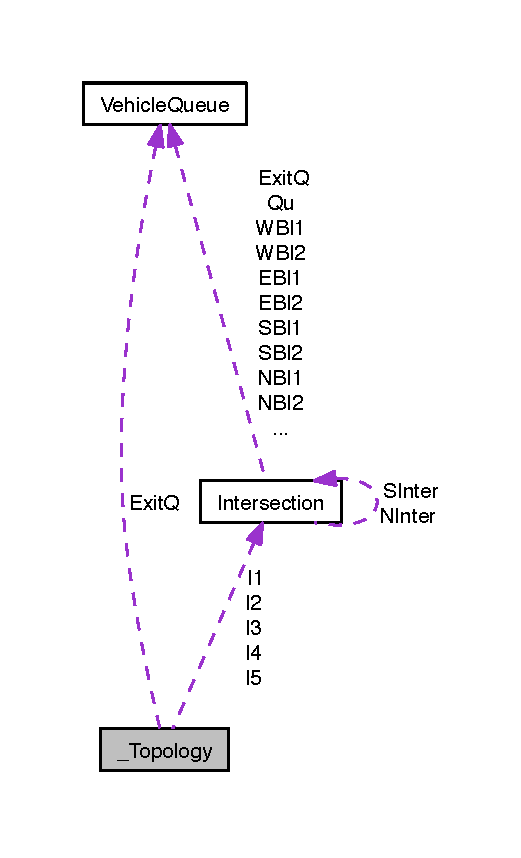
\includegraphics[width=250pt]{class___topology__coll__graph}
\end{center}
\end{figure}
\subsection*{Public Member Functions}
\begin{DoxyCompactItemize}
\item 
\hyperlink{class___topology_abe643100e153984647c440cd9ffdb50e}{\-\_\-\-Topology} ()
\end{DoxyCompactItemize}
\subsection*{Public Attributes}
\begin{DoxyCompactItemize}
\item 
\hyperlink{class_intersection}{Intersection} $\ast$ \hyperlink{class___topology_a22e676a8a8519d5e81264facc142cd4c}{I1}
\item 
\hyperlink{class_intersection}{Intersection} $\ast$ \hyperlink{class___topology_add9dde7506b1951f72fc82737a448f3e}{I2}
\item 
\hyperlink{class_intersection}{Intersection} $\ast$ \hyperlink{class___topology_a5853e98887c0354e46d72c66e434d835}{I3}
\item 
\hyperlink{class_intersection}{Intersection} $\ast$ \hyperlink{class___topology_a6ed4a6f988c5879829337e3c819acf61}{I4}
\item 
\hyperlink{class_intersection}{Intersection} $\ast$ \hyperlink{class___topology_a863a6dbc380236cc23cf4df6a9e24136}{I5}
\item 
\hypertarget{class___topology_aa6a0f1d90201b20bc625a4654908694d}{\hyperlink{class_intersection}{Intersection} $\ast$ {\bfseries In} \mbox{[}5\mbox{]}}\label{class___topology_aa6a0f1d90201b20bc625a4654908694d}

\item 
\hyperlink{class_vehicle_queue}{Vehicle\-Queue} $\ast$ \hyperlink{class___topology_a6f52e458294112feaf5ef76ab457b540}{Exit\-Q}
\end{DoxyCompactItemize}


\subsection{Constructor \& Destructor Documentation}
\hypertarget{class___topology_abe643100e153984647c440cd9ffdb50e}{\index{\-\_\-\-Topology@{\-\_\-\-Topology}!\-\_\-\-Topology@{\-\_\-\-Topology}}
\index{\-\_\-\-Topology@{\-\_\-\-Topology}!_Topology@{\-\_\-\-Topology}}
\subsubsection[{\-\_\-\-Topology}]{\setlength{\rightskip}{0pt plus 5cm}\-\_\-\-Topology\-::\-\_\-\-Topology (
\begin{DoxyParamCaption}
{}
\end{DoxyParamCaption}
)\hspace{0.3cm}{\ttfamily [inline]}}}\label{class___topology_abe643100e153984647c440cd9ffdb50e}
Default constructor Initializes the topology with intersections and 

\subsection{Member Data Documentation}
\hypertarget{class___topology_a6f52e458294112feaf5ef76ab457b540}{\index{\-\_\-\-Topology@{\-\_\-\-Topology}!Exit\-Q@{Exit\-Q}}
\index{Exit\-Q@{Exit\-Q}!_Topology@{\-\_\-\-Topology}}
\subsubsection[{Exit\-Q}]{\setlength{\rightskip}{0pt plus 5cm}{\bf Vehicle\-Queue}$\ast$ \-\_\-\-Topology\-::\-Exit\-Q}}\label{class___topology_a6f52e458294112feaf5ef76ab457b540}
Holds a vehicles queue for post processing \hypertarget{class___topology_a22e676a8a8519d5e81264facc142cd4c}{\index{\-\_\-\-Topology@{\-\_\-\-Topology}!I1@{I1}}
\index{I1@{I1}!_Topology@{\-\_\-\-Topology}}
\subsubsection[{I1}]{\setlength{\rightskip}{0pt plus 5cm}{\bf Intersection}$\ast$ \-\_\-\-Topology\-::\-I1}}\label{class___topology_a22e676a8a8519d5e81264facc142cd4c}
10th street \hypertarget{class___topology_add9dde7506b1951f72fc82737a448f3e}{\index{\-\_\-\-Topology@{\-\_\-\-Topology}!I2@{I2}}
\index{I2@{I2}!_Topology@{\-\_\-\-Topology}}
\subsubsection[{I2}]{\setlength{\rightskip}{0pt plus 5cm}{\bf Intersection}$\ast$ \-\_\-\-Topology\-::\-I2}}\label{class___topology_add9dde7506b1951f72fc82737a448f3e}
11th street \hypertarget{class___topology_a5853e98887c0354e46d72c66e434d835}{\index{\-\_\-\-Topology@{\-\_\-\-Topology}!I3@{I3}}
\index{I3@{I3}!_Topology@{\-\_\-\-Topology}}
\subsubsection[{I3}]{\setlength{\rightskip}{0pt plus 5cm}{\bf Intersection}$\ast$ \-\_\-\-Topology\-::\-I3}}\label{class___topology_a5853e98887c0354e46d72c66e434d835}
12th street \hypertarget{class___topology_a6ed4a6f988c5879829337e3c819acf61}{\index{\-\_\-\-Topology@{\-\_\-\-Topology}!I4@{I4}}
\index{I4@{I4}!_Topology@{\-\_\-\-Topology}}
\subsubsection[{I4}]{\setlength{\rightskip}{0pt plus 5cm}{\bf Intersection}$\ast$ \-\_\-\-Topology\-::\-I4}}\label{class___topology_a6ed4a6f988c5879829337e3c819acf61}
13th street \hypertarget{class___topology_a863a6dbc380236cc23cf4df6a9e24136}{\index{\-\_\-\-Topology@{\-\_\-\-Topology}!I5@{I5}}
\index{I5@{I5}!_Topology@{\-\_\-\-Topology}}
\subsubsection[{I5}]{\setlength{\rightskip}{0pt plus 5cm}{\bf Intersection}$\ast$ \-\_\-\-Topology\-::\-I5}}\label{class___topology_a863a6dbc380236cc23cf4df6a9e24136}
14th street 

The documentation for this class was generated from the following file\-:\begin{DoxyCompactItemize}
\item 
\hyperlink{_topology_8h}{Topology.\-h}\end{DoxyCompactItemize}

\hypertarget{classcalender__queue}{\section{calender\-\_\-queue Class Reference}
\label{classcalender__queue}\index{calender\-\_\-queue@{calender\-\_\-queue}}
}


{\ttfamily \#include $<$calender\-\_\-queue.\-h$>$}

\subsection*{Public Member Functions}
\begin{DoxyCompactItemize}
\item 
void \hyperlink{classcalender__queue_a9908e97c05434b58fca91d5327cf479b}{insert} (\hyperlink{class_event_base}{Event\-Base} $\ast$E1)
\item 
void \hyperlink{classcalender__queue_ad751210f4fe9885234857ca428799c18}{dequeue} (\hyperlink{class_event_base}{Event\-Base} $\ast$E1)
\item 
\hyperlink{class_event_base}{Event\-Base} $\ast$ \hyperlink{classcalender__queue_adce9f39aeb6b2912579ffc3aad67bd7a}{Pop\-Next} ()
\item 
\hyperlink{class_event_base}{Event\-Base} $\ast$ \hyperlink{classcalender__queue_ad23634e4153b9a76fee485f1c62e4c1a}{next\-\_\-event} (int bucket\-\_\-num)
\item 
void \hyperlink{classcalender__queue_a5643aa39133a7c8d62b465752c62ad88}{remove\-\_\-event} (int bucket\-\_\-num, \hyperlink{class_event_base}{Event\-Base} $\ast$E1)
\item 
int \hyperlink{classcalender__queue_a8d42460de7de2396f588c8f9a5aa099f}{is\-Empty} ()
\item 
int \hyperlink{classcalender__queue_a78818b6767d5f432dd4b4e629ca72435}{get\-\_\-bucket\-\_\-count} ()
\item 
\hyperlink{classcalender__queue_ae60c0a818d3de5b7e2e3e8f5e9919923}{calender\-\_\-queue} ()
\item 
int \hyperlink{classcalender__queue_ac6b4b6d42278a5c88de4550d4b7f4017}{get\-Qsize} ()
\item 
int \hyperlink{classcalender__queue_a3985b2b2d55245ec4b70e79e1588c608}{gettimeframe} ()
\item 
void \hyperlink{classcalender__queue_a3b911c0f17d0cac2ff6c2a261d123a78}{check659bucket} ()
\item 
void \hyperlink{classcalender__queue_a533aa5760d1e91277a071771c6f1ffb7}{init} (int num, double wid, double earliest)
\item 
void \hyperlink{classcalender__queue_a83feb3627a7f8b83e89227fccc4545d5}{resize} ()
\item 
\hypertarget{classcalender__queue_afabc6b9f3cade5ba8aca2856e65a1dd8}{void {\bfseries insert} (\hyperlink{classnode}{node} $\ast$E1)}\label{classcalender__queue_afabc6b9f3cade5ba8aca2856e65a1dd8}

\item 
void \hyperlink{classcalender__queue_a7c07ffcbca12cfd91018963c70c1542a}{dequeue} (\hyperlink{classnode}{node} $\ast$E1)
\item 
\hyperlink{classnode}{node} $\ast$ \hyperlink{classcalender__queue_adbc1d16f019e929d53e8448e98fa92b9}{Pop\-Next} ()
\item 
\hyperlink{classnode}{node} $\ast$ \hyperlink{classcalender__queue_aa75ebefb2a4219895c3b44219077c870}{next\-\_\-event} (int bucket\-\_\-num)
\item 
void \hyperlink{classcalender__queue_ac5780ed685a1c4725b53857cc525c7e7}{remove\-\_\-event} (int bucket\-\_\-num, \hyperlink{classnode}{node} $\ast$E1)
\item 
int \hyperlink{classcalender__queue_a8d42460de7de2396f588c8f9a5aa099f}{is\-Empty} ()
\item 
int \hyperlink{classcalender__queue_a78818b6767d5f432dd4b4e629ca72435}{get\-\_\-bucket\-\_\-count} ()
\item 
\hyperlink{classcalender__queue_ace3cfae6b7e3a8bcf3a5a84b270ef0f8}{calender\-\_\-queue} (int bk, double int\-\_\-width, double bk\-\_\-sz)
\item 
int \hyperlink{classcalender__queue_ac6b4b6d42278a5c88de4550d4b7f4017}{get\-Qsize} ()
\item 
int \hyperlink{classcalender__queue_a3985b2b2d55245ec4b70e79e1588c608}{gettimeframe} ()
\item 
void \hyperlink{classcalender__queue_a3b911c0f17d0cac2ff6c2a261d123a78}{check659bucket} ()
\end{DoxyCompactItemize}


\subsection{Detailed Description}
Calender Queue is priority queue, Ref\-: Calendar queues\-: a fast 0(1) priority queue implementation for the simulation event set problem 

\subsection{Constructor \& Destructor Documentation}
\hypertarget{classcalender__queue_ae60c0a818d3de5b7e2e3e8f5e9919923}{\index{calender\-\_\-queue@{calender\-\_\-queue}!calender\-\_\-queue@{calender\-\_\-queue}}
\index{calender\-\_\-queue@{calender\-\_\-queue}!calender_queue@{calender\-\_\-queue}}
\subsubsection[{calender\-\_\-queue}]{\setlength{\rightskip}{0pt plus 5cm}calender\-\_\-queue\-::calender\-\_\-queue (
\begin{DoxyParamCaption}
{}
\end{DoxyParamCaption}
)}}\label{classcalender__queue_ae60c0a818d3de5b7e2e3e8f5e9919923}
Default constructor \hypertarget{classcalender__queue_ace3cfae6b7e3a8bcf3a5a84b270ef0f8}{\index{calender\-\_\-queue@{calender\-\_\-queue}!calender\-\_\-queue@{calender\-\_\-queue}}
\index{calender\-\_\-queue@{calender\-\_\-queue}!calender_queue@{calender\-\_\-queue}}
\subsubsection[{calender\-\_\-queue}]{\setlength{\rightskip}{0pt plus 5cm}calender\-\_\-queue\-::calender\-\_\-queue (
\begin{DoxyParamCaption}
\item[{int}]{bk, }
\item[{double}]{int\-\_\-width, }
\item[{double}]{bk\-\_\-sz}
\end{DoxyParamCaption}
)}}\label{classcalender__queue_ace3cfae6b7e3a8bcf3a5a84b270ef0f8}
Default constructor constructs an calender queue with buck\-\_\-count number of buckets 

\subsection{Member Function Documentation}
\hypertarget{classcalender__queue_a3b911c0f17d0cac2ff6c2a261d123a78}{\index{calender\-\_\-queue@{calender\-\_\-queue}!check659bucket@{check659bucket}}
\index{check659bucket@{check659bucket}!calender_queue@{calender\-\_\-queue}}
\subsubsection[{check659bucket}]{\setlength{\rightskip}{0pt plus 5cm}void calender\-\_\-queue\-::check659bucket (
\begin{DoxyParamCaption}
{}
\end{DoxyParamCaption}
)}}\label{classcalender__queue_a3b911c0f17d0cac2ff6c2a261d123a78}
is there debuggin purpose \hypertarget{classcalender__queue_a3b911c0f17d0cac2ff6c2a261d123a78}{\index{calender\-\_\-queue@{calender\-\_\-queue}!check659bucket@{check659bucket}}
\index{check659bucket@{check659bucket}!calender_queue@{calender\-\_\-queue}}
\subsubsection[{check659bucket}]{\setlength{\rightskip}{0pt plus 5cm}void calender\-\_\-queue\-::check659bucket (
\begin{DoxyParamCaption}
{}
\end{DoxyParamCaption}
)}}\label{classcalender__queue_a3b911c0f17d0cac2ff6c2a261d123a78}
is there debuggin purpose \hypertarget{classcalender__queue_ad751210f4fe9885234857ca428799c18}{\index{calender\-\_\-queue@{calender\-\_\-queue}!dequeue@{dequeue}}
\index{dequeue@{dequeue}!calender_queue@{calender\-\_\-queue}}
\subsubsection[{dequeue}]{\setlength{\rightskip}{0pt plus 5cm}void calender\-\_\-queue\-::dequeue (
\begin{DoxyParamCaption}
\item[{{\bf Event\-Base} $\ast$}]{E1}
\end{DoxyParamCaption}
)}}\label{classcalender__queue_ad751210f4fe9885234857ca428799c18}
Removes an event E1 from the list (Hence it won't be scheduled) 
\begin{DoxyParams}{Parameters}
{\em E1} & \-: event pointer to removed from the list \\
\hline
\end{DoxyParams}
\hypertarget{classcalender__queue_a7c07ffcbca12cfd91018963c70c1542a}{\index{calender\-\_\-queue@{calender\-\_\-queue}!dequeue@{dequeue}}
\index{dequeue@{dequeue}!calender_queue@{calender\-\_\-queue}}
\subsubsection[{dequeue}]{\setlength{\rightskip}{0pt plus 5cm}void calender\-\_\-queue\-::dequeue (
\begin{DoxyParamCaption}
\item[{{\bf node} $\ast$}]{E1}
\end{DoxyParamCaption}
)}}\label{classcalender__queue_a7c07ffcbca12cfd91018963c70c1542a}
Removes an event E1 from the list (Hence it won't be scheduled) 
\begin{DoxyParams}{Parameters}
{\em E1} & \-: event pointer to removed from the list \\
\hline
\end{DoxyParams}


Here is the call graph for this function\-:
\nopagebreak
\begin{figure}[H]
\begin{center}
\leavevmode
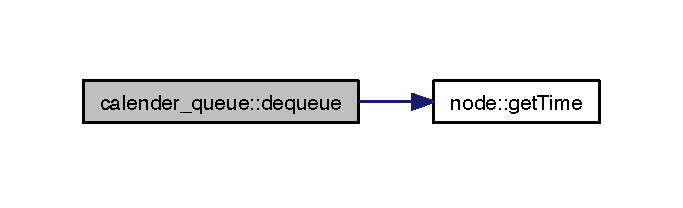
\includegraphics[width=328pt]{classcalender__queue_a7c07ffcbca12cfd91018963c70c1542a_cgraph}
\end{center}
\end{figure}


\hypertarget{classcalender__queue_a78818b6767d5f432dd4b4e629ca72435}{\index{calender\-\_\-queue@{calender\-\_\-queue}!get\-\_\-bucket\-\_\-count@{get\-\_\-bucket\-\_\-count}}
\index{get\-\_\-bucket\-\_\-count@{get\-\_\-bucket\-\_\-count}!calender_queue@{calender\-\_\-queue}}
\subsubsection[{get\-\_\-bucket\-\_\-count}]{\setlength{\rightskip}{0pt plus 5cm}int calender\-\_\-queue\-::get\-\_\-bucket\-\_\-count (
\begin{DoxyParamCaption}
{}
\end{DoxyParamCaption}
)}}\label{classcalender__queue_a78818b6767d5f432dd4b4e629ca72435}
Get number of buckets in the calender queue \hypertarget{classcalender__queue_a78818b6767d5f432dd4b4e629ca72435}{\index{calender\-\_\-queue@{calender\-\_\-queue}!get\-\_\-bucket\-\_\-count@{get\-\_\-bucket\-\_\-count}}
\index{get\-\_\-bucket\-\_\-count@{get\-\_\-bucket\-\_\-count}!calender_queue@{calender\-\_\-queue}}
\subsubsection[{get\-\_\-bucket\-\_\-count}]{\setlength{\rightskip}{0pt plus 5cm}int calender\-\_\-queue\-::get\-\_\-bucket\-\_\-count (
\begin{DoxyParamCaption}
{}
\end{DoxyParamCaption}
)}}\label{classcalender__queue_a78818b6767d5f432dd4b4e629ca72435}
Get number of buckets in the calender queue \hypertarget{classcalender__queue_ac6b4b6d42278a5c88de4550d4b7f4017}{\index{calender\-\_\-queue@{calender\-\_\-queue}!get\-Qsize@{get\-Qsize}}
\index{get\-Qsize@{get\-Qsize}!calender_queue@{calender\-\_\-queue}}
\subsubsection[{get\-Qsize}]{\setlength{\rightskip}{0pt plus 5cm}int calender\-\_\-queue\-::get\-Qsize (
\begin{DoxyParamCaption}
{}
\end{DoxyParamCaption}
)}}\label{classcalender__queue_ac6b4b6d42278a5c88de4550d4b7f4017}
Returns number of element in the Q \hypertarget{classcalender__queue_ac6b4b6d42278a5c88de4550d4b7f4017}{\index{calender\-\_\-queue@{calender\-\_\-queue}!get\-Qsize@{get\-Qsize}}
\index{get\-Qsize@{get\-Qsize}!calender_queue@{calender\-\_\-queue}}
\subsubsection[{get\-Qsize}]{\setlength{\rightskip}{0pt plus 5cm}int calender\-\_\-queue\-::get\-Qsize (
\begin{DoxyParamCaption}
{}
\end{DoxyParamCaption}
)}}\label{classcalender__queue_ac6b4b6d42278a5c88de4550d4b7f4017}
Returns number of element in the Q \hypertarget{classcalender__queue_a3985b2b2d55245ec4b70e79e1588c608}{\index{calender\-\_\-queue@{calender\-\_\-queue}!gettimeframe@{gettimeframe}}
\index{gettimeframe@{gettimeframe}!calender_queue@{calender\-\_\-queue}}
\subsubsection[{gettimeframe}]{\setlength{\rightskip}{0pt plus 5cm}int calender\-\_\-queue\-::gettimeframe (
\begin{DoxyParamCaption}
{}
\end{DoxyParamCaption}
)}}\label{classcalender__queue_a3985b2b2d55245ec4b70e79e1588c608}
Returns the time frame from which last event was popped \hypertarget{classcalender__queue_a3985b2b2d55245ec4b70e79e1588c608}{\index{calender\-\_\-queue@{calender\-\_\-queue}!gettimeframe@{gettimeframe}}
\index{gettimeframe@{gettimeframe}!calender_queue@{calender\-\_\-queue}}
\subsubsection[{gettimeframe}]{\setlength{\rightskip}{0pt plus 5cm}int calender\-\_\-queue\-::gettimeframe (
\begin{DoxyParamCaption}
{}
\end{DoxyParamCaption}
)}}\label{classcalender__queue_a3985b2b2d55245ec4b70e79e1588c608}
Returns the time frame from which last event was popped \hypertarget{classcalender__queue_a533aa5760d1e91277a071771c6f1ffb7}{\index{calender\-\_\-queue@{calender\-\_\-queue}!init@{init}}
\index{init@{init}!calender_queue@{calender\-\_\-queue}}
\subsubsection[{init}]{\setlength{\rightskip}{0pt plus 5cm}void calender\-\_\-queue\-::init (
\begin{DoxyParamCaption}
\item[{int}]{num, }
\item[{double}]{wid, }
\item[{double}]{earliest}
\end{DoxyParamCaption}
)}}\label{classcalender__queue_a533aa5760d1e91277a071771c6f1ffb7}
Initilizes the queue with num buckets \hypertarget{classcalender__queue_a9908e97c05434b58fca91d5327cf479b}{\index{calender\-\_\-queue@{calender\-\_\-queue}!insert@{insert}}
\index{insert@{insert}!calender_queue@{calender\-\_\-queue}}
\subsubsection[{insert}]{\setlength{\rightskip}{0pt plus 5cm}void calender\-\_\-queue\-::insert (
\begin{DoxyParamCaption}
\item[{{\bf Event\-Base} $\ast$}]{E1}
\end{DoxyParamCaption}
)}}\label{classcalender__queue_a9908e97c05434b58fca91d5327cf479b}
Inserts an event into the priority list 
\begin{DoxyParams}{Parameters}
{\em E1} & is the even to be inserted into the list \\
\hline
\end{DoxyParams}
\hypertarget{classcalender__queue_a8d42460de7de2396f588c8f9a5aa099f}{\index{calender\-\_\-queue@{calender\-\_\-queue}!is\-Empty@{is\-Empty}}
\index{is\-Empty@{is\-Empty}!calender_queue@{calender\-\_\-queue}}
\subsubsection[{is\-Empty}]{\setlength{\rightskip}{0pt plus 5cm}int calender\-\_\-queue\-::is\-Empty (
\begin{DoxyParamCaption}
{}
\end{DoxyParamCaption}
)}}\label{classcalender__queue_a8d42460de7de2396f588c8f9a5aa099f}
Checks if there are anymore events left in the list \hypertarget{classcalender__queue_a8d42460de7de2396f588c8f9a5aa099f}{\index{calender\-\_\-queue@{calender\-\_\-queue}!is\-Empty@{is\-Empty}}
\index{is\-Empty@{is\-Empty}!calender_queue@{calender\-\_\-queue}}
\subsubsection[{is\-Empty}]{\setlength{\rightskip}{0pt plus 5cm}int calender\-\_\-queue\-::is\-Empty (
\begin{DoxyParamCaption}
{}
\end{DoxyParamCaption}
)}}\label{classcalender__queue_a8d42460de7de2396f588c8f9a5aa099f}
Checks if there are anymore events left in the list \hypertarget{classcalender__queue_ad23634e4153b9a76fee485f1c62e4c1a}{\index{calender\-\_\-queue@{calender\-\_\-queue}!next\-\_\-event@{next\-\_\-event}}
\index{next\-\_\-event@{next\-\_\-event}!calender_queue@{calender\-\_\-queue}}
\subsubsection[{next\-\_\-event}]{\setlength{\rightskip}{0pt plus 5cm}{\bf node} $\ast$ calender\-\_\-queue\-::next\-\_\-event (
\begin{DoxyParamCaption}
\item[{int}]{bucket\-\_\-num}
\end{DoxyParamCaption}
)}}\label{classcalender__queue_ad23634e4153b9a76fee485f1c62e4c1a}
Returns event with minimum time from bucket-\/num 
\begin{DoxyParams}{Parameters}
{\em bucket\-\_\-num} & is the number of bucket from which you want to get the min time stamp event \\
\hline
\end{DoxyParams}
\hypertarget{classcalender__queue_aa75ebefb2a4219895c3b44219077c870}{\index{calender\-\_\-queue@{calender\-\_\-queue}!next\-\_\-event@{next\-\_\-event}}
\index{next\-\_\-event@{next\-\_\-event}!calender_queue@{calender\-\_\-queue}}
\subsubsection[{next\-\_\-event}]{\setlength{\rightskip}{0pt plus 5cm}{\bf node}$\ast$ calender\-\_\-queue\-::next\-\_\-event (
\begin{DoxyParamCaption}
\item[{int}]{bucket\-\_\-num}
\end{DoxyParamCaption}
)}}\label{classcalender__queue_aa75ebefb2a4219895c3b44219077c870}
Returns event with minimum time from bucket-\/num 
\begin{DoxyParams}{Parameters}
{\em bucket\-\_\-num} & is the number of bucket from which you want to get the min time stamp event \\
\hline
\end{DoxyParams}
\hypertarget{classcalender__queue_adce9f39aeb6b2912579ffc3aad67bd7a}{\index{calender\-\_\-queue@{calender\-\_\-queue}!Pop\-Next@{Pop\-Next}}
\index{Pop\-Next@{Pop\-Next}!calender_queue@{calender\-\_\-queue}}
\subsubsection[{Pop\-Next}]{\setlength{\rightskip}{0pt plus 5cm}{\bf node} $\ast$ calender\-\_\-queue\-::\-Pop\-Next (
\begin{DoxyParamCaption}
{}
\end{DoxyParamCaption}
)}}\label{classcalender__queue_adce9f39aeb6b2912579ffc3aad67bd7a}
Pops Next event(event with minimum time stamp) in the list (and removes it as well) \begin{DoxyReturn}{Returns}
Event pointer with minimum time stamp 
\end{DoxyReturn}


Here is the call graph for this function\-:
\nopagebreak
\begin{figure}[H]
\begin{center}
\leavevmode
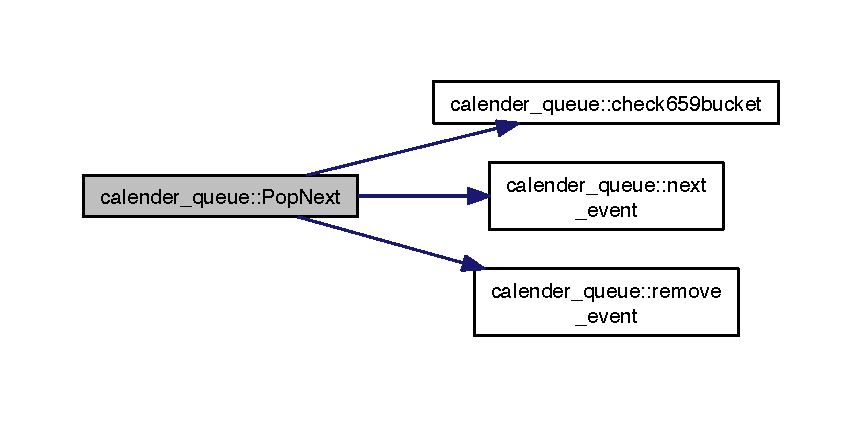
\includegraphics[width=350pt]{classcalender__queue_adce9f39aeb6b2912579ffc3aad67bd7a_cgraph}
\end{center}
\end{figure}


\hypertarget{classcalender__queue_adbc1d16f019e929d53e8448e98fa92b9}{\index{calender\-\_\-queue@{calender\-\_\-queue}!Pop\-Next@{Pop\-Next}}
\index{Pop\-Next@{Pop\-Next}!calender_queue@{calender\-\_\-queue}}
\subsubsection[{Pop\-Next}]{\setlength{\rightskip}{0pt plus 5cm}{\bf node}$\ast$ calender\-\_\-queue\-::\-Pop\-Next (
\begin{DoxyParamCaption}
{}
\end{DoxyParamCaption}
)}}\label{classcalender__queue_adbc1d16f019e929d53e8448e98fa92b9}
Pops Next event(event with minimum time stamp) in the list (and removes it as well) \begin{DoxyReturn}{Returns}
Event pointer with minimum time stamp 
\end{DoxyReturn}
\hypertarget{classcalender__queue_a5643aa39133a7c8d62b465752c62ad88}{\index{calender\-\_\-queue@{calender\-\_\-queue}!remove\-\_\-event@{remove\-\_\-event}}
\index{remove\-\_\-event@{remove\-\_\-event}!calender_queue@{calender\-\_\-queue}}
\subsubsection[{remove\-\_\-event}]{\setlength{\rightskip}{0pt plus 5cm}void calender\-\_\-queue\-::remove\-\_\-event (
\begin{DoxyParamCaption}
\item[{int}]{bucket\-\_\-num, }
\item[{{\bf Event\-Base} $\ast$}]{E1}
\end{DoxyParamCaption}
)}}\label{classcalender__queue_a5643aa39133a7c8d62b465752c62ad88}
Removes event E1 from bucket\-\_\-num$^\wedge$th bucket 
\begin{DoxyParams}{Parameters}
{\em B\-Ucket\-\_\-num} & is the id of bucket from which event is to be removed \\
\hline
{\em E1} & is pointer to event to be removed \\
\hline
\end{DoxyParams}
\hypertarget{classcalender__queue_ac5780ed685a1c4725b53857cc525c7e7}{\index{calender\-\_\-queue@{calender\-\_\-queue}!remove\-\_\-event@{remove\-\_\-event}}
\index{remove\-\_\-event@{remove\-\_\-event}!calender_queue@{calender\-\_\-queue}}
\subsubsection[{remove\-\_\-event}]{\setlength{\rightskip}{0pt plus 5cm}void calender\-\_\-queue\-::remove\-\_\-event (
\begin{DoxyParamCaption}
\item[{int}]{bucket\-\_\-num, }
\item[{{\bf node} $\ast$}]{E1}
\end{DoxyParamCaption}
)}}\label{classcalender__queue_ac5780ed685a1c4725b53857cc525c7e7}
Removes event E1 from bucket\-\_\-num$^\wedge$th bucket 
\begin{DoxyParams}{Parameters}
{\em B\-Ucket\-\_\-num} & is the id of bucket from which event is to be removed \\
\hline
{\em E1} & is pointer to event to be removed \\
\hline
\end{DoxyParams}
\hypertarget{classcalender__queue_a83feb3627a7f8b83e89227fccc4545d5}{\index{calender\-\_\-queue@{calender\-\_\-queue}!resize@{resize}}
\index{resize@{resize}!calender_queue@{calender\-\_\-queue}}
\subsubsection[{resize}]{\setlength{\rightskip}{0pt plus 5cm}void calender\-\_\-queue\-::resize (
\begin{DoxyParamCaption}
{}
\end{DoxyParamCaption}
)}}\label{classcalender__queue_a83feb3627a7f8b83e89227fccc4545d5}
Inserts an event into the priority list 
\begin{DoxyParams}{Parameters}
{\em E1} & is the even to be inserted into the list Resizes the calender queue based on \\
\hline
\end{DoxyParams}


The documentation for this class was generated from the following files\-:\begin{DoxyCompactItemize}
\item 
\hyperlink{calender__queue_8h}{calender\-\_\-queue.\-h}\item 
testing/calender\-\_\-queue\-\_\-testing.\-h\item 
calender\-\_\-queue.\-cc\item 
testing/calender\-\_\-queue\-\_\-testing.\-cc\end{DoxyCompactItemize}

\hypertarget{class_event0}{\section{Event0$<$ T, O\-B\-J $>$ Class Template Reference}
\label{class_event0}\index{Event0$<$ T, O\-B\-J $>$@{Event0$<$ T, O\-B\-J $>$}}
}


Inheritance diagram for Event0$<$ T, O\-B\-J $>$\-:\nopagebreak
\begin{figure}[H]
\begin{center}
\leavevmode
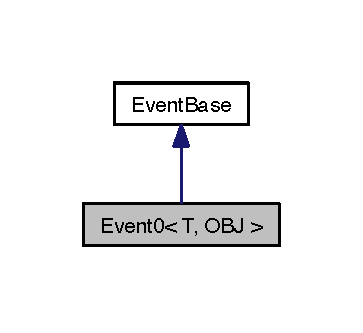
\includegraphics[width=174pt]{class_event0__inherit__graph}
\end{center}
\end{figure}


Collaboration diagram for Event0$<$ T, O\-B\-J $>$\-:\nopagebreak
\begin{figure}[H]
\begin{center}
\leavevmode
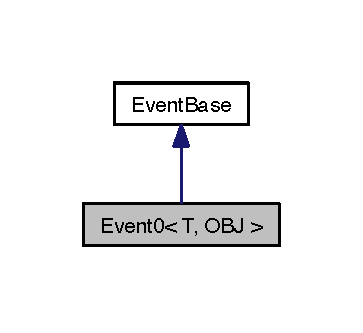
\includegraphics[width=174pt]{class_event0__coll__graph}
\end{center}
\end{figure}
\subsection*{Public Member Functions}
\begin{DoxyCompactItemize}
\item 
\hypertarget{class_event0_a71a74bee8ececd124b7928bc31a662cf}{{\bfseries Event0} (double t, void(T\-::$\ast$f)(), O\-B\-J $\ast$obj0)}\label{class_event0_a71a74bee8ececd124b7928bc31a662cf}

\item 
\hypertarget{class_event0_a77176d1040ed4cc48fa750c4854212b9}{void {\bfseries Call\-Handler} ()}\label{class_event0_a77176d1040ed4cc48fa750c4854212b9}

\end{DoxyCompactItemize}
\subsection*{Public Attributes}
\begin{DoxyCompactItemize}
\item 
\hypertarget{class_event0_a9f5c4b04f0f887ef7a2df146e10e9403}{void(T\-::$\ast$ {\bfseries handler} )(void)}\label{class_event0_a9f5c4b04f0f887ef7a2df146e10e9403}

\item 
\hypertarget{class_event0_ab37236e93d14993e36a8913ae2dbaf31}{O\-B\-J $\ast$ {\bfseries obj}}\label{class_event0_ab37236e93d14993e36a8913ae2dbaf31}

\end{DoxyCompactItemize}


The documentation for this class was generated from the following file\-:\begin{DoxyCompactItemize}
\item 
Events.\-h\end{DoxyCompactItemize}

\hypertarget{class_event1}{\section{Event1$<$ T, O\-B\-J, U1, T1 $>$ Class Template Reference}
\label{class_event1}\index{Event1$<$ T, O\-B\-J, U1, T1 $>$@{Event1$<$ T, O\-B\-J, U1, T1 $>$}}
}


Inheritance diagram for Event1$<$ T, O\-B\-J, U1, T1 $>$\-:\nopagebreak
\begin{figure}[H]
\begin{center}
\leavevmode
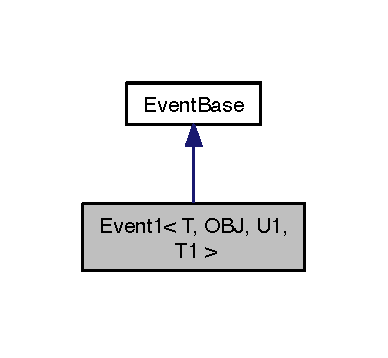
\includegraphics[width=186pt]{class_event1__inherit__graph}
\end{center}
\end{figure}


Collaboration diagram for Event1$<$ T, O\-B\-J, U1, T1 $>$\-:\nopagebreak
\begin{figure}[H]
\begin{center}
\leavevmode
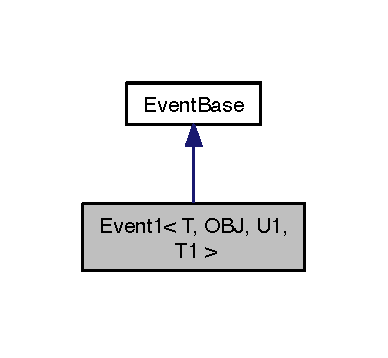
\includegraphics[width=186pt]{class_event1__coll__graph}
\end{center}
\end{figure}
\subsection*{Public Member Functions}
\begin{DoxyCompactItemize}
\item 
\hypertarget{class_event1_ae53edac1393d2f7920f936ba6c7f90ba}{{\bfseries Event1} (double t, void(T\-::$\ast$f)(U1), O\-B\-J $\ast$obj0, T1 t1\-\_\-0)}\label{class_event1_ae53edac1393d2f7920f936ba6c7f90ba}

\item 
\hypertarget{class_event1_a6d7e716e16ab6ee6672807250860cdd8}{void {\bfseries Call\-Handler} ()}\label{class_event1_a6d7e716e16ab6ee6672807250860cdd8}

\end{DoxyCompactItemize}
\subsection*{Public Attributes}
\begin{DoxyCompactItemize}
\item 
\hypertarget{class_event1_a2a02ab5cbd37a2879c3db25cf3faf80f}{void(T\-::$\ast$ {\bfseries handler} )(U1)}\label{class_event1_a2a02ab5cbd37a2879c3db25cf3faf80f}

\item 
\hypertarget{class_event1_adc793df07c00b32a012cf45b31b9d2e6}{O\-B\-J $\ast$ {\bfseries obj}}\label{class_event1_adc793df07c00b32a012cf45b31b9d2e6}

\item 
\hypertarget{class_event1_a1af2759e05940a423f3b9409feab75f9}{T1 {\bfseries t1}}\label{class_event1_a1af2759e05940a423f3b9409feab75f9}

\end{DoxyCompactItemize}


The documentation for this class was generated from the following file\-:\begin{DoxyCompactItemize}
\item 
Events.\-h\end{DoxyCompactItemize}

\hypertarget{class_event2}{\section{Event2$<$ T, O\-B\-J, U1, T1, U2, T2 $>$ Class Template Reference}
\label{class_event2}\index{Event2$<$ T, O\-B\-J, U1, T1, U2, T2 $>$@{Event2$<$ T, O\-B\-J, U1, T1, U2, T2 $>$}}
}


Inheritance diagram for Event2$<$ T, O\-B\-J, U1, T1, U2, T2 $>$\-:\nopagebreak
\begin{figure}[H]
\begin{center}
\leavevmode
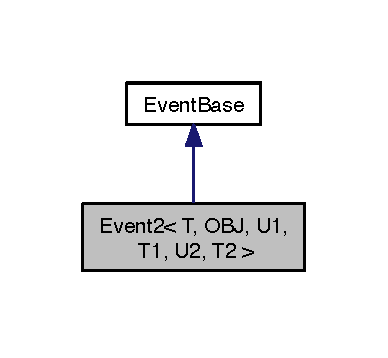
\includegraphics[width=186pt]{class_event2__inherit__graph}
\end{center}
\end{figure}


Collaboration diagram for Event2$<$ T, O\-B\-J, U1, T1, U2, T2 $>$\-:\nopagebreak
\begin{figure}[H]
\begin{center}
\leavevmode
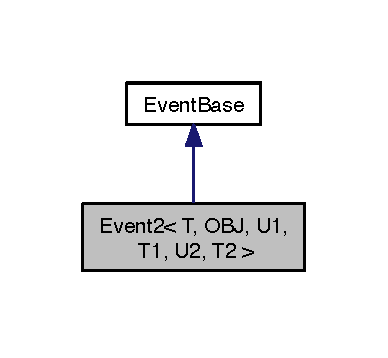
\includegraphics[width=186pt]{class_event2__coll__graph}
\end{center}
\end{figure}
\subsection*{Public Member Functions}
\begin{DoxyCompactItemize}
\item 
\hypertarget{class_event2_aba7c624909641184917f7a5603ab2ebe}{{\bfseries Event2} (double t, void(T\-::$\ast$f)(U1, U2), O\-B\-J $\ast$obj0, T1 t1\-\_\-0, T2 t2\-\_\-0)}\label{class_event2_aba7c624909641184917f7a5603ab2ebe}

\item 
\hypertarget{class_event2_a428b314837eee680fa435cad61944af3}{void {\bfseries Call\-Handler} ()}\label{class_event2_a428b314837eee680fa435cad61944af3}

\end{DoxyCompactItemize}
\subsection*{Public Attributes}
\begin{DoxyCompactItemize}
\item 
\hypertarget{class_event2_a166c37cb53b2969dac38fa79b0349768}{void(T\-::$\ast$ {\bfseries handler} )(U1, U2)}\label{class_event2_a166c37cb53b2969dac38fa79b0349768}

\item 
\hypertarget{class_event2_ae87200a757f09d76ae6aa5abd293f062}{O\-B\-J $\ast$ {\bfseries obj}}\label{class_event2_ae87200a757f09d76ae6aa5abd293f062}

\item 
\hypertarget{class_event2_ab3e9b3c8ae4bff79e765e54a4947f371}{T1 {\bfseries t1}}\label{class_event2_ab3e9b3c8ae4bff79e765e54a4947f371}

\item 
\hypertarget{class_event2_ad921b4a0baa31fa2400fd022bf3b43e9}{T2 {\bfseries t2}}\label{class_event2_ad921b4a0baa31fa2400fd022bf3b43e9}

\end{DoxyCompactItemize}


The documentation for this class was generated from the following file\-:\begin{DoxyCompactItemize}
\item 
\hyperlink{_events_8h}{Events.\-h}\end{DoxyCompactItemize}

\hypertarget{class_event3}{\section{Event3$<$ T, O\-B\-J, U1, T1, U2, T2, U3, T3 $>$ Class Template Reference}
\label{class_event3}\index{Event3$<$ T, O\-B\-J, U1, T1, U2, T2, U3, T3 $>$@{Event3$<$ T, O\-B\-J, U1, T1, U2, T2, U3, T3 $>$}}
}


Inheritance diagram for Event3$<$ T, O\-B\-J, U1, T1, U2, T2, U3, T3 $>$\-:\nopagebreak
\begin{figure}[H]
\begin{center}
\leavevmode
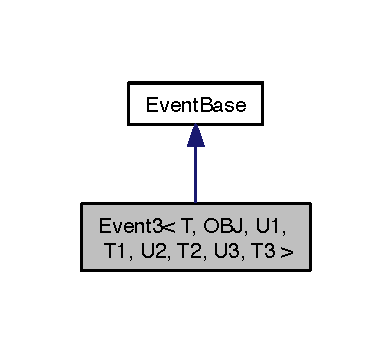
\includegraphics[width=188pt]{class_event3__inherit__graph}
\end{center}
\end{figure}


Collaboration diagram for Event3$<$ T, O\-B\-J, U1, T1, U2, T2, U3, T3 $>$\-:\nopagebreak
\begin{figure}[H]
\begin{center}
\leavevmode
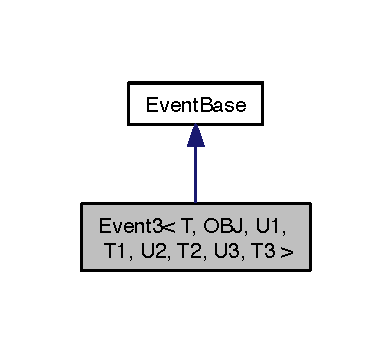
\includegraphics[width=188pt]{class_event3__coll__graph}
\end{center}
\end{figure}
\subsection*{Public Member Functions}
\begin{DoxyCompactItemize}
\item 
\hypertarget{class_event3_aab6870a823964c1843b897de6ce2057c}{{\bfseries Event3} (double t, void(T\-::$\ast$f)(U1, U2, U3), O\-B\-J $\ast$obj0, T1 t1\-\_\-0, T2 t2\-\_\-0, T3 t3\-\_\-0)}\label{class_event3_aab6870a823964c1843b897de6ce2057c}

\item 
\hypertarget{class_event3_a1b9501d43723072952055c5abd9dc9be}{void {\bfseries Call\-Handler} ()}\label{class_event3_a1b9501d43723072952055c5abd9dc9be}

\end{DoxyCompactItemize}
\subsection*{Public Attributes}
\begin{DoxyCompactItemize}
\item 
\hypertarget{class_event3_a2b4a3b7dbddc1dc7954942e7b2fe5745}{void(T\-::$\ast$ {\bfseries handler} )(U1, U2, U3)}\label{class_event3_a2b4a3b7dbddc1dc7954942e7b2fe5745}

\item 
\hypertarget{class_event3_adf320f52db00df12079299c183cb84d0}{O\-B\-J $\ast$ {\bfseries obj}}\label{class_event3_adf320f52db00df12079299c183cb84d0}

\item 
\hypertarget{class_event3_ad42449bd6cd4193bfb6557dc54c51eb8}{T1 {\bfseries t1}}\label{class_event3_ad42449bd6cd4193bfb6557dc54c51eb8}

\item 
\hypertarget{class_event3_a40afc3cdc9d75a5b3163795b78a42497}{T2 {\bfseries t2}}\label{class_event3_a40afc3cdc9d75a5b3163795b78a42497}

\item 
\hypertarget{class_event3_a7aa650837c6a02999bcad51817b144ef}{T3 {\bfseries t3}}\label{class_event3_a7aa650837c6a02999bcad51817b144ef}

\end{DoxyCompactItemize}


The documentation for this class was generated from the following file\-:\begin{DoxyCompactItemize}
\item 
\hyperlink{_events_8h}{Events.\-h}\end{DoxyCompactItemize}

\hypertarget{classevent__compare}{\section{event\-\_\-compare Class Reference}
\label{classevent__compare}\index{event\-\_\-compare@{event\-\_\-compare}}
}
\subsection*{Public Member Functions}
\begin{DoxyCompactItemize}
\item 
\hypertarget{classevent__compare_aa518df542cf3237d52108959a623fddf}{bool {\bfseries operator()} (\hyperlink{class_event_base}{Event\-Base} $\ast$const \&l, const \hyperlink{class_event_base}{Event\-Base} $\ast$const \&r) const }\label{classevent__compare_aa518df542cf3237d52108959a623fddf}

\end{DoxyCompactItemize}


The documentation for this class was generated from the following file\-:\begin{DoxyCompactItemize}
\item 
\hyperlink{_events_8h}{Events.\-h}\end{DoxyCompactItemize}

\hypertarget{class_event_base}{\section{Event\-Base Class Reference}
\label{class_event_base}\index{Event\-Base@{Event\-Base}}
}


Inheritance diagram for Event\-Base\-:\nopagebreak
\begin{figure}[H]
\begin{center}
\leavevmode
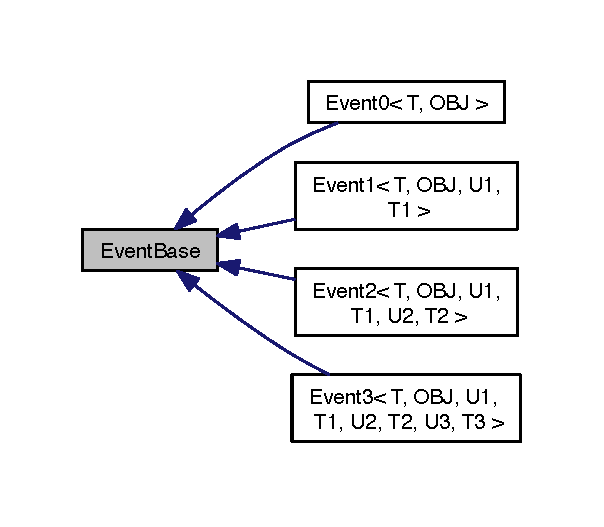
\includegraphics[width=290pt]{class_event_base__inherit__graph}
\end{center}
\end{figure}
\subsection*{Public Member Functions}
\begin{DoxyCompactItemize}
\item 
\hypertarget{class_event_base_a69050713e15086d940248753af41b50f}{{\bfseries Event\-Base} (\hyperlink{_common_defs_8h_a80b23eab88362163e2edd1a8b8238ef1}{Time\-\_\-t} t)}\label{class_event_base_a69050713e15086d940248753af41b50f}

\item 
\hypertarget{class_event_base_a121ca64dec88c8d9589c064b0060d037}{virtual void {\bfseries Call\-Handler} ()=0}\label{class_event_base_a121ca64dec88c8d9589c064b0060d037}

\item 
\hypertarget{class_event_base_abf175c0914e2ac5f5d5454868c676959}{\hyperlink{_common_defs_8h_a80b23eab88362163e2edd1a8b8238ef1}{Time\-\_\-t} {\bfseries get\-Time} ()}\label{class_event_base_abf175c0914e2ac5f5d5454868c676959}

\end{DoxyCompactItemize}
\subsection*{Public Attributes}
\begin{DoxyCompactItemize}
\item 
\hypertarget{class_event_base_aa12d9278a8b9577b1a19099963a75702}{\hyperlink{_common_defs_8h_a80b23eab88362163e2edd1a8b8238ef1}{Time\-\_\-t} {\bfseries time}}\label{class_event_base_aa12d9278a8b9577b1a19099963a75702}

\end{DoxyCompactItemize}


The documentation for this class was generated from the following file\-:\begin{DoxyCompactItemize}
\item 
\hyperlink{_events_8h}{Events.\-h}\end{DoxyCompactItemize}

\hypertarget{structevent_dsc}{\section{event\-Dsc Struct Reference}
\label{structevent_dsc}\index{event\-Dsc@{event\-Dsc}}
}
\subsection*{Public Attributes}
\begin{DoxyCompactItemize}
\item 
\hypertarget{structevent_dsc_a7de878b8aa351b4e60a4dedeffc72ac8}{int {\bfseries type}}\label{structevent_dsc_a7de878b8aa351b4e60a4dedeffc72ac8}

\item 
\hypertarget{structevent_dsc_a2310f1f76d4c059159d28ca2b5fe6b4d}{int {\bfseries Inter\-I\-D}}\label{structevent_dsc_a2310f1f76d4c059159d28ca2b5fe6b4d}

\item 
\hypertarget{structevent_dsc_a382b2e111683f5fb926daf3c1dddd819}{int {\bfseries Q\-Dir}}\label{structevent_dsc_a382b2e111683f5fb926daf3c1dddd819}

\item 
\hypertarget{structevent_dsc_aa898dbf105b9237a5a9ee9af19ca8414}{int {\bfseries Q\-Lane}}\label{structevent_dsc_aa898dbf105b9237a5a9ee9af19ca8414}

\item 
\hypertarget{structevent_dsc_a62797134a94e01b72874af3d4974589e}{int {\bfseries Q\-Size}}\label{structevent_dsc_a62797134a94e01b72874af3d4974589e}

\item 
\hypertarget{structevent_dsc_a88587beaba3370682ffca5a45c6ab87b}{double {\bfseries timetag}}\label{structevent_dsc_a88587beaba3370682ffca5a45c6ab87b}

\end{DoxyCompactItemize}


The documentation for this struct was generated from the following file\-:\begin{DoxyCompactItemize}
\item 
testing/test1.\-h\end{DoxyCompactItemize}

\hypertarget{class_intersection}{\section{Intersection Class Reference}
\label{class_intersection}\index{Intersection@{Intersection}}
}


Inheritance diagram for Intersection\-:\nopagebreak
\begin{figure}[H]
\begin{center}
\leavevmode
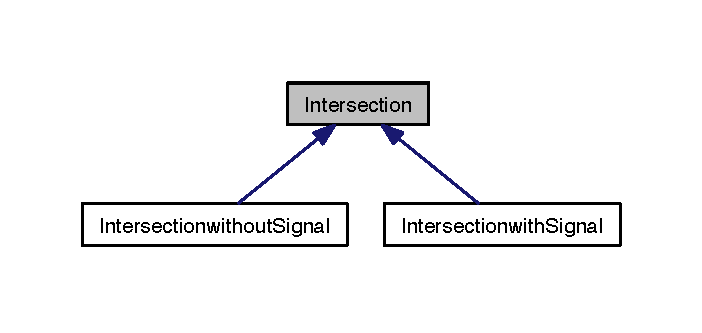
\includegraphics[width=337pt]{class_intersection__inherit__graph}
\end{center}
\end{figure}


Collaboration diagram for Intersection\-:\nopagebreak
\begin{figure}[H]
\begin{center}
\leavevmode
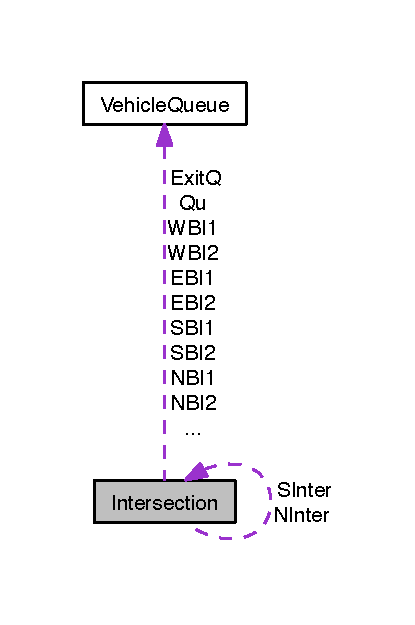
\includegraphics[width=199pt]{class_intersection__coll__graph}
\end{center}
\end{figure}
\subsection*{Public Member Functions}
\begin{DoxyCompactItemize}
\item 
\hyperlink{class_intersection_a67497e3efe2793b23909052eeb82c4f3}{Intersection} ()
\item 
\hyperlink{class_intersection_ac4c8289c83f612558e3ebbb0af571235}{Intersection} (int num)
\item 
\hyperlink{class_intersection_a064951a970ed8dd11081b2903ab62122}{$\sim$\-Intersection} ()
\item 
int \hyperlink{class_intersection_af9ffdb4a85d4b9250cc74936068f8d2d}{get\-I\-D} ()
\item 
void \hyperlink{class_intersection_afe2e42381c4cf467fca7d2217d92524c}{Vehicle\-Pass} (\hyperlink{class_vehicle_class}{Vehicle\-Class} $\ast$vehicle, int Turn)
\item 
void \hyperlink{class_intersection_a358151a5ef4dd58dd42a6444c7e9bfc9}{Vehicle\-Departure} (\hyperlink{class_vehicle_class}{Vehicle\-Class} $\ast$vehicle)
\item 
void \hyperlink{class_intersection_ab6a6b34e31effdf156c39dabf523e5e8}{Evict\-Q} (\hyperlink{class_vehicle_queue}{Vehicle\-Queue} $\ast$joinqueue)
\item 
virtual void \hyperlink{class_intersection_a6e55e3add20e9d49e5751ccf47832c12}{add\-Vehicleto\-Queue} (\hyperlink{class_vehicle_queue}{Vehicle\-Queue} $\ast$joinqueue, \hyperlink{class_vehicle_class}{Vehicle\-Class} $\ast$vehicle)=0
\item 
virtual int \hyperlink{class_intersection_ade54ec591355782db542061623096a2f}{Q\-Can\-Go} (int direction, int lane)=0
\item 
int \hyperlink{class_intersection_a9304a1e23bdcc495ff95c5195b81d947}{get\-Qdirection} (\hyperlink{class_intersection}{Intersection} $\ast$inter, \hyperlink{class_vehicle_queue}{Vehicle\-Queue} $\ast$Q)
\item 
int \hyperlink{class_intersection_a2f76abb6014473396954bcaa0db18e7e}{get\-Qlane} (\hyperlink{class_intersection}{Intersection} $\ast$inter, \hyperlink{class_vehicle_queue}{Vehicle\-Queue} $\ast$Q)
\item 
void \hyperlink{class_intersection_a1cc47dcabbfb512f9cb85ff9e7114e1a}{Next\-Q\-Info} (\hyperlink{class_vehicle_queue}{Vehicle\-Queue} $\ast$current\-Q, \hyperlink{class_vehicle_class}{Vehicle\-Class} $\ast$vehicle, \hyperlink{class_intersection}{Intersection} $\ast$\&Next\-Inter, \hyperlink{class_vehicle_queue}{Vehicle\-Queue} $\ast$\&Future\-Q, bool \&isfull, int \&Turn)
\end{DoxyCompactItemize}
\subsection*{Public Attributes}
\begin{DoxyCompactItemize}
\item 
\hyperlink{class_vehicle_queue}{Vehicle\-Queue} $\ast$ \hyperlink{class_intersection_a8a64af1004807f4ac451bcf9bfa368a4}{E\-B\-I1}
\item 
\hyperlink{class_vehicle_queue}{Vehicle\-Queue} $\ast$ \hyperlink{class_intersection_a8db85628804847f2b98fd1edf5c28e34}{E\-B\-I2}
\item 
\hyperlink{class_vehicle_queue}{Vehicle\-Queue} $\ast$ \hyperlink{class_intersection_a7d4afb62f4051e6f25c0195de1d66442}{W\-B\-I1}
\item 
\hyperlink{class_vehicle_queue}{Vehicle\-Queue} $\ast$ \hyperlink{class_intersection_a7f4c7a9c2344827a24aaa52955e56fac}{W\-B\-I2}
\item 
\hyperlink{class_vehicle_queue}{Vehicle\-Queue} $\ast$ \hyperlink{class_intersection_aba3182ae5b832420344bc8fccf5c285b}{N\-B\-I1}
\item 
\hyperlink{class_vehicle_queue}{Vehicle\-Queue} $\ast$ \hyperlink{class_intersection_af19480d80bcd05c9b3d6fff9e1e829d7}{N\-B\-I2}
\item 
\hyperlink{class_vehicle_queue}{Vehicle\-Queue} $\ast$ \hyperlink{class_intersection_a0f60a7d5b4911fbc309ddecdab4a75e7}{S\-B\-I1}
\item 
\hyperlink{class_vehicle_queue}{Vehicle\-Queue} $\ast$ \hyperlink{class_intersection_a172b271e9434b824c4722b1589d77f55}{S\-B\-I2}
\item 
\hypertarget{class_intersection_ac2ed4059bdd3c08bb3fd62eaf1a89f73}{\hyperlink{class_vehicle_queue}{Vehicle\-Queue} $\ast$ {\bfseries Qu} \mbox{[}4\mbox{]}\mbox{[}2\mbox{]}}\label{class_intersection_ac2ed4059bdd3c08bb3fd62eaf1a89f73}

\item 
dir \hyperlink{class_intersection_a87a7802a02ff65c92a6fd11c70144ca2}{routingtable} \mbox{[}12\mbox{]}
\item 
\hypertarget{class_intersection_a23e3dd72ef9a1e4fa82da6a503b61626}{int {\bfseries N\-B\-Ilength}}\label{class_intersection_a23e3dd72ef9a1e4fa82da6a503b61626}

\item 
\hypertarget{class_intersection_a11b364d7355af20e013e2217596588ec}{int {\bfseries S\-B\-Ilength}}\label{class_intersection_a11b364d7355af20e013e2217596588ec}

\item 
\hyperlink{class_vehicle_queue}{Vehicle\-Queue} $\ast$ \hyperlink{class_intersection_a2456746faabd194633c2b133440449c6}{Exit\-Q}
\item 
\hyperlink{class_intersection}{Intersection} $\ast$ \hyperlink{class_intersection_a577edea4aa08d05052e6cbf7aa2ba9e2}{N\-Inter}
\item 
\hyperlink{class_intersection}{Intersection} $\ast$ \hyperlink{class_intersection_af6cfb23dbc2ad5b1d90752247dd07acf}{S\-Inter}
\end{DoxyCompactItemize}
\subsection*{Protected Attributes}
\begin{DoxyCompactItemize}
\item 
int \hyperlink{class_intersection_aec0f4beb4f24b87b7f47aa6e23b7f4dd}{I\-D}
\item 
bool \hyperlink{class_intersection_a6c8f8ad77cc05de03282b613001a5729}{have\-Signal}
\item 
bool \hyperlink{class_intersection_ac7c8fd3e12e9df00670ae7c0f77d1e17}{busy}
\end{DoxyCompactItemize}


\subsection{Constructor \& Destructor Documentation}
\hypertarget{class_intersection_a67497e3efe2793b23909052eeb82c4f3}{\index{Intersection@{Intersection}!Intersection@{Intersection}}
\index{Intersection@{Intersection}!Intersection@{Intersection}}
\subsubsection[{Intersection}]{\setlength{\rightskip}{0pt plus 5cm}Intersection\-::\-Intersection (
\begin{DoxyParamCaption}
{}
\end{DoxyParamCaption}
)}}\label{class_intersection_a67497e3efe2793b23909052eeb82c4f3}
Default Constructor \hypertarget{class_intersection_ac4c8289c83f612558e3ebbb0af571235}{\index{Intersection@{Intersection}!Intersection@{Intersection}}
\index{Intersection@{Intersection}!Intersection@{Intersection}}
\subsubsection[{Intersection}]{\setlength{\rightskip}{0pt plus 5cm}Intersection\-::\-Intersection (
\begin{DoxyParamCaption}
\item[{int}]{num}
\end{DoxyParamCaption}
)}}\label{class_intersection_ac4c8289c83f612558e3ebbb0af571235}
Constructor 
\begin{DoxyParams}{Parameters}
{\em num} & \\
\hline
\end{DoxyParams}
\hypertarget{class_intersection_a064951a970ed8dd11081b2903ab62122}{\index{Intersection@{Intersection}!$\sim$\-Intersection@{$\sim$\-Intersection}}
\index{$\sim$\-Intersection@{$\sim$\-Intersection}!Intersection@{Intersection}}
\subsubsection[{$\sim$\-Intersection}]{\setlength{\rightskip}{0pt plus 5cm}Intersection\-::$\sim$\-Intersection (
\begin{DoxyParamCaption}
{}
\end{DoxyParamCaption}
)}}\label{class_intersection_a064951a970ed8dd11081b2903ab62122}
Default destructor 

\subsection{Member Function Documentation}
\hypertarget{class_intersection_a6e55e3add20e9d49e5751ccf47832c12}{\index{Intersection@{Intersection}!add\-Vehicleto\-Queue@{add\-Vehicleto\-Queue}}
\index{add\-Vehicleto\-Queue@{add\-Vehicleto\-Queue}!Intersection@{Intersection}}
\subsubsection[{add\-Vehicleto\-Queue}]{\setlength{\rightskip}{0pt plus 5cm}virtual void Intersection\-::add\-Vehicleto\-Queue (
\begin{DoxyParamCaption}
\item[{{\bf Vehicle\-Queue} $\ast$}]{joinqueue, }
\item[{{\bf Vehicle\-Class} $\ast$}]{vehicle}
\end{DoxyParamCaption}
)\hspace{0.3cm}{\ttfamily [pure virtual]}}}\label{class_intersection_a6e55e3add20e9d49e5751ccf47832c12}
Virtual function Adds vehicle into queue 

Implemented in \hyperlink{class_intersectionwith_signal_aa918c9a3033c16fac6bfa0e996677670}{Intersectionwith\-Signal}, and \hyperlink{class_intersectionwithout_signal_ab538d75fb2afe614867754e0debbd2e2}{Intersectionwithout\-Signal}.

\hypertarget{class_intersection_ab6a6b34e31effdf156c39dabf523e5e8}{\index{Intersection@{Intersection}!Evict\-Q@{Evict\-Q}}
\index{Evict\-Q@{Evict\-Q}!Intersection@{Intersection}}
\subsubsection[{Evict\-Q}]{\setlength{\rightskip}{0pt plus 5cm}void Intersection\-::\-Evict\-Q (
\begin{DoxyParamCaption}
\item[{{\bf Vehicle\-Queue} $\ast$}]{joinqueue}
\end{DoxyParamCaption}
)}}\label{class_intersection_ab6a6b34e31effdf156c39dabf523e5e8}
Evicts the Vehicle Queue 

Here is the call graph for this function\-:
\nopagebreak
\begin{figure}[H]
\begin{center}
\leavevmode
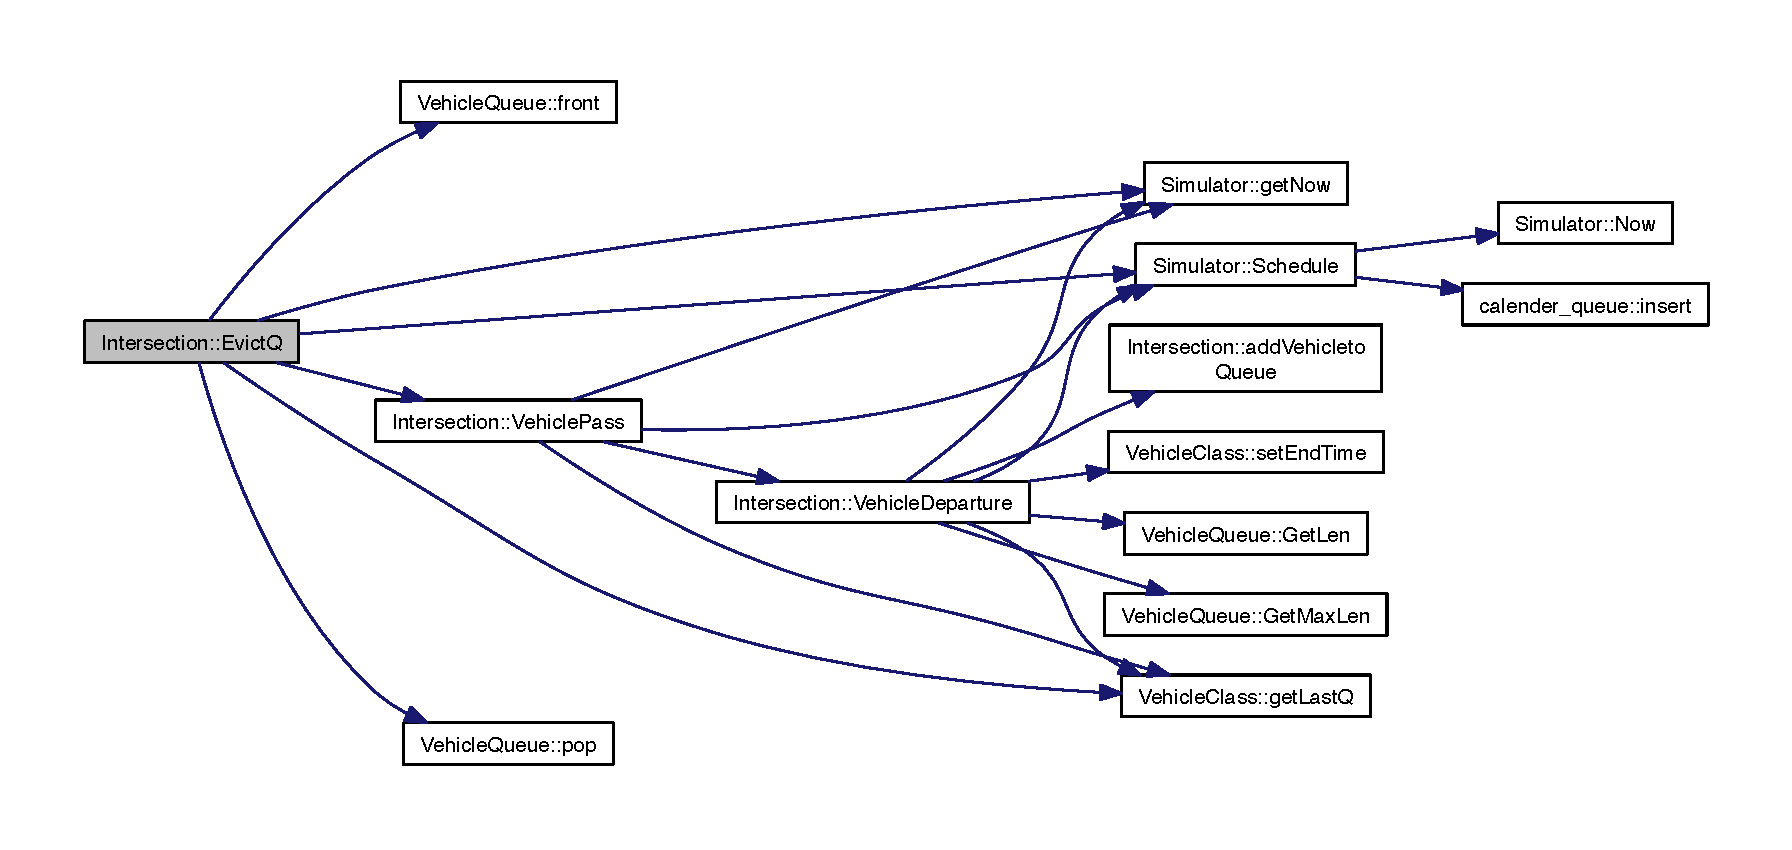
\includegraphics[width=350pt]{class_intersection_ab6a6b34e31effdf156c39dabf523e5e8_cgraph}
\end{center}
\end{figure}


\hypertarget{class_intersection_af9ffdb4a85d4b9250cc74936068f8d2d}{\index{Intersection@{Intersection}!get\-I\-D@{get\-I\-D}}
\index{get\-I\-D@{get\-I\-D}!Intersection@{Intersection}}
\subsubsection[{get\-I\-D}]{\setlength{\rightskip}{0pt plus 5cm}int Intersection\-::get\-I\-D (
\begin{DoxyParamCaption}
{}
\end{DoxyParamCaption}
)\hspace{0.3cm}{\ttfamily [inline]}}}\label{class_intersection_af9ffdb4a85d4b9250cc74936068f8d2d}
Returns the I\-D of the intersection \hypertarget{class_intersection_a9304a1e23bdcc495ff95c5195b81d947}{\index{Intersection@{Intersection}!get\-Qdirection@{get\-Qdirection}}
\index{get\-Qdirection@{get\-Qdirection}!Intersection@{Intersection}}
\subsubsection[{get\-Qdirection}]{\setlength{\rightskip}{0pt plus 5cm}int Intersection\-::get\-Qdirection (
\begin{DoxyParamCaption}
\item[{{\bf Intersection} $\ast$}]{inter, }
\item[{{\bf Vehicle\-Queue} $\ast$}]{Q}
\end{DoxyParamCaption}
)}}\label{class_intersection_a9304a1e23bdcc495ff95c5195b81d947}
Gets the direction of the queue \hypertarget{class_intersection_a2f76abb6014473396954bcaa0db18e7e}{\index{Intersection@{Intersection}!get\-Qlane@{get\-Qlane}}
\index{get\-Qlane@{get\-Qlane}!Intersection@{Intersection}}
\subsubsection[{get\-Qlane}]{\setlength{\rightskip}{0pt plus 5cm}int Intersection\-::get\-Qlane (
\begin{DoxyParamCaption}
\item[{{\bf Intersection} $\ast$}]{inter, }
\item[{{\bf Vehicle\-Queue} $\ast$}]{Q}
\end{DoxyParamCaption}
)}}\label{class_intersection_a2f76abb6014473396954bcaa0db18e7e}
Get the queue lane \hypertarget{class_intersection_a1cc47dcabbfb512f9cb85ff9e7114e1a}{\index{Intersection@{Intersection}!Next\-Q\-Info@{Next\-Q\-Info}}
\index{Next\-Q\-Info@{Next\-Q\-Info}!Intersection@{Intersection}}
\subsubsection[{Next\-Q\-Info}]{\setlength{\rightskip}{0pt plus 5cm}void Intersection\-::\-Next\-Q\-Info (
\begin{DoxyParamCaption}
\item[{{\bf Vehicle\-Queue} $\ast$}]{current\-Q, }
\item[{{\bf Vehicle\-Class} $\ast$}]{vehicle, }
\item[{{\bf Intersection} $\ast$\&}]{Next\-Inter, }
\item[{{\bf Vehicle\-Queue} $\ast$\&}]{Future\-Q, }
\item[{bool \&}]{isfull, }
\item[{int \&}]{Turn}
\end{DoxyParamCaption}
)}}\label{class_intersection_a1cc47dcabbfb512f9cb85ff9e7114e1a}
Gets the next queue info 

Here is the call graph for this function\-:\nopagebreak
\begin{figure}[H]
\begin{center}
\leavevmode
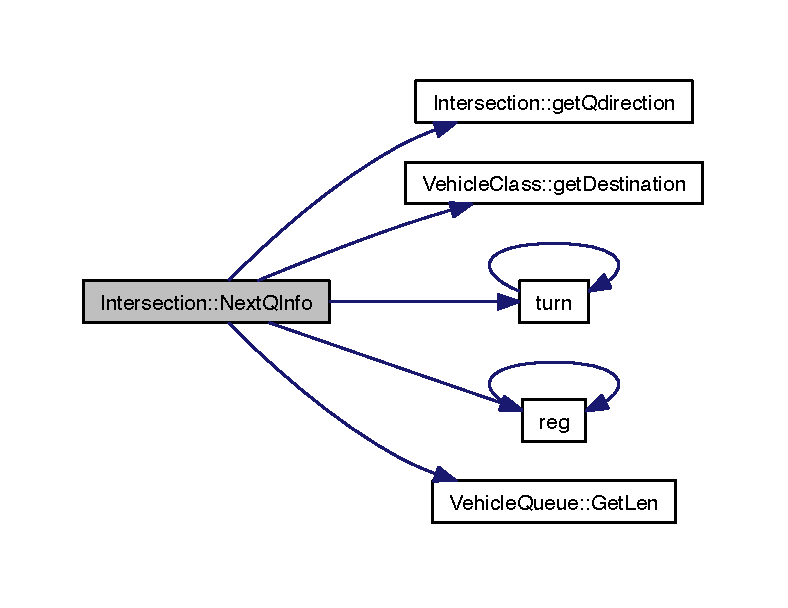
\includegraphics[width=350pt]{class_intersection_a1cc47dcabbfb512f9cb85ff9e7114e1a_cgraph}
\end{center}
\end{figure}


\hypertarget{class_intersection_ade54ec591355782db542061623096a2f}{\index{Intersection@{Intersection}!Q\-Can\-Go@{Q\-Can\-Go}}
\index{Q\-Can\-Go@{Q\-Can\-Go}!Intersection@{Intersection}}
\subsubsection[{Q\-Can\-Go}]{\setlength{\rightskip}{0pt plus 5cm}virtual int Intersection\-::\-Q\-Can\-Go (
\begin{DoxyParamCaption}
\item[{int}]{direction, }
\item[{int}]{lane}
\end{DoxyParamCaption}
)\hspace{0.3cm}{\ttfamily [pure virtual]}}}\label{class_intersection_ade54ec591355782db542061623096a2f}
Q\-C\-An\-Go 

Implemented in \hyperlink{class_intersectionwith_signal_a3b2a6f1e258fcd15828ffb7e9e9881b3}{Intersectionwith\-Signal}, and \hyperlink{class_intersectionwithout_signal_ac003b0651a33eb53986c4b0389f2c788}{Intersectionwithout\-Signal}.

\hypertarget{class_intersection_a358151a5ef4dd58dd42a6444c7e9bfc9}{\index{Intersection@{Intersection}!Vehicle\-Departure@{Vehicle\-Departure}}
\index{Vehicle\-Departure@{Vehicle\-Departure}!Intersection@{Intersection}}
\subsubsection[{Vehicle\-Departure}]{\setlength{\rightskip}{0pt plus 5cm}void Intersection\-::\-Vehicle\-Departure (
\begin{DoxyParamCaption}
\item[{{\bf Vehicle\-Class} $\ast$}]{vehicle}
\end{DoxyParamCaption}
)}}\label{class_intersection_a358151a5ef4dd58dd42a6444c7e9bfc9}
Departs Vehicle from the intersection 
\begin{DoxyParams}{Parameters}
{\em vehicle} & is the vehicle to be departed \\
\hline
\end{DoxyParams}


Here is the call graph for this function\-:
\nopagebreak
\begin{figure}[H]
\begin{center}
\leavevmode
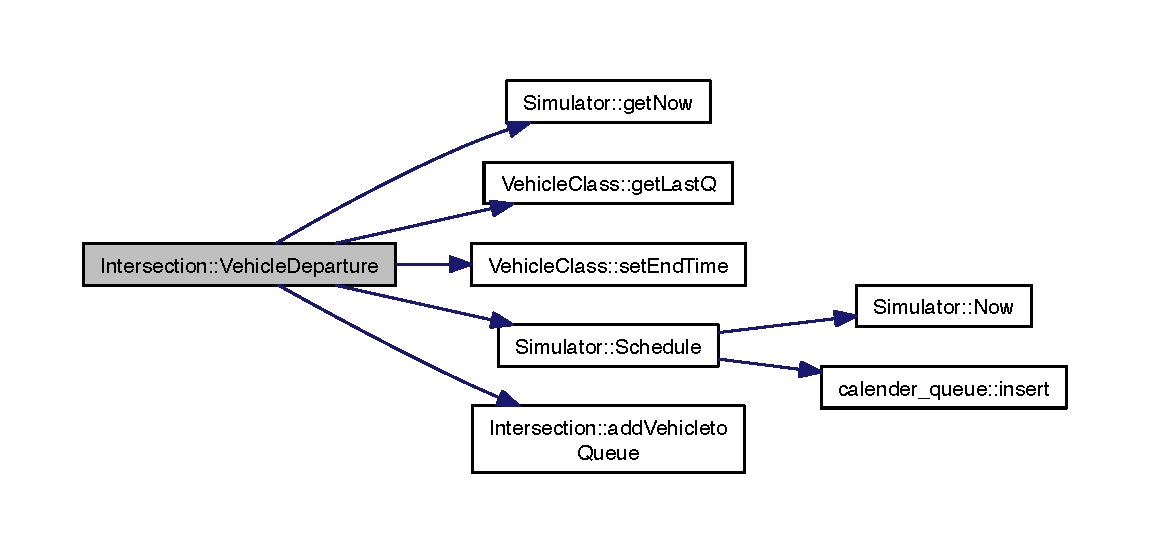
\includegraphics[width=350pt]{class_intersection_a358151a5ef4dd58dd42a6444c7e9bfc9_cgraph}
\end{center}
\end{figure}


\hypertarget{class_intersection_afe2e42381c4cf467fca7d2217d92524c}{\index{Intersection@{Intersection}!Vehicle\-Pass@{Vehicle\-Pass}}
\index{Vehicle\-Pass@{Vehicle\-Pass}!Intersection@{Intersection}}
\subsubsection[{Vehicle\-Pass}]{\setlength{\rightskip}{0pt plus 5cm}void Intersection\-::\-Vehicle\-Pass (
\begin{DoxyParamCaption}
\item[{{\bf Vehicle\-Class} $\ast$}]{vehicle, }
\item[{int}]{Turn}
\end{DoxyParamCaption}
)}}\label{class_intersection_afe2e42381c4cf467fca7d2217d92524c}
Logic of vehicle passing through this intersection 
\begin{DoxyParams}{Parameters}
{\em Vehicle} & \\
\hline
{\em turn} & \\
\hline
\end{DoxyParams}


Here is the call graph for this function\-:
\nopagebreak
\begin{figure}[H]
\begin{center}
\leavevmode
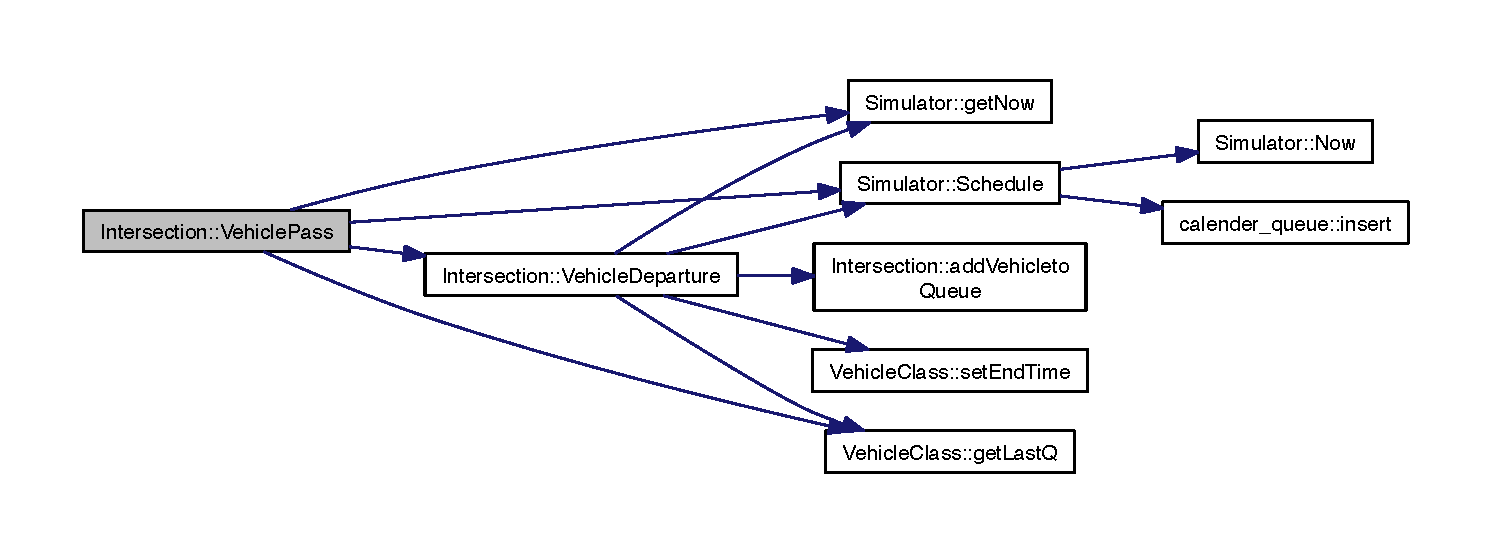
\includegraphics[width=350pt]{class_intersection_afe2e42381c4cf467fca7d2217d92524c_cgraph}
\end{center}
\end{figure}




\subsection{Member Data Documentation}
\hypertarget{class_intersection_ac7c8fd3e12e9df00670ae7c0f77d1e17}{\index{Intersection@{Intersection}!busy@{busy}}
\index{busy@{busy}!Intersection@{Intersection}}
\subsubsection[{busy}]{\setlength{\rightskip}{0pt plus 5cm}bool Intersection\-::busy\hspace{0.3cm}{\ttfamily [protected]}}}\label{class_intersection_ac7c8fd3e12e9df00670ae7c0f77d1e17}
Busy or not \hypertarget{class_intersection_a8a64af1004807f4ac451bcf9bfa368a4}{\index{Intersection@{Intersection}!E\-B\-I1@{E\-B\-I1}}
\index{E\-B\-I1@{E\-B\-I1}!Intersection@{Intersection}}
\subsubsection[{E\-B\-I1}]{\setlength{\rightskip}{0pt plus 5cm}{\bf Vehicle\-Queue}$\ast$ Intersection\-::\-E\-B\-I1}}\label{class_intersection_a8a64af1004807f4ac451bcf9bfa368a4}
Vehicle Queue East bound lane 1 \hypertarget{class_intersection_a8db85628804847f2b98fd1edf5c28e34}{\index{Intersection@{Intersection}!E\-B\-I2@{E\-B\-I2}}
\index{E\-B\-I2@{E\-B\-I2}!Intersection@{Intersection}}
\subsubsection[{E\-B\-I2}]{\setlength{\rightskip}{0pt plus 5cm}{\bf Vehicle\-Queue}$\ast$ Intersection\-::\-E\-B\-I2}}\label{class_intersection_a8db85628804847f2b98fd1edf5c28e34}
Vehicle Queue East bound lane 2 \hypertarget{class_intersection_a2456746faabd194633c2b133440449c6}{\index{Intersection@{Intersection}!Exit\-Q@{Exit\-Q}}
\index{Exit\-Q@{Exit\-Q}!Intersection@{Intersection}}
\subsubsection[{Exit\-Q}]{\setlength{\rightskip}{0pt plus 5cm}{\bf Vehicle\-Queue}$\ast$ Intersection\-::\-Exit\-Q}}\label{class_intersection_a2456746faabd194633c2b133440449c6}
all vehicle exiting the system are queued into Exit queue for post processing \hypertarget{class_intersection_a6c8f8ad77cc05de03282b613001a5729}{\index{Intersection@{Intersection}!have\-Signal@{have\-Signal}}
\index{have\-Signal@{have\-Signal}!Intersection@{Intersection}}
\subsubsection[{have\-Signal}]{\setlength{\rightskip}{0pt plus 5cm}bool Intersection\-::have\-Signal\hspace{0.3cm}{\ttfamily [protected]}}}\label{class_intersection_a6c8f8ad77cc05de03282b613001a5729}
Have traffic signal or not \hypertarget{class_intersection_aec0f4beb4f24b87b7f47aa6e23b7f4dd}{\index{Intersection@{Intersection}!I\-D@{I\-D}}
\index{I\-D@{I\-D}!Intersection@{Intersection}}
\subsubsection[{I\-D}]{\setlength{\rightskip}{0pt plus 5cm}int Intersection\-::\-I\-D\hspace{0.3cm}{\ttfamily [protected]}}}\label{class_intersection_aec0f4beb4f24b87b7f47aa6e23b7f4dd}
\hyperlink{class_intersection}{Intersection} Id \hypertarget{class_intersection_aba3182ae5b832420344bc8fccf5c285b}{\index{Intersection@{Intersection}!N\-B\-I1@{N\-B\-I1}}
\index{N\-B\-I1@{N\-B\-I1}!Intersection@{Intersection}}
\subsubsection[{N\-B\-I1}]{\setlength{\rightskip}{0pt plus 5cm}{\bf Vehicle\-Queue}$\ast$ Intersection\-::\-N\-B\-I1}}\label{class_intersection_aba3182ae5b832420344bc8fccf5c285b}
Vehicle Queue North bound lane 1 \hypertarget{class_intersection_af19480d80bcd05c9b3d6fff9e1e829d7}{\index{Intersection@{Intersection}!N\-B\-I2@{N\-B\-I2}}
\index{N\-B\-I2@{N\-B\-I2}!Intersection@{Intersection}}
\subsubsection[{N\-B\-I2}]{\setlength{\rightskip}{0pt plus 5cm}{\bf Vehicle\-Queue}$\ast$ Intersection\-::\-N\-B\-I2}}\label{class_intersection_af19480d80bcd05c9b3d6fff9e1e829d7}
Vehicle Queue North bound lane 2 \hypertarget{class_intersection_a577edea4aa08d05052e6cbf7aa2ba9e2}{\index{Intersection@{Intersection}!N\-Inter@{N\-Inter}}
\index{N\-Inter@{N\-Inter}!Intersection@{Intersection}}
\subsubsection[{N\-Inter}]{\setlength{\rightskip}{0pt plus 5cm}{\bf Intersection}$\ast$ Intersection\-::\-N\-Inter}}\label{class_intersection_a577edea4aa08d05052e6cbf7aa2ba9e2}
Neighboring intersection in the North \hypertarget{class_intersection_a87a7802a02ff65c92a6fd11c70144ca2}{\index{Intersection@{Intersection}!routingtable@{routingtable}}
\index{routingtable@{routingtable}!Intersection@{Intersection}}
\subsubsection[{routingtable}]{\setlength{\rightskip}{0pt plus 5cm}dir Intersection\-::routingtable\mbox{[}12\mbox{]}}}\label{class_intersection_a87a7802a02ff65c92a6fd11c70144ca2}
Acts as trnslator for routing cars \hypertarget{class_intersection_a0f60a7d5b4911fbc309ddecdab4a75e7}{\index{Intersection@{Intersection}!S\-B\-I1@{S\-B\-I1}}
\index{S\-B\-I1@{S\-B\-I1}!Intersection@{Intersection}}
\subsubsection[{S\-B\-I1}]{\setlength{\rightskip}{0pt plus 5cm}{\bf Vehicle\-Queue}$\ast$ Intersection\-::\-S\-B\-I1}}\label{class_intersection_a0f60a7d5b4911fbc309ddecdab4a75e7}
Vehicle Queue South bound lane 1 \hypertarget{class_intersection_a172b271e9434b824c4722b1589d77f55}{\index{Intersection@{Intersection}!S\-B\-I2@{S\-B\-I2}}
\index{S\-B\-I2@{S\-B\-I2}!Intersection@{Intersection}}
\subsubsection[{S\-B\-I2}]{\setlength{\rightskip}{0pt plus 5cm}{\bf Vehicle\-Queue}$\ast$ Intersection\-::\-S\-B\-I2}}\label{class_intersection_a172b271e9434b824c4722b1589d77f55}
Vehicle Queue South bound lane 2 \hypertarget{class_intersection_af6cfb23dbc2ad5b1d90752247dd07acf}{\index{Intersection@{Intersection}!S\-Inter@{S\-Inter}}
\index{S\-Inter@{S\-Inter}!Intersection@{Intersection}}
\subsubsection[{S\-Inter}]{\setlength{\rightskip}{0pt plus 5cm}{\bf Intersection}$\ast$ Intersection\-::\-S\-Inter}}\label{class_intersection_af6cfb23dbc2ad5b1d90752247dd07acf}
Neighboring intersection in the South \hypertarget{class_intersection_a7d4afb62f4051e6f25c0195de1d66442}{\index{Intersection@{Intersection}!W\-B\-I1@{W\-B\-I1}}
\index{W\-B\-I1@{W\-B\-I1}!Intersection@{Intersection}}
\subsubsection[{W\-B\-I1}]{\setlength{\rightskip}{0pt plus 5cm}{\bf Vehicle\-Queue}$\ast$ Intersection\-::\-W\-B\-I1}}\label{class_intersection_a7d4afb62f4051e6f25c0195de1d66442}
Vehicle Queue West bound lane 1 \hypertarget{class_intersection_a7f4c7a9c2344827a24aaa52955e56fac}{\index{Intersection@{Intersection}!W\-B\-I2@{W\-B\-I2}}
\index{W\-B\-I2@{W\-B\-I2}!Intersection@{Intersection}}
\subsubsection[{W\-B\-I2}]{\setlength{\rightskip}{0pt plus 5cm}{\bf Vehicle\-Queue}$\ast$ Intersection\-::\-W\-B\-I2}}\label{class_intersection_a7f4c7a9c2344827a24aaa52955e56fac}
Vehicle Queue West bound lane 2 

The documentation for this class was generated from the following files\-:\begin{DoxyCompactItemize}
\item 
\hyperlink{_intersection_8h}{Intersection.\-h}\item 
Intersection.\-cpp\end{DoxyCompactItemize}

\hypertarget{class_intersectionwithout_signal}{\section{Intersectionwithout\-Signal Class Reference}
\label{class_intersectionwithout_signal}\index{Intersectionwithout\-Signal@{Intersectionwithout\-Signal}}
}


Inheritance diagram for Intersectionwithout\-Signal\-:\nopagebreak
\begin{figure}[H]
\begin{center}
\leavevmode
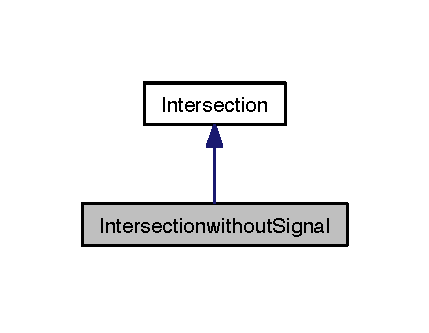
\includegraphics[width=206pt]{class_intersectionwithout_signal__inherit__graph}
\end{center}
\end{figure}


Collaboration diagram for Intersectionwithout\-Signal\-:\nopagebreak
\begin{figure}[H]
\begin{center}
\leavevmode
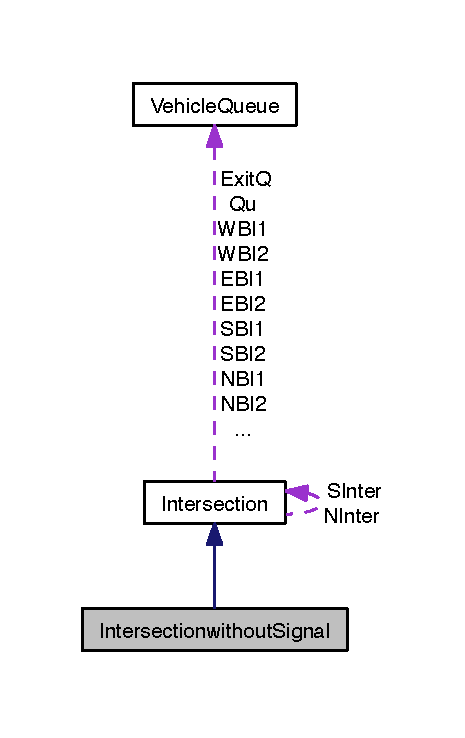
\includegraphics[width=223pt]{class_intersectionwithout_signal__coll__graph}
\end{center}
\end{figure}
\subsection*{Public Member Functions}
\begin{DoxyCompactItemize}
\item 
\hypertarget{class_intersectionwithout_signal_ab538d75fb2afe614867754e0debbd2e2}{virtual void {\bfseries add\-Vehicleto\-Queue} (\hyperlink{class_vehicle_queue}{Vehicle\-Queue} $\ast$joinqueue, \hyperlink{class_vehicle_class}{Vehicle\-Class} $\ast$vehicle)}\label{class_intersectionwithout_signal_ab538d75fb2afe614867754e0debbd2e2}

\item 
\hypertarget{class_intersectionwithout_signal_ac003b0651a33eb53986c4b0389f2c788}{virtual int {\bfseries Q\-Can\-Go} (int direction, int lane)}\label{class_intersectionwithout_signal_ac003b0651a33eb53986c4b0389f2c788}

\item 
\hypertarget{class_intersectionwithout_signal_a7afe1b9d80f5424b5cb36448245b3453}{{\bfseries Intersectionwithout\-Signal} (int)}\label{class_intersectionwithout_signal_a7afe1b9d80f5424b5cb36448245b3453}

\end{DoxyCompactItemize}
\subsection*{Additional Inherited Members}


The documentation for this class was generated from the following files\-:\begin{DoxyCompactItemize}
\item 
Intersectionwo\-Signal.\-h\item 
Intersectionwo\-Signal.\-cpp\end{DoxyCompactItemize}

\hypertarget{class_intersectionwith_signal}{\section{Intersectionwith\-Signal Class Reference}
\label{class_intersectionwith_signal}\index{Intersectionwith\-Signal@{Intersectionwith\-Signal}}
}


Inheritance diagram for Intersectionwith\-Signal\-:\nopagebreak
\begin{figure}[H]
\begin{center}
\leavevmode
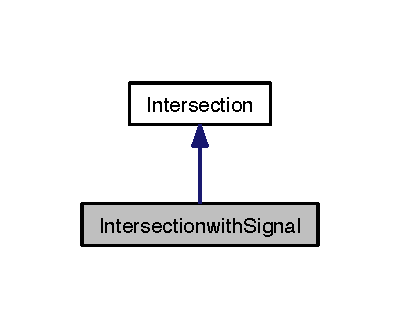
\includegraphics[width=192pt]{class_intersectionwith_signal__inherit__graph}
\end{center}
\end{figure}


Collaboration diagram for Intersectionwith\-Signal\-:\nopagebreak
\begin{figure}[H]
\begin{center}
\leavevmode
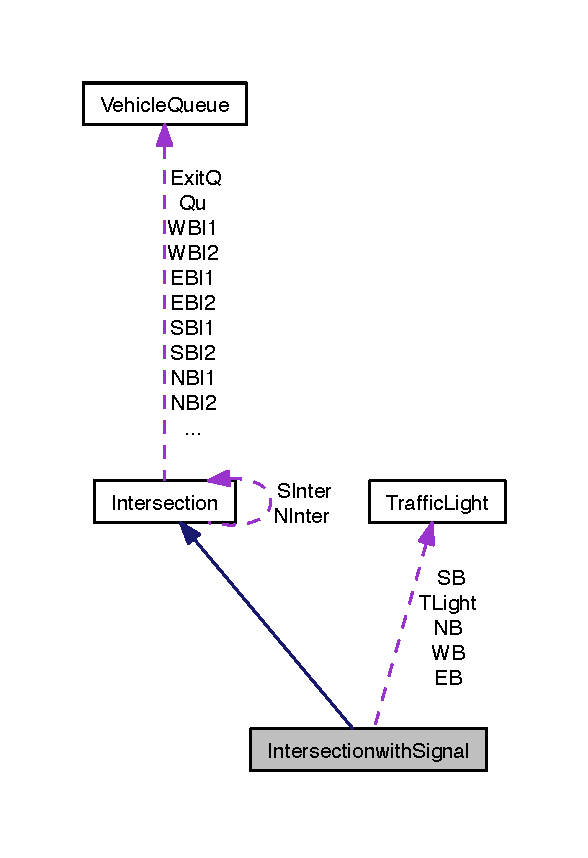
\includegraphics[width=282pt]{class_intersectionwith_signal__coll__graph}
\end{center}
\end{figure}
\subsection*{Public Member Functions}
\begin{DoxyCompactItemize}
\item 
\hypertarget{class_intersectionwith_signal_a7fa2f6aa47aa7624c483523a920d92a4}{void {\bfseries change\-Signal\-Trigger} (int Light\-I\-D)}\label{class_intersectionwith_signal_a7fa2f6aa47aa7624c483523a920d92a4}

\item 
\hypertarget{class_intersectionwith_signal_aa918c9a3033c16fac6bfa0e996677670}{virtual void {\bfseries add\-Vehicleto\-Queue} (\hyperlink{class_vehicle_queue}{Vehicle\-Queue} $\ast$joinqueue, \hyperlink{class_vehicle_class}{Vehicle\-Class} $\ast$vehicle)}\label{class_intersectionwith_signal_aa918c9a3033c16fac6bfa0e996677670}

\item 
\hypertarget{class_intersectionwith_signal_a3b2a6f1e258fcd15828ffb7e9e9881b3}{virtual int {\bfseries Q\-Can\-Go} (int direction, int lane)}\label{class_intersectionwith_signal_a3b2a6f1e258fcd15828ffb7e9e9881b3}

\item 
\hypertarget{class_intersectionwith_signal_ab5eccdd602e1d9c0f6d39b5be79173d1}{{\bfseries Intersectionwith\-Signal} (int)}\label{class_intersectionwith_signal_ab5eccdd602e1d9c0f6d39b5be79173d1}

\end{DoxyCompactItemize}
\subsection*{Public Attributes}
\begin{DoxyCompactItemize}
\item 
\hypertarget{class_intersectionwith_signal_a8a57308329169b7c05acdeabfaa74206}{\hyperlink{class_traffic_light}{Traffic\-Light} $\ast$ {\bfseries E\-B}}\label{class_intersectionwith_signal_a8a57308329169b7c05acdeabfaa74206}

\item 
\hypertarget{class_intersectionwith_signal_a5f321e72c10bb5a4ebeb6d314135fdbb}{\hyperlink{class_traffic_light}{Traffic\-Light} $\ast$ {\bfseries W\-B}}\label{class_intersectionwith_signal_a5f321e72c10bb5a4ebeb6d314135fdbb}

\item 
\hypertarget{class_intersectionwith_signal_af548458cb3fbe82d25a13fd9295406f7}{\hyperlink{class_traffic_light}{Traffic\-Light} $\ast$ {\bfseries N\-B}}\label{class_intersectionwith_signal_af548458cb3fbe82d25a13fd9295406f7}

\item 
\hypertarget{class_intersectionwith_signal_a19a6f5316f7d0ec4c08e6f80126b3e6c}{\hyperlink{class_traffic_light}{Traffic\-Light} $\ast$ {\bfseries S\-B}}\label{class_intersectionwith_signal_a19a6f5316f7d0ec4c08e6f80126b3e6c}

\item 
\hypertarget{class_intersectionwith_signal_a2c5e8c7432419eac922f8efa01a2f487}{\hyperlink{class_traffic_light}{Traffic\-Light} $\ast$ {\bfseries T\-Light} \mbox{[}4\mbox{]}}\label{class_intersectionwith_signal_a2c5e8c7432419eac922f8efa01a2f487}

\end{DoxyCompactItemize}
\subsection*{Additional Inherited Members}


The documentation for this class was generated from the following files\-:\begin{DoxyCompactItemize}
\item 
Intersectionwith\-Signal.\-h\item 
Intersectionwith\-Signal.\-cpp\end{DoxyCompactItemize}

\hypertarget{classprioqueue}{\section{prioqueue Class Reference}
\label{classprioqueue}\index{prioqueue@{prioqueue}}
}
\subsection*{Public Member Functions}
\begin{DoxyCompactItemize}
\item 
\hypertarget{classprioqueue_a1d26a2fefd8d30b3c92d0e449c330625}{void {\bfseries enqueue} (\hyperlink{class_event_base}{Event\-Base} $\ast$)}\label{classprioqueue_a1d26a2fefd8d30b3c92d0e449c330625}

\item 
\hypertarget{classprioqueue_ab0920a604ff20b46980b2d10428aff06}{\hyperlink{class_event_base}{Event\-Base} $\ast$ {\bfseries dequeue} (\hyperlink{class_event_base}{Event\-Base} $\ast$)}\label{classprioqueue_ab0920a604ff20b46980b2d10428aff06}

\item 
\hypertarget{classprioqueue_a38aa9bcfe969f527fe70e8e37c1807b1}{\hyperlink{class_event_base}{Event\-Base} $\ast$ {\bfseries Pop\-Next} ()}\label{classprioqueue_a38aa9bcfe969f527fe70e8e37c1807b1}

\item 
\hypertarget{classprioqueue_aaa9d01e19413c4d7fa957d5ac2a7b705}{bool {\bfseries is\-Empty} ()}\label{classprioqueue_aaa9d01e19413c4d7fa957d5ac2a7b705}

\end{DoxyCompactItemize}


The documentation for this class was generated from the following file\-:\begin{DoxyCompactItemize}
\item 
prioqueue.\-h\end{DoxyCompactItemize}

\hypertarget{class_random_num_gen}{\section{Random\-Num\-Gen Class Reference}
\label{class_random_num_gen}\index{Random\-Num\-Gen@{Random\-Num\-Gen}}
}
\subsection*{Public Member Functions}
\begin{DoxyCompactItemize}
\item 
\hyperlink{class_random_num_gen_adc07d95ae2d1d3a5a4a395f233e30a2c}{Random\-Num\-Gen} ()
\item 
\hyperlink{class_random_num_gen_ac98ff22efa3b9c23e6b6ba1cf6a6097f}{Random\-Num\-Gen} (unsigned long x0)
\item 
double \hyperlink{class_random_num_gen_a49782fde536ad4b01ab3bd6063a5c6c2}{Next} ()
\item 
void \hyperlink{class_random_num_gen_a12e515fdf02cd66772a76ae0765d4d08}{Reset} ()
\item 
unsigned long \hyperlink{class_random_num_gen_a936200dd149f676875efaa2dbed8699e}{Get\-State} ()
\item 
\hyperlink{class_random_num_gen_a8fec599a61c18b20bfd567ff5b80ab31}{$\sim$\-Random\-Num\-Gen} ()
\end{DoxyCompactItemize}


\subsection{Constructor \& Destructor Documentation}
\hypertarget{class_random_num_gen_adc07d95ae2d1d3a5a4a395f233e30a2c}{\index{Random\-Num\-Gen@{Random\-Num\-Gen}!Random\-Num\-Gen@{Random\-Num\-Gen}}
\index{Random\-Num\-Gen@{Random\-Num\-Gen}!RandomNumGen@{Random\-Num\-Gen}}
\subsubsection[{Random\-Num\-Gen}]{\setlength{\rightskip}{0pt plus 5cm}Random\-Num\-Gen\-::\-Random\-Num\-Gen (
\begin{DoxyParamCaption}
{}
\end{DoxyParamCaption}
)}}\label{class_random_num_gen_adc07d95ae2d1d3a5a4a395f233e30a2c}
Constructor\-: Initializes the default parameters of Random number genrator \hypertarget{class_random_num_gen_ac98ff22efa3b9c23e6b6ba1cf6a6097f}{\index{Random\-Num\-Gen@{Random\-Num\-Gen}!Random\-Num\-Gen@{Random\-Num\-Gen}}
\index{Random\-Num\-Gen@{Random\-Num\-Gen}!RandomNumGen@{Random\-Num\-Gen}}
\subsubsection[{Random\-Num\-Gen}]{\setlength{\rightskip}{0pt plus 5cm}Random\-Num\-Gen\-::\-Random\-Num\-Gen (
\begin{DoxyParamCaption}
\item[{unsigned long}]{x0}
\end{DoxyParamCaption}
)}}\label{class_random_num_gen_ac98ff22efa3b9c23e6b6ba1cf6a6097f}
Constuctor\-: Initializes the starting state with x0 
\begin{DoxyParams}{Parameters}
{\em x0} & is long input, if 0 takes starting point seed as time, otherwise sets x0 as the internal state \\
\hline
\end{DoxyParams}


Here is the call graph for this function\-:
\nopagebreak
\begin{figure}[H]
\begin{center}
\leavevmode
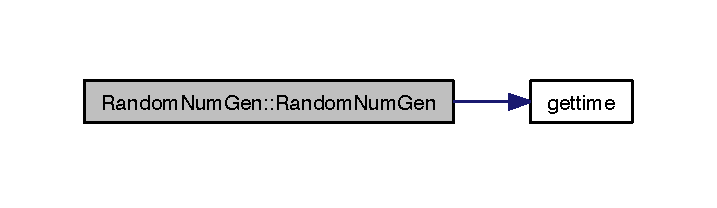
\includegraphics[width=344pt]{class_random_num_gen_ac98ff22efa3b9c23e6b6ba1cf6a6097f_cgraph}
\end{center}
\end{figure}


\hypertarget{class_random_num_gen_a8fec599a61c18b20bfd567ff5b80ab31}{\index{Random\-Num\-Gen@{Random\-Num\-Gen}!$\sim$\-Random\-Num\-Gen@{$\sim$\-Random\-Num\-Gen}}
\index{$\sim$\-Random\-Num\-Gen@{$\sim$\-Random\-Num\-Gen}!RandomNumGen@{Random\-Num\-Gen}}
\subsubsection[{$\sim$\-Random\-Num\-Gen}]{\setlength{\rightskip}{0pt plus 5cm}Random\-Num\-Gen\-::$\sim$\-Random\-Num\-Gen (
\begin{DoxyParamCaption}
{}
\end{DoxyParamCaption}
)}}\label{class_random_num_gen_a8fec599a61c18b20bfd567ff5b80ab31}
Destructor for random number genrator 

\subsection{Member Function Documentation}
\hypertarget{class_random_num_gen_a936200dd149f676875efaa2dbed8699e}{\index{Random\-Num\-Gen@{Random\-Num\-Gen}!Get\-State@{Get\-State}}
\index{Get\-State@{Get\-State}!RandomNumGen@{Random\-Num\-Gen}}
\subsubsection[{Get\-State}]{\setlength{\rightskip}{0pt plus 5cm}unsigned long Random\-Num\-Gen\-::\-Get\-State (
\begin{DoxyParamCaption}
{}
\end{DoxyParamCaption}
)}}\label{class_random_num_gen_a936200dd149f676875efaa2dbed8699e}
Gives state of random genrator. Used for debugging purpose \hypertarget{class_random_num_gen_a49782fde536ad4b01ab3bd6063a5c6c2}{\index{Random\-Num\-Gen@{Random\-Num\-Gen}!Next@{Next}}
\index{Next@{Next}!RandomNumGen@{Random\-Num\-Gen}}
\subsubsection[{Next}]{\setlength{\rightskip}{0pt plus 5cm}double Random\-Num\-Gen\-::\-Next (
\begin{DoxyParamCaption}
{}
\end{DoxyParamCaption}
)}}\label{class_random_num_gen_a49782fde536ad4b01ab3bd6063a5c6c2}
Genrates next random number \hypertarget{class_random_num_gen_a12e515fdf02cd66772a76ae0765d4d08}{\index{Random\-Num\-Gen@{Random\-Num\-Gen}!Reset@{Reset}}
\index{Reset@{Reset}!RandomNumGen@{Random\-Num\-Gen}}
\subsubsection[{Reset}]{\setlength{\rightskip}{0pt plus 5cm}void Random\-Num\-Gen\-::\-Reset (
\begin{DoxyParamCaption}
{}
\end{DoxyParamCaption}
)}}\label{class_random_num_gen_a12e515fdf02cd66772a76ae0765d4d08}
Resets the random number generator 

The documentation for this class was generated from the following files\-:\begin{DoxyCompactItemize}
\item 
\hyperlink{_random_num_8h}{Random\-Num.\-h}\item 
\hyperlink{_random_num_8cc}{Random\-Num.\-cc}\end{DoxyCompactItemize}

\hypertarget{class_road_segment}{\section{Road\-Segment Class Reference}
\label{class_road_segment}\index{Road\-Segment@{Road\-Segment}}
}


Collaboration diagram for Road\-Segment\-:\nopagebreak
\begin{figure}[H]
\begin{center}
\leavevmode
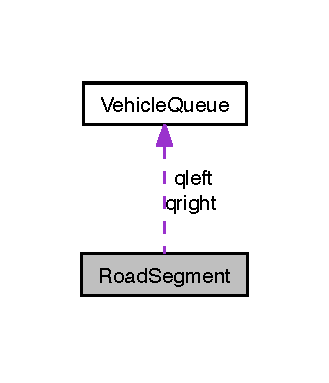
\includegraphics[width=158pt]{class_road_segment__coll__graph}
\end{center}
\end{figure}
\subsection*{Public Member Functions}
\begin{DoxyCompactItemize}
\item 
\hyperlink{class_road_segment_ab7caf1e5f213f7584687edce88a17cdd}{Road\-Segment} (dir direction, \hyperlink{class_intersection}{Intersection} $\ast$par, int cap)
\item 
void \hyperlink{class_road_segment_a86d7460856feadb6faa86e130b090479}{Add\-Vehicle} (\hyperlink{class_vehicle_class}{Vehicle\-Class} $\ast$vehicle)
\item 
void \hyperlink{class_road_segment_a9ca3951ccd16a925d6aad11ff97f6591}{Evict\-Vehicle} ()
\end{DoxyCompactItemize}
\subsection*{Public Attributes}
\begin{DoxyCompactItemize}
\item 
\hyperlink{class_vehicle_queue}{Vehicle\-Queue} \hyperlink{class_road_segment_a33e663e38e3d1944398ff70198fdb77b}{qright}
\item 
\hyperlink{class_vehicle_queue}{Vehicle\-Queue} \hyperlink{class_road_segment_a0272daa14fc04bc471f81409db27b80b}{qleft}
\end{DoxyCompactItemize}


\subsection{Constructor \& Destructor Documentation}
\hypertarget{class_road_segment_ab7caf1e5f213f7584687edce88a17cdd}{\index{Road\-Segment@{Road\-Segment}!Road\-Segment@{Road\-Segment}}
\index{Road\-Segment@{Road\-Segment}!RoadSegment@{Road\-Segment}}
\subsubsection[{Road\-Segment}]{\setlength{\rightskip}{0pt plus 5cm}Road\-Segment\-::\-Road\-Segment (
\begin{DoxyParamCaption}
\item[{dir}]{direction, }
\item[{{\bf Intersection} $\ast$}]{par, }
\item[{int}]{cap}
\end{DoxyParamCaption}
)\hspace{0.3cm}{\ttfamily [inline]}}}\label{class_road_segment_ab7caf1e5f213f7584687edce88a17cdd}
Constructor 

\subsection{Member Function Documentation}
\hypertarget{class_road_segment_a86d7460856feadb6faa86e130b090479}{\index{Road\-Segment@{Road\-Segment}!Add\-Vehicle@{Add\-Vehicle}}
\index{Add\-Vehicle@{Add\-Vehicle}!RoadSegment@{Road\-Segment}}
\subsubsection[{Add\-Vehicle}]{\setlength{\rightskip}{0pt plus 5cm}void Road\-Segment\-::\-Add\-Vehicle (
\begin{DoxyParamCaption}
\item[{{\bf Vehicle\-Class} $\ast$}]{vehicle}
\end{DoxyParamCaption}
)}}\label{class_road_segment_a86d7460856feadb6faa86e130b090479}
Adds vehicle to the road segment 

Here is the call graph for this function\-:\nopagebreak
\begin{figure}[H]
\begin{center}
\leavevmode
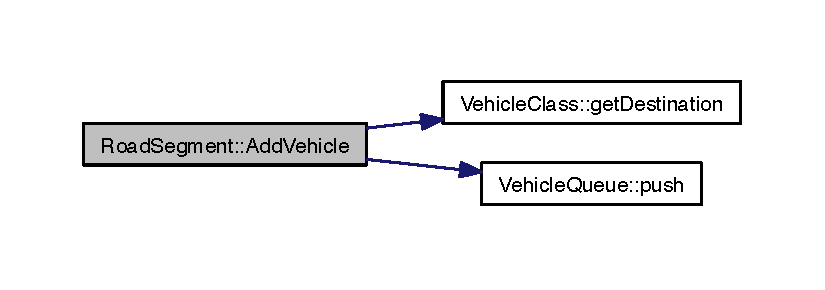
\includegraphics[width=350pt]{class_road_segment_a86d7460856feadb6faa86e130b090479_cgraph}
\end{center}
\end{figure}


\hypertarget{class_road_segment_a9ca3951ccd16a925d6aad11ff97f6591}{\index{Road\-Segment@{Road\-Segment}!Evict\-Vehicle@{Evict\-Vehicle}}
\index{Evict\-Vehicle@{Evict\-Vehicle}!RoadSegment@{Road\-Segment}}
\subsubsection[{Evict\-Vehicle}]{\setlength{\rightskip}{0pt plus 5cm}void Road\-Segment\-::\-Evict\-Vehicle (
\begin{DoxyParamCaption}
{}
\end{DoxyParamCaption}
)}}\label{class_road_segment_a9ca3951ccd16a925d6aad11ff97f6591}
Evicts vehicle from the Road Segment 

\subsection{Member Data Documentation}
\hypertarget{class_road_segment_a0272daa14fc04bc471f81409db27b80b}{\index{Road\-Segment@{Road\-Segment}!qleft@{qleft}}
\index{qleft@{qleft}!RoadSegment@{Road\-Segment}}
\subsubsection[{qleft}]{\setlength{\rightskip}{0pt plus 5cm}{\bf Vehicle\-Queue} Road\-Segment\-::qleft}}\label{class_road_segment_a0272daa14fc04bc471f81409db27b80b}
Left lane (Vehicle Queue) \hypertarget{class_road_segment_a33e663e38e3d1944398ff70198fdb77b}{\index{Road\-Segment@{Road\-Segment}!qright@{qright}}
\index{qright@{qright}!RoadSegment@{Road\-Segment}}
\subsubsection[{qright}]{\setlength{\rightskip}{0pt plus 5cm}{\bf Vehicle\-Queue} Road\-Segment\-::qright}}\label{class_road_segment_a33e663e38e3d1944398ff70198fdb77b}
Right lane (Vehicle queue) 

The documentation for this class was generated from the following files\-:\begin{DoxyCompactItemize}
\item 
\hyperlink{_road_segment_8h}{Road\-Segment.\-h}\item 
Road\-Segment.\-cpp\end{DoxyCompactItemize}

\hypertarget{class_simulator}{\section{Simulator Class Reference}
\label{class_simulator}\index{Simulator@{Simulator}}
}


Collaboration diagram for Simulator\-:\nopagebreak
\begin{figure}[H]
\begin{center}
\leavevmode
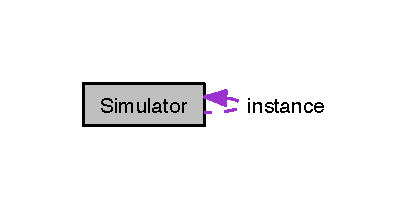
\includegraphics[width=196pt]{class_simulator__coll__graph}
\end{center}
\end{figure}
\subsection*{Public Member Functions}
\begin{DoxyCompactItemize}
\item 
\hypertarget{class_simulator_ad493423e80256f53c715bb59c16ec78e}{void {\bfseries Stop} ()}\label{class_simulator_ad493423e80256f53c715bb59c16ec78e}

\item 
\hypertarget{class_simulator_a7fe5c584b3fc3f93f5b13e882ca27009}{Time\-\_\-t {\bfseries get\-Now} ()}\label{class_simulator_a7fe5c584b3fc3f93f5b13e882ca27009}

\item 
\hypertarget{class_simulator_a0d67931f9d55c1f284f6467b9015c1c4}{{\footnotesize template$<$typename T , typename O\-B\-J , typename U1 , typename T1 $>$ }\\void {\bfseries Schedule} (double t, void(T\-::$\ast$handler)(U1), O\-B\-J $\ast$obj, T1 t1)}\label{class_simulator_a0d67931f9d55c1f284f6467b9015c1c4}

\item 
\hypertarget{class_simulator_a5dc207907f17173964ca9a04d7d4b8fe}{{\footnotesize template$<$typename T , typename O\-B\-J , typename U1 , typename T1 , typename U2 , typename T2 $>$ }\\void {\bfseries Schedule} (double t, void(T\-::$\ast$handler)(U1, U2), O\-B\-J $\ast$obj, T1 t1, T2 t2)}\label{class_simulator_a5dc207907f17173964ca9a04d7d4b8fe}

\item 
\hypertarget{class_simulator_a2a00f7c57e142e06046f4df091f0173b}{{\footnotesize template$<$typename T , typename O\-B\-J , typename U1 , typename T1 , typename U2 , typename T2 , typename U3 , typename T3 $>$ }\\void {\bfseries Schedule} (double t, void(T\-::$\ast$handler)(U1, U2, U3), O\-B\-J $\ast$obj, T1 t1, T2 t2, T3 t3)}\label{class_simulator_a2a00f7c57e142e06046f4df091f0173b}

\end{DoxyCompactItemize}
\subsection*{Static Public Member Functions}
\begin{DoxyCompactItemize}
\item 
\hypertarget{class_simulator_a27e7045e7aa4e29e9d2003aaa09c8326}{static void {\bfseries Run} ()}\label{class_simulator_a27e7045e7aa4e29e9d2003aaa09c8326}

\item 
\hypertarget{class_simulator_a4bbb179ecbac8adfee23bd49d19746c0}{static void {\bfseries Stop\-At} (Time\-\_\-t)}\label{class_simulator_a4bbb179ecbac8adfee23bd49d19746c0}

\item 
\hypertarget{class_simulator_ae9f1c5a28f2fc0d42ccead5d7d2a642d}{{\footnotesize template$<$typename T , typename O\-B\-J $>$ }\\static void {\bfseries Schedule} (double t, void(T\-::$\ast$handler)(void), O\-B\-J $\ast$obj)}\label{class_simulator_ae9f1c5a28f2fc0d42ccead5d7d2a642d}

\item 
\hypertarget{class_simulator_a4a9507b155c22a9c5f119abb2d2d6fc1}{static Time\-\_\-t {\bfseries Now} ()}\label{class_simulator_a4a9507b155c22a9c5f119abb2d2d6fc1}

\end{DoxyCompactItemize}
\subsection*{Static Public Attributes}
\begin{DoxyCompactItemize}
\item 
\hypertarget{class_simulator_a12033735d8c6b88db2aaf72113481f97}{static \hyperlink{class_simulator}{Simulator} $\ast$ {\bfseries instance} =0}\label{class_simulator_a12033735d8c6b88db2aaf72113481f97}

\end{DoxyCompactItemize}


The documentation for this class was generated from the following files\-:\begin{DoxyCompactItemize}
\item 
Simulator.\-h\item 
Simulator.\-cpp\end{DoxyCompactItemize}

\hypertarget{class_traffic_light}{\section{Traffic\-Light Class Reference}
\label{class_traffic_light}\index{Traffic\-Light@{Traffic\-Light}}
}
\subsection*{Public Member Functions}
\begin{DoxyCompactItemize}
\item 
\hypertarget{class_traffic_light_abce2ada7d1eeb16437d07acd50b2446b}{int {\bfseries get\-Type} ()}\label{class_traffic_light_abce2ada7d1eeb16437d07acd50b2446b}

\item 
\hypertarget{class_traffic_light_aaee73cd4cff5ad4f7096c7c8e9e6bc4b}{state {\bfseries get\-State} ()}\label{class_traffic_light_aaee73cd4cff5ad4f7096c7c8e9e6bc4b}

\item 
\hypertarget{class_traffic_light_ad3bb62de50352123ffa6d67b4cbd028f}{{\bfseries Traffic\-Light} (int id, int typ, state initial\-State, double Ph1, double Ph2, double Ph3, double Ph4, double Ph5, double Ph6, \hyperlink{class_intersectionwith_signal}{Intersectionwith\-Signal} $\ast$p)}\label{class_traffic_light_ad3bb62de50352123ffa6d67b4cbd028f}

\item 
\hypertarget{class_traffic_light_a069a58acd9a0b2ecb9245912b53c4462}{void {\bfseries cyclestate} ()}\label{class_traffic_light_a069a58acd9a0b2ecb9245912b53c4462}

\end{DoxyCompactItemize}
\subsection*{Public Attributes}
\begin{DoxyCompactItemize}
\item 
\hypertarget{class_traffic_light_aa8b8852f0a75b737d741cdb831847208}{int {\bfseries myid}}\label{class_traffic_light_aa8b8852f0a75b737d741cdb831847208}

\end{DoxyCompactItemize}


The documentation for this class was generated from the following files\-:\begin{DoxyCompactItemize}
\item 
Traffic\-Light.\-h\item 
Traffic\-Light.\-cpp\end{DoxyCompactItemize}

\hypertarget{class_vehicle_class}{\section{Vehicle\-Class Class Reference}
\label{class_vehicle_class}\index{Vehicle\-Class@{Vehicle\-Class}}
}
\subsection*{Public Member Functions}
\begin{DoxyCompactItemize}
\item 
\hypertarget{class_vehicle_class_a127372b94980fa045c648af412856fd5}{void {\bfseries set\-End\-Time} (Time\-\_\-t t)}\label{class_vehicle_class_a127372b94980fa045c648af412856fd5}

\item 
\hypertarget{class_vehicle_class_a8f00863bdcac1822d486c3d119ff1340}{int {\bfseries get\-I\-D} ()}\label{class_vehicle_class_a8f00863bdcac1822d486c3d119ff1340}

\item 
\hypertarget{class_vehicle_class_a7070e6f4e7814a6f81292a54aa3c58b5}{void \hyperlink{class_vehicle_class_a7070e6f4e7814a6f81292a54aa3c58b5}{update\-Direction} (dir Direction)}\label{class_vehicle_class_a7070e6f4e7814a6f81292a54aa3c58b5}

\begin{DoxyCompactList}\small\item\em !\-Constructor \end{DoxyCompactList}\item 
\hypertarget{class_vehicle_class_a107f9787110e3a575facf1975e40a7b2}{dir {\bfseries get\-Direction} ()}\label{class_vehicle_class_a107f9787110e3a575facf1975e40a7b2}

\item 
\hypertarget{class_vehicle_class_af0e593cd2608561e6596ae61bbc0b62f}{void {\bfseries set\-Last\-Q} (\hyperlink{class_vehicle_queue}{Vehicle\-Queue} $\ast$Q)}\label{class_vehicle_class_af0e593cd2608561e6596ae61bbc0b62f}

\item 
\hypertarget{class_vehicle_class_a2d35acee350ca16bbadd8ff048956351}{\hyperlink{class_vehicle_queue}{Vehicle\-Queue} $\ast$ {\bfseries get\-Last\-Q} ()}\label{class_vehicle_class_a2d35acee350ca16bbadd8ff048956351}

\item 
\hypertarget{class_vehicle_class_a2158372213aad34b03a4d8021e1dbd1d}{int {\bfseries get\-Destination} ()}\label{class_vehicle_class_a2158372213aad34b03a4d8021e1dbd1d}

\item 
\hypertarget{class_vehicle_class_ae4291311ac5253a754310588100c494a}{{\bfseries Vehicle\-Class} (int id, int start, int Dest, Time\-\_\-t starttime)}\label{class_vehicle_class_ae4291311ac5253a754310588100c494a}

\end{DoxyCompactItemize}


The documentation for this class was generated from the following files\-:\begin{DoxyCompactItemize}
\item 
Vehicle\-Class.\-h\item 
Vehicle\-Class.\-cpp\end{DoxyCompactItemize}

\hypertarget{class_vehicle_queue}{\section{Vehicle\-Queue Class Reference}
\label{class_vehicle_queue}\index{Vehicle\-Queue@{Vehicle\-Queue}}
}


The documentation for this class was generated from the following files\-:\begin{DoxyCompactItemize}
\item 
Vehicle\-Queue.\-h\item 
Vehicle\-Queue.\-cpp\end{DoxyCompactItemize}

\chapter{File Documentation}
\hypertarget{calender__queue_8h}{\section{calender\-\_\-queue.\-h File Reference}
\label{calender__queue_8h}\index{calender\-\_\-queue.\-h@{calender\-\_\-queue.\-h}}
}


declartion of the class calender queue  


{\ttfamily \#include $<$iostream$>$}\\*
{\ttfamily \#include $<$list$>$}\\*
{\ttfamily \#include $<$vector$>$}\\*
{\ttfamily \#include \char`\"{}Events.\-h\char`\"{}}\\*
Include dependency graph for calender\-\_\-queue.\-h\-:\nopagebreak
\begin{figure}[H]
\begin{center}
\leavevmode
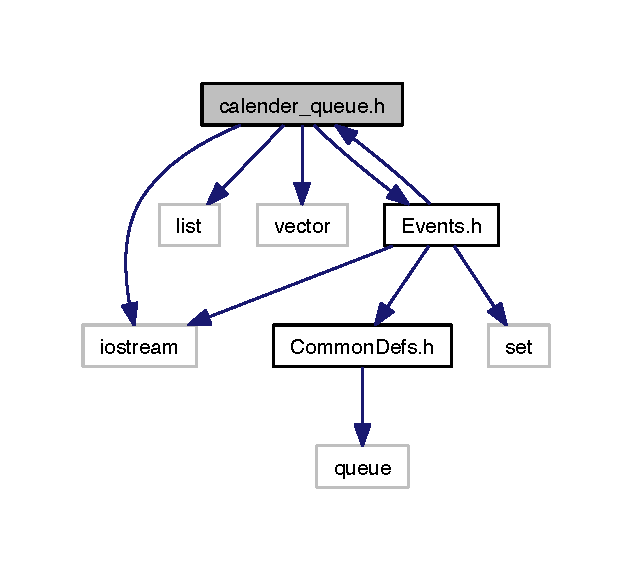
\includegraphics[width=303pt]{calender__queue_8h__incl}
\end{center}
\end{figure}
This graph shows which files directly or indirectly include this file\-:\nopagebreak
\begin{figure}[H]
\begin{center}
\leavevmode
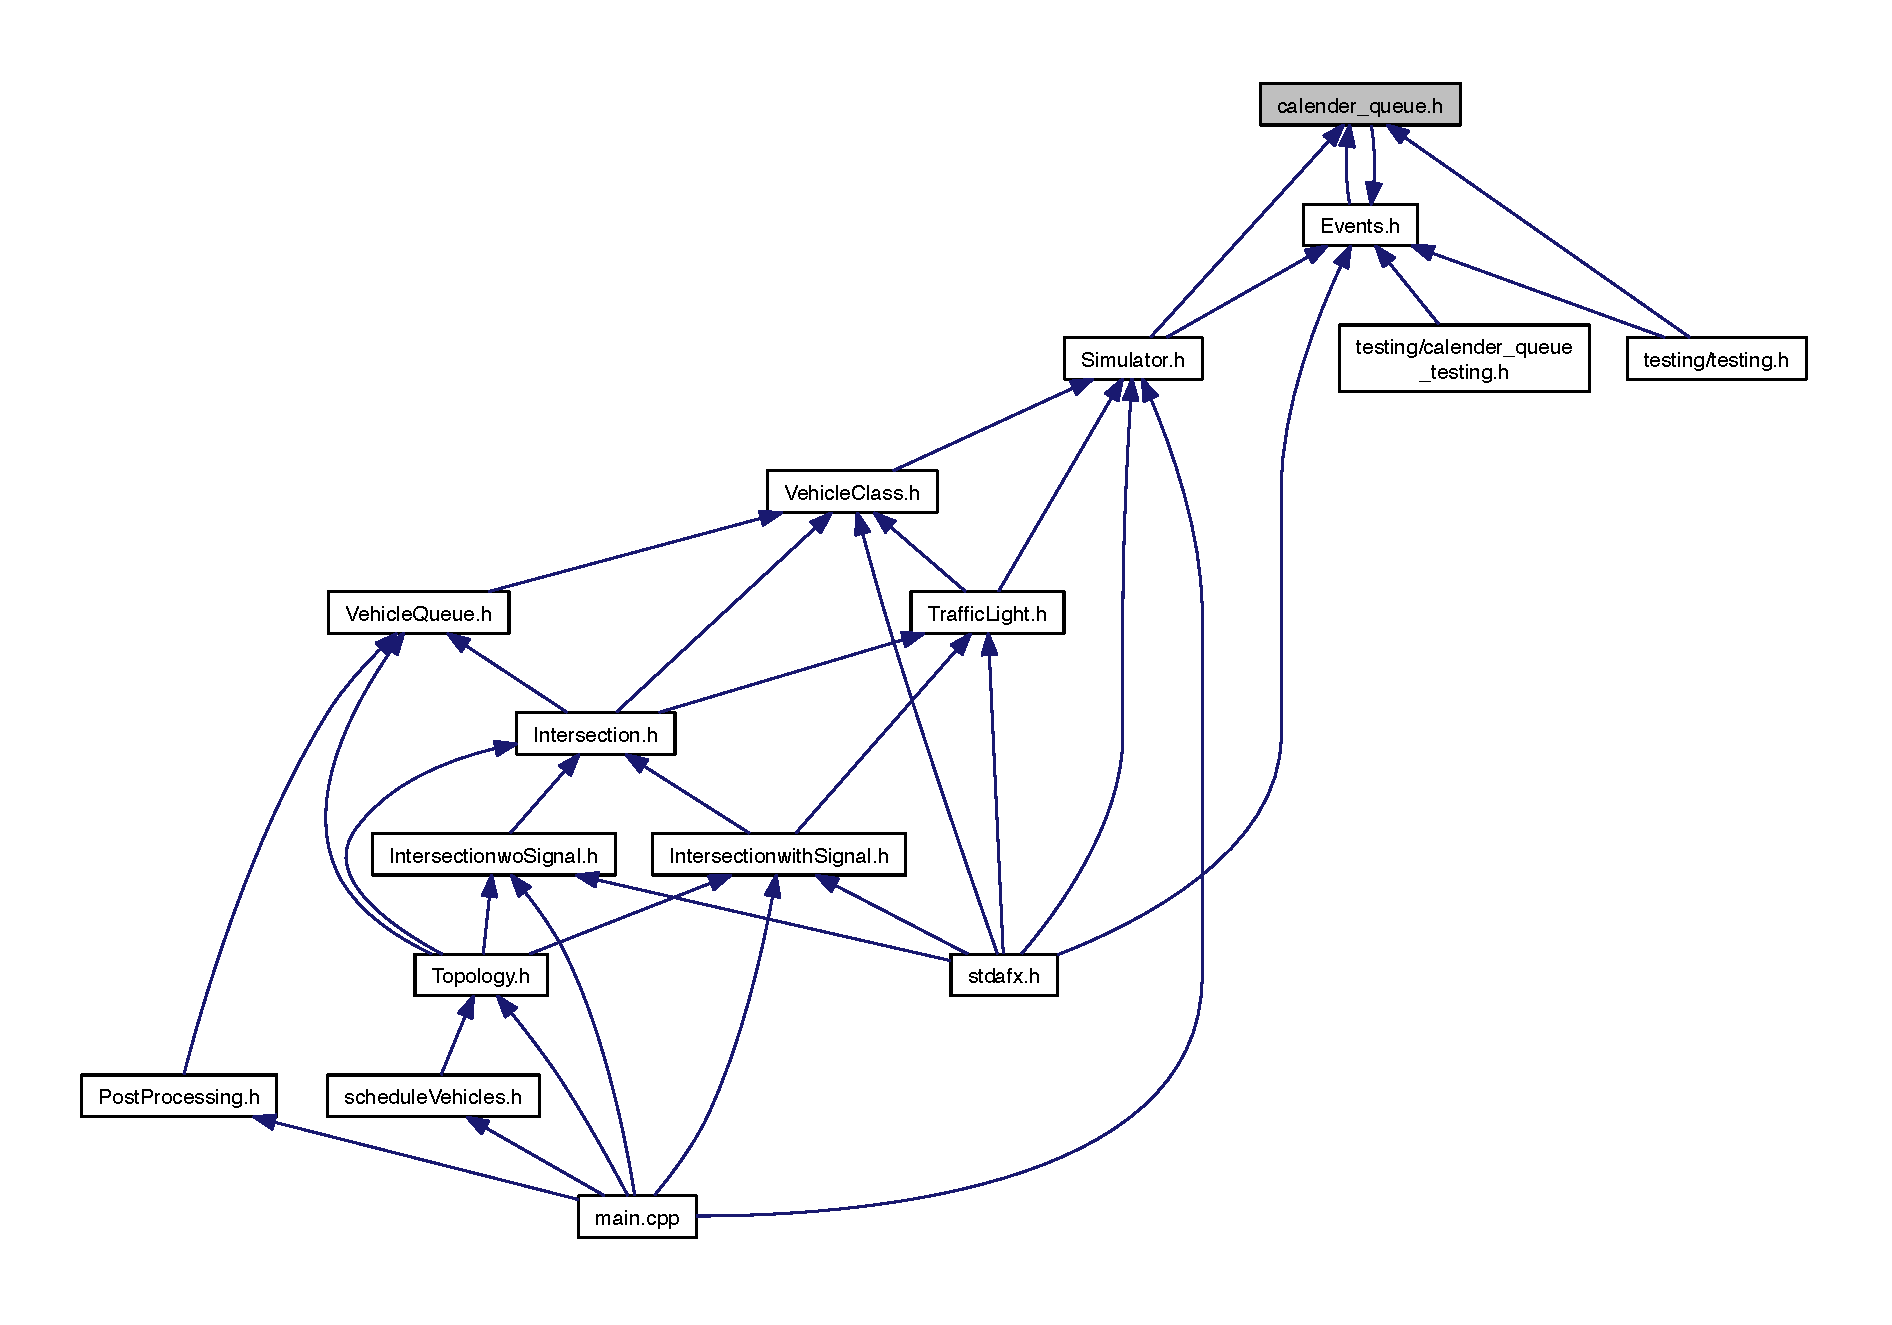
\includegraphics[width=350pt]{calender__queue_8h__dep__incl}
\end{center}
\end{figure}
\subsection*{Classes}
\begin{DoxyCompactItemize}
\item 
class \hyperlink{classcalender__queue}{calender\-\_\-queue}
\end{DoxyCompactItemize}
\subsection*{Macros}
\begin{DoxyCompactItemize}
\item 
\#define \hyperlink{calender__queue_8h_abd5c70d32425bb863d03547829782194}{T\-O\-T\-A\-L\-\_\-\-T\-I\-M\-E}~120$\ast$60
\item 
\#define \hyperlink{calender__queue_8h_a1072bf234f0898ff3c3b0c453c8adf45}{B\-U\-C\-K\-E\-T\-\_\-\-C\-O\-U\-N\-T}~72000
\item 
\hypertarget{calender__queue_8h_a352964ca100791f7e6438323f55b8541}{\#define {\bfseries B\-U\-C\-K\-E\-T\-\_\-\-S\-I\-Z\-E}~0.\-1}\label{calender__queue_8h_a352964ca100791f7e6438323f55b8541}

\item 
\#define \hyperlink{calender__queue_8h_a897e22608586c2928b305de5bd4e9bb8}{C\-A\-L\-E\-N\-D\-E\-R\-\_\-\-P\-E\-R\-I\-O\-D}~\hyperlink{calender__queue_8h_a1072bf234f0898ff3c3b0c453c8adf45}{B\-U\-C\-K\-E\-T\-\_\-\-C\-O\-U\-N\-T}$\ast$B\-U\-C\-K\-E\-T\-\_\-\-S\-I\-Z\-E
\end{DoxyCompactItemize}
\subsection*{Typedefs}
\begin{DoxyCompactItemize}
\item 
\hypertarget{calender__queue_8h_ab6530df477a1bf2804e6865497b288e3}{typedef std\-::list$<$ \hyperlink{class_event_base}{Event\-Base} $\ast$ $>$ {\bfseries bucket}}\label{calender__queue_8h_ab6530df477a1bf2804e6865497b288e3}

\end{DoxyCompactItemize}


\subsection{Detailed Description}
declartion of the class calender queue 

\subsection{Macro Definition Documentation}
\hypertarget{calender__queue_8h_a1072bf234f0898ff3c3b0c453c8adf45}{\index{calender\-\_\-queue.\-h@{calender\-\_\-queue.\-h}!B\-U\-C\-K\-E\-T\-\_\-\-C\-O\-U\-N\-T@{B\-U\-C\-K\-E\-T\-\_\-\-C\-O\-U\-N\-T}}
\index{B\-U\-C\-K\-E\-T\-\_\-\-C\-O\-U\-N\-T@{B\-U\-C\-K\-E\-T\-\_\-\-C\-O\-U\-N\-T}!calender_queue.h@{calender\-\_\-queue.\-h}}
\subsubsection[{B\-U\-C\-K\-E\-T\-\_\-\-C\-O\-U\-N\-T}]{\setlength{\rightskip}{0pt plus 5cm}\#define B\-U\-C\-K\-E\-T\-\_\-\-C\-O\-U\-N\-T~72000}}\label{calender__queue_8h_a1072bf234f0898ff3c3b0c453c8adf45}
Number of Buckets for Calender Queue \hypertarget{calender__queue_8h_a897e22608586c2928b305de5bd4e9bb8}{\index{calender\-\_\-queue.\-h@{calender\-\_\-queue.\-h}!C\-A\-L\-E\-N\-D\-E\-R\-\_\-\-P\-E\-R\-I\-O\-D@{C\-A\-L\-E\-N\-D\-E\-R\-\_\-\-P\-E\-R\-I\-O\-D}}
\index{C\-A\-L\-E\-N\-D\-E\-R\-\_\-\-P\-E\-R\-I\-O\-D@{C\-A\-L\-E\-N\-D\-E\-R\-\_\-\-P\-E\-R\-I\-O\-D}!calender_queue.h@{calender\-\_\-queue.\-h}}
\subsubsection[{C\-A\-L\-E\-N\-D\-E\-R\-\_\-\-P\-E\-R\-I\-O\-D}]{\setlength{\rightskip}{0pt plus 5cm}\#define C\-A\-L\-E\-N\-D\-E\-R\-\_\-\-P\-E\-R\-I\-O\-D~{\bf B\-U\-C\-K\-E\-T\-\_\-\-C\-O\-U\-N\-T}$\ast$B\-U\-C\-K\-E\-T\-\_\-\-S\-I\-Z\-E}}\label{calender__queue_8h_a897e22608586c2928b305de5bd4e9bb8}
how much is a \char`\"{}year\char`\"{} for this calender \hypertarget{calender__queue_8h_abd5c70d32425bb863d03547829782194}{\index{calender\-\_\-queue.\-h@{calender\-\_\-queue.\-h}!T\-O\-T\-A\-L\-\_\-\-T\-I\-M\-E@{T\-O\-T\-A\-L\-\_\-\-T\-I\-M\-E}}
\index{T\-O\-T\-A\-L\-\_\-\-T\-I\-M\-E@{T\-O\-T\-A\-L\-\_\-\-T\-I\-M\-E}!calender_queue.h@{calender\-\_\-queue.\-h}}
\subsubsection[{T\-O\-T\-A\-L\-\_\-\-T\-I\-M\-E}]{\setlength{\rightskip}{0pt plus 5cm}\#define T\-O\-T\-A\-L\-\_\-\-T\-I\-M\-E~120$\ast$60}}\label{calender__queue_8h_abd5c70d32425bb863d03547829782194}
Total time of the simulation 
\hypertarget{_common_defs_8h}{\section{Common\-Defs.\-h File Reference}
\label{_common_defs_8h}\index{Common\-Defs.\-h@{Common\-Defs.\-h}}
}
{\ttfamily \#include $<$queue$>$}\\*
Include dependency graph for Common\-Defs.\-h\-:\nopagebreak
\begin{figure}[H]
\begin{center}
\leavevmode
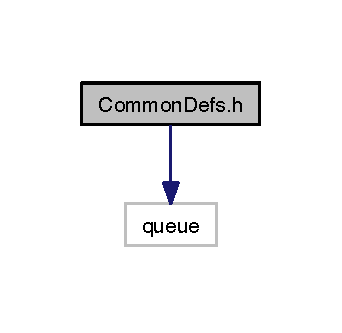
\includegraphics[width=164pt]{_common_defs_8h__incl}
\end{center}
\end{figure}
This graph shows which files directly or indirectly include this file\-:\nopagebreak
\begin{figure}[H]
\begin{center}
\leavevmode
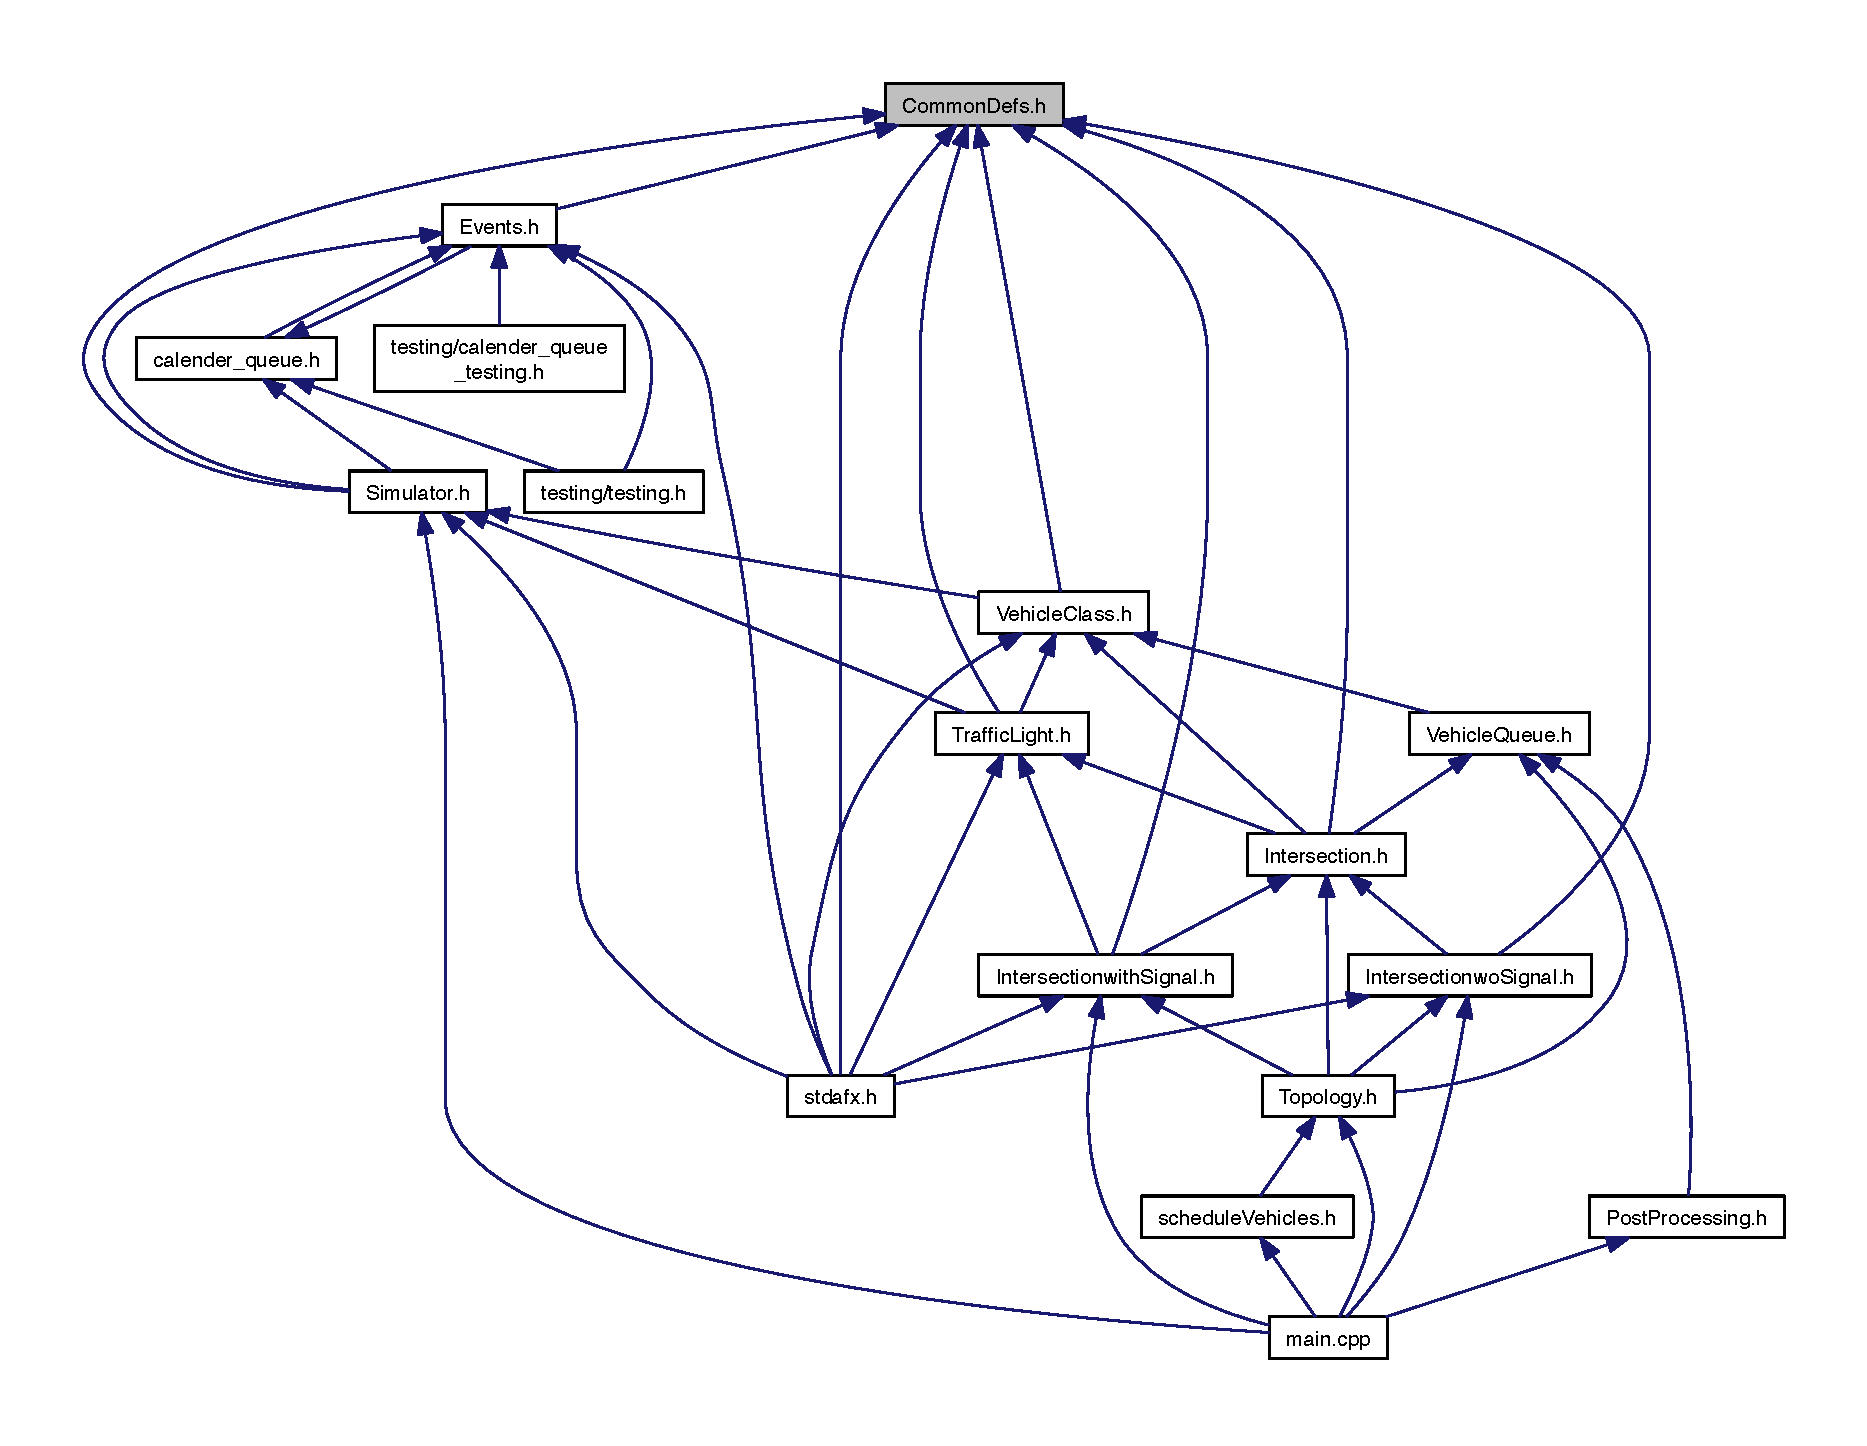
\includegraphics[width=350pt]{_common_defs_8h__dep__incl}
\end{center}
\end{figure}
\subsection*{Macros}
\begin{DoxyCompactItemize}
\item 
\hypertarget{_common_defs_8h_a5606b78ad32ff40800d9c4cbecfe72fd}{\#define {\bfseries \-\_\-\-\_\-\-C\-O\-M\-M\-O\-N\-\_\-\-D\-E\-F\-S\-\_\-\-H\-\_\-\-\_\-}}\label{_common_defs_8h_a5606b78ad32ff40800d9c4cbecfe72fd}

\item 
\#define \hyperlink{_common_defs_8h_aeb463ebe07f549555c0e4cbb049219fc}{Pass\-Time}~2.\-0
\item 
\#define \hyperlink{_common_defs_8h_ad25f5048846b180d445c3d4684a9c826}{start\-To\-Pass}~2.\-0
\item 
\#define \hyperlink{_common_defs_8h_aff59525ba6b86ffad48cb91df0152cc7}{L\-Pass\-Time}~3.\-0
\item 
\#define \hyperlink{_common_defs_8h_a4981ab751ab3a6f1f87f74d20909790f}{road\-Seg\-Time}~10.\-0
\item 
\#define \hyperlink{_common_defs_8h_accc6d973f7e650162ca12f2f4ff6420d}{check\-Qinterval}~2.\-0
\item 
\#define \hyperlink{_common_defs_8h_a203965ae780742a7d33284e735a3a481}{Burst\-Time}~2.\-0
\end{DoxyCompactItemize}
\subsection*{Typedefs}
\begin{DoxyCompactItemize}
\item 
typedef double \hyperlink{_common_defs_8h_a80b23eab88362163e2edd1a8b8238ef1}{Time\-\_\-t}
\end{DoxyCompactItemize}
\subsection*{Enumerations}
\begin{DoxyCompactItemize}
\item 
enum {\bfseries state} \{ \\*
{\bfseries G\-L\-T}, 
{\bfseries Y\-L\-T}, 
{\bfseries R\-L\-T}, 
{\bfseries G\-T\-R}, 
\\*
{\bfseries Y\-T\-R}, 
{\bfseries R\-T\-R}
 \}
\item 
enum {\bfseries dir} \{ {\bfseries N}, 
{\bfseries S}, 
{\bfseries E}, 
{\bfseries W}
 \}
\end{DoxyCompactItemize}
\subsection*{Functions}
\begin{DoxyCompactItemize}
\item 
int \hyperlink{_common_defs_8h_aee7862becfb6aef94f34e882348eb275}{reg} (int i)
\item 
int \hyperlink{_common_defs_8h_ab16114155cb6c7b1080dc8f52f1f8f7a}{turn} (dir global\-Dir, int Q\-Direction)
\end{DoxyCompactItemize}


\subsection{Detailed Description}
Contains commmon definations of various parameters used in different functions 

\subsection{Macro Definition Documentation}
\hypertarget{_common_defs_8h_a203965ae780742a7d33284e735a3a481}{\index{Common\-Defs.\-h@{Common\-Defs.\-h}!Burst\-Time@{Burst\-Time}}
\index{Burst\-Time@{Burst\-Time}!CommonDefs.h@{Common\-Defs.\-h}}
\subsubsection[{Burst\-Time}]{\setlength{\rightskip}{0pt plus 5cm}\#define Burst\-Time~2.\-0}}\label{_common_defs_8h_a203965ae780742a7d33284e735a3a481}
time for the next vehicle to depart when cars are going in groups \hypertarget{_common_defs_8h_accc6d973f7e650162ca12f2f4ff6420d}{\index{Common\-Defs.\-h@{Common\-Defs.\-h}!check\-Qinterval@{check\-Qinterval}}
\index{check\-Qinterval@{check\-Qinterval}!CommonDefs.h@{Common\-Defs.\-h}}
\subsubsection[{check\-Qinterval}]{\setlength{\rightskip}{0pt plus 5cm}\#define check\-Qinterval~2.\-0}}\label{_common_defs_8h_accc6d973f7e650162ca12f2f4ff6420d}
if the next Q is full, check again in this amout of time \hypertarget{_common_defs_8h_aff59525ba6b86ffad48cb91df0152cc7}{\index{Common\-Defs.\-h@{Common\-Defs.\-h}!L\-Pass\-Time@{L\-Pass\-Time}}
\index{L\-Pass\-Time@{L\-Pass\-Time}!CommonDefs.h@{Common\-Defs.\-h}}
\subsubsection[{L\-Pass\-Time}]{\setlength{\rightskip}{0pt plus 5cm}\#define L\-Pass\-Time~3.\-0}}\label{_common_defs_8h_aff59525ba6b86ffad48cb91df0152cc7}
service time to turn left in seconds (debug) \hypertarget{_common_defs_8h_aeb463ebe07f549555c0e4cbb049219fc}{\index{Common\-Defs.\-h@{Common\-Defs.\-h}!Pass\-Time@{Pass\-Time}}
\index{Pass\-Time@{Pass\-Time}!CommonDefs.h@{Common\-Defs.\-h}}
\subsubsection[{Pass\-Time}]{\setlength{\rightskip}{0pt plus 5cm}\#define Pass\-Time~2.\-0}}\label{_common_defs_8h_aeb463ebe07f549555c0e4cbb049219fc}
service time to go straight in seconds \hypertarget{_common_defs_8h_a4981ab751ab3a6f1f87f74d20909790f}{\index{Common\-Defs.\-h@{Common\-Defs.\-h}!road\-Seg\-Time@{road\-Seg\-Time}}
\index{road\-Seg\-Time@{road\-Seg\-Time}!CommonDefs.h@{Common\-Defs.\-h}}
\subsubsection[{road\-Seg\-Time}]{\setlength{\rightskip}{0pt plus 5cm}\#define road\-Seg\-Time~10.\-0}}\label{_common_defs_8h_a4981ab751ab3a6f1f87f74d20909790f}
time to travel one road segment \hypertarget{_common_defs_8h_ad25f5048846b180d445c3d4684a9c826}{\index{Common\-Defs.\-h@{Common\-Defs.\-h}!start\-To\-Pass@{start\-To\-Pass}}
\index{start\-To\-Pass@{start\-To\-Pass}!CommonDefs.h@{Common\-Defs.\-h}}
\subsubsection[{start\-To\-Pass}]{\setlength{\rightskip}{0pt plus 5cm}\#define start\-To\-Pass~2.\-0}}\label{_common_defs_8h_ad25f5048846b180d445c3d4684a9c826}
when a queue is empty and a vehicle arrives, it takes this much to depart 

\subsection{Typedef Documentation}
\hypertarget{_common_defs_8h_a80b23eab88362163e2edd1a8b8238ef1}{\index{Common\-Defs.\-h@{Common\-Defs.\-h}!Time\-\_\-t@{Time\-\_\-t}}
\index{Time\-\_\-t@{Time\-\_\-t}!CommonDefs.h@{Common\-Defs.\-h}}
\subsubsection[{Time\-\_\-t}]{\setlength{\rightskip}{0pt plus 5cm}typedef double {\bf Time\-\_\-t}}}\label{_common_defs_8h_a80b23eab88362163e2edd1a8b8238ef1}
Type for storing simulation times 

\subsection{Function Documentation}
\hypertarget{_common_defs_8h_aee7862becfb6aef94f34e882348eb275}{\index{Common\-Defs.\-h@{Common\-Defs.\-h}!reg@{reg}}
\index{reg@{reg}!CommonDefs.h@{Common\-Defs.\-h}}
\subsubsection[{reg}]{\setlength{\rightskip}{0pt plus 5cm}int reg (
\begin{DoxyParamCaption}
\item[{int}]{i}
\end{DoxyParamCaption}
)}}\label{_common_defs_8h_aee7862becfb6aef94f34e882348eb275}
\begin{DoxySeeAlso}{See Also}
intersection.\-cpp 
\end{DoxySeeAlso}


Here is the call graph for this function\-:\nopagebreak
\begin{figure}[H]
\begin{center}
\leavevmode
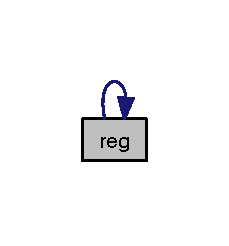
\includegraphics[width=110pt]{_common_defs_8h_aee7862becfb6aef94f34e882348eb275_cgraph}
\end{center}
\end{figure}


\hypertarget{_common_defs_8h_ab16114155cb6c7b1080dc8f52f1f8f7a}{\index{Common\-Defs.\-h@{Common\-Defs.\-h}!turn@{turn}}
\index{turn@{turn}!CommonDefs.h@{Common\-Defs.\-h}}
\subsubsection[{turn}]{\setlength{\rightskip}{0pt plus 5cm}int turn (
\begin{DoxyParamCaption}
\item[{dir}]{global\-Dir, }
\item[{int}]{Q\-Direction}
\end{DoxyParamCaption}
)}}\label{_common_defs_8h_ab16114155cb6c7b1080dc8f52f1f8f7a}
Returns routing address for Vehicle \begin{DoxySeeAlso}{See Also}
intersection.\-cpp 
\end{DoxySeeAlso}


Here is the call graph for this function\-:\nopagebreak
\begin{figure}[H]
\begin{center}
\leavevmode
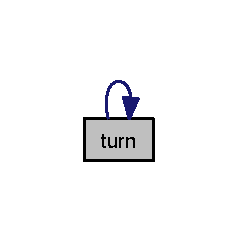
\includegraphics[width=114pt]{_common_defs_8h_ab16114155cb6c7b1080dc8f52f1f8f7a_cgraph}
\end{center}
\end{figure}



\hypertarget{_events_8h}{\section{Events.\-h File Reference}
\label{_events_8h}\index{Events.\-h@{Events.\-h}}
}


declaration of various types of events  


{\ttfamily \#include \char`\"{}Common\-Defs.\-h\char`\"{}}\\*
{\ttfamily \#include $<$set$>$}\\*
{\ttfamily \#include $<$iostream$>$}\\*
{\ttfamily \#include \char`\"{}calender\-\_\-queue.\-h\char`\"{}}\\*
Include dependency graph for Events.\-h\-:\nopagebreak
\begin{figure}[H]
\begin{center}
\leavevmode
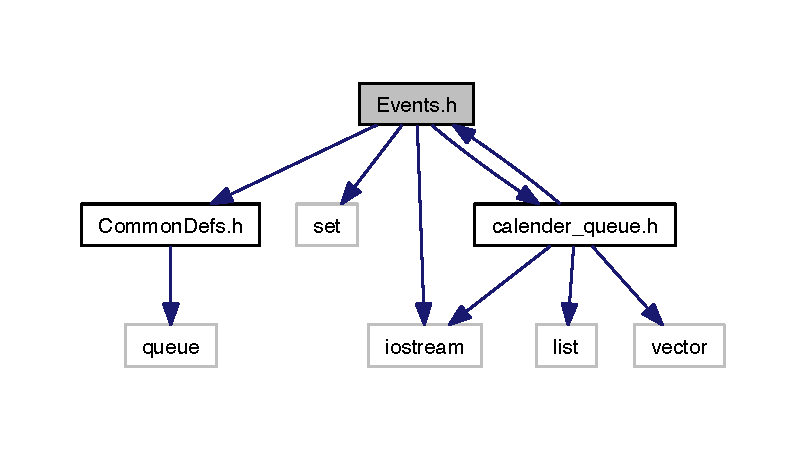
\includegraphics[width=350pt]{_events_8h__incl}
\end{center}
\end{figure}
This graph shows which files directly or indirectly include this file\-:
\nopagebreak
\begin{figure}[H]
\begin{center}
\leavevmode
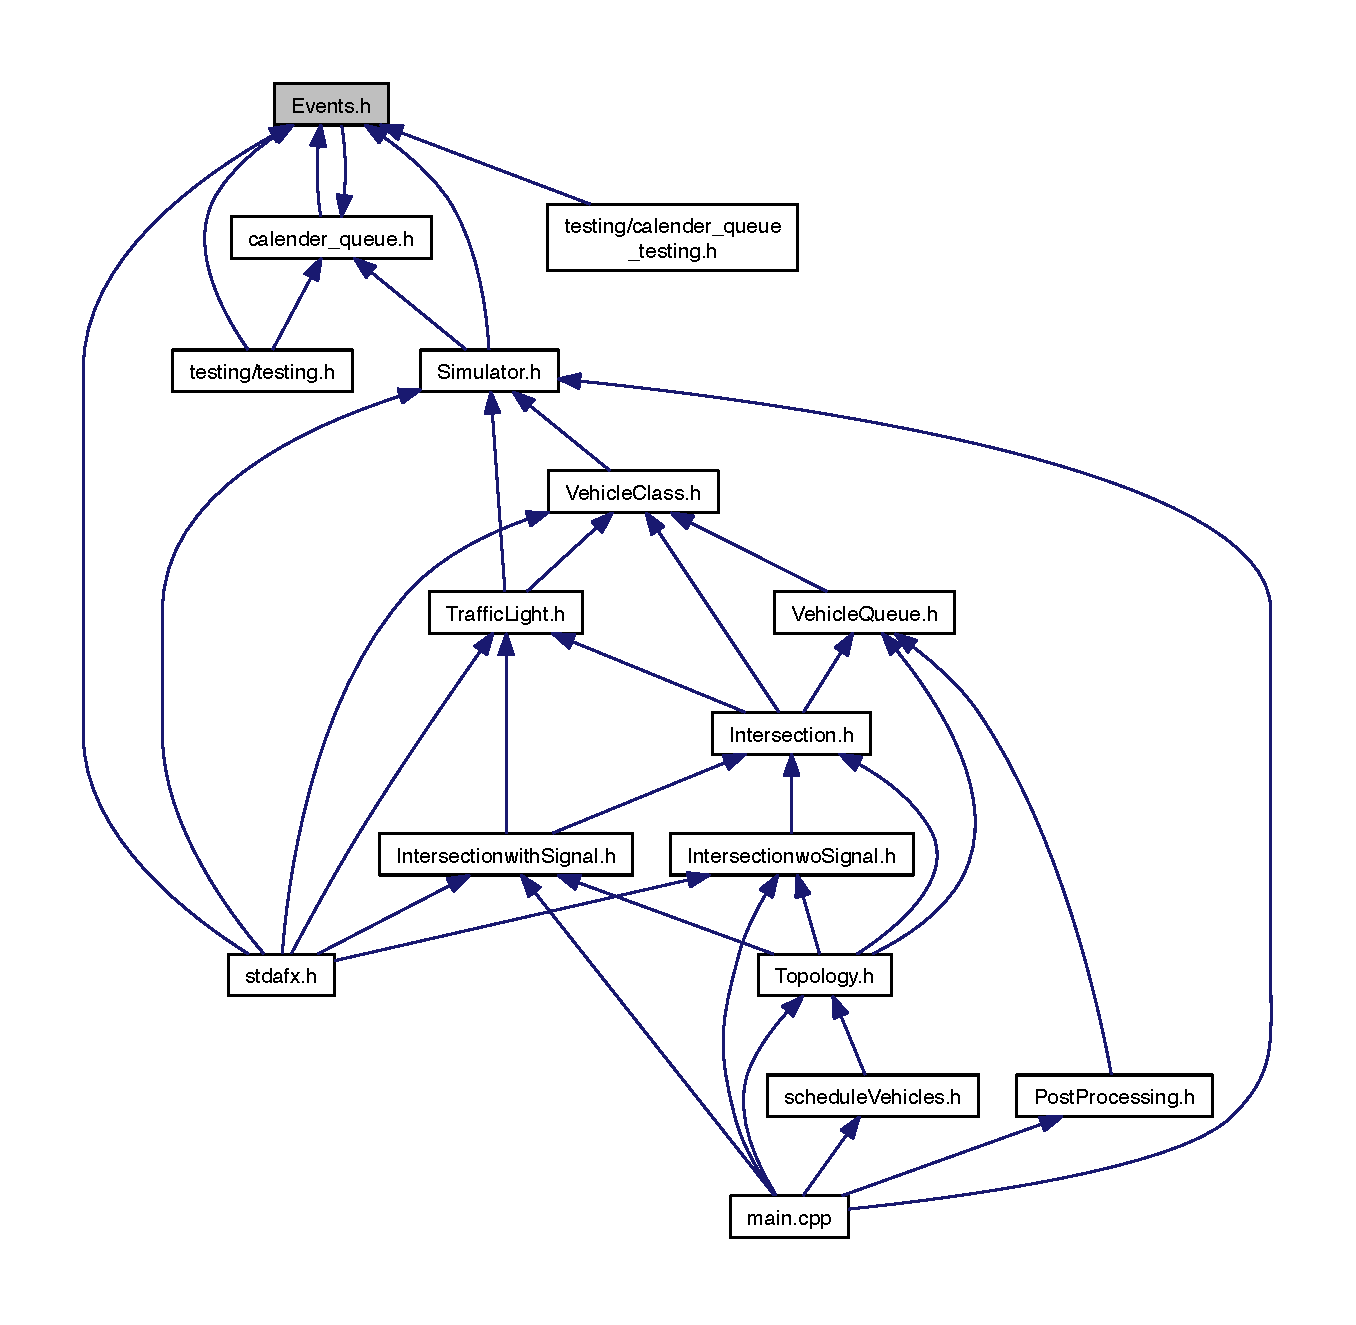
\includegraphics[width=350pt]{_events_8h__dep__incl}
\end{center}
\end{figure}
\subsection*{Classes}
\begin{DoxyCompactItemize}
\item 
class \hyperlink{class_event_base}{Event\-Base}
\item 
class \hyperlink{class_event0}{Event0$<$ T, O\-B\-J $>$}
\item 
class \hyperlink{class_event1}{Event1$<$ T, O\-B\-J, U1, T1 $>$}
\item 
class \hyperlink{class_event2}{Event2$<$ T, O\-B\-J, U1, T1, U2, T2 $>$}
\item 
class \hyperlink{class_event3}{Event3$<$ T, O\-B\-J, U1, T1, U2, T2, U3, T3 $>$}
\item 
class \hyperlink{classevent__compare}{event\-\_\-compare}
\end{DoxyCompactItemize}


\subsection{Detailed Description}
declaration of various types of events 
\hypertarget{_intersection_8h}{\section{Intersection.\-h File Reference}
\label{_intersection_8h}\index{Intersection.\-h@{Intersection.\-h}}
}
{\ttfamily \#include $<$queue$>$}\\*
{\ttfamily \#include \char`\"{}Common\-Defs.\-h\char`\"{}}\\*
{\ttfamily \#include \char`\"{}Traffic\-Light.\-h\char`\"{}}\\*
{\ttfamily \#include \char`\"{}Vehicle\-Class.\-h\char`\"{}}\\*
{\ttfamily \#include \char`\"{}Vehicle\-Queue.\-h\char`\"{}}\\*
Include dependency graph for Intersection.\-h\-:\nopagebreak
\begin{figure}[H]
\begin{center}
\leavevmode
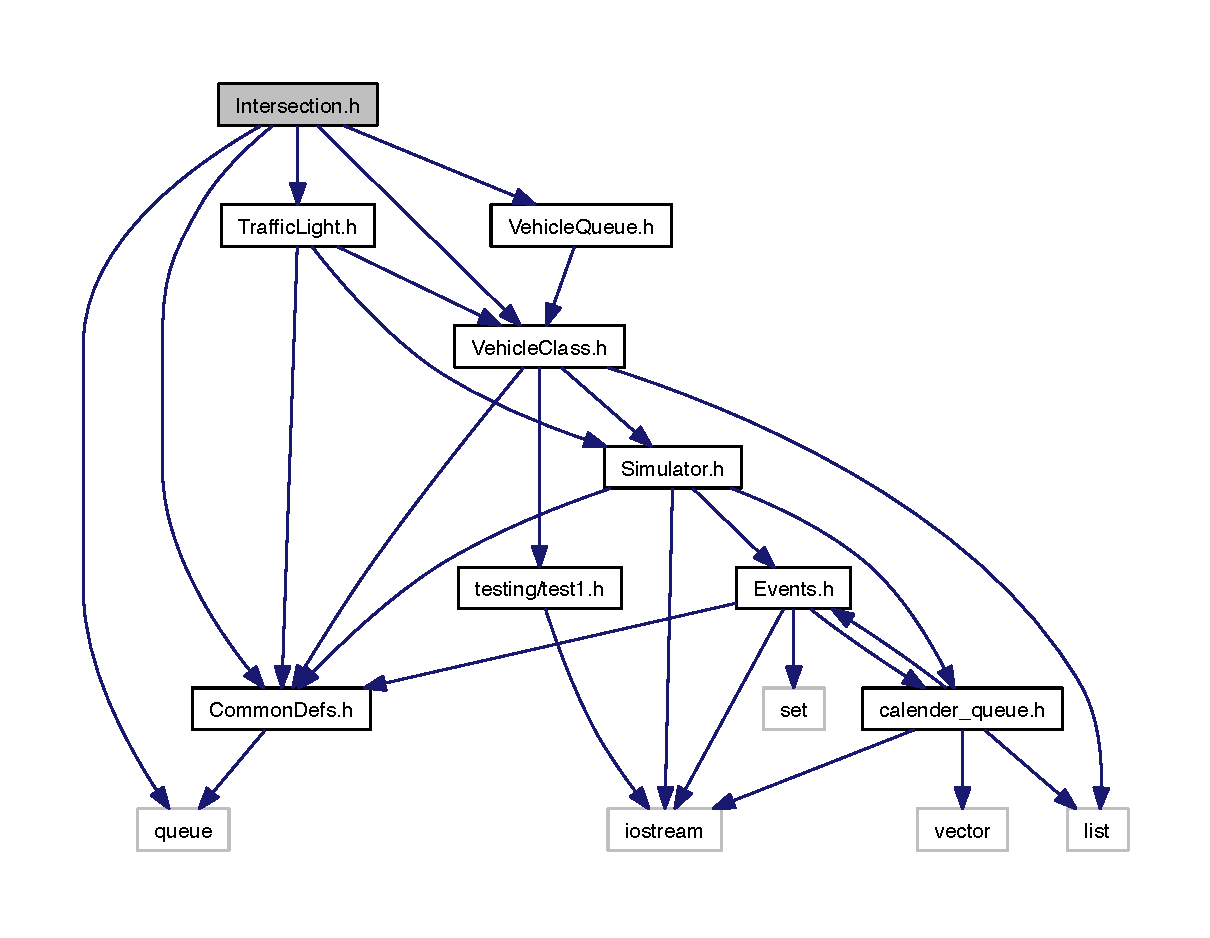
\includegraphics[width=350pt]{_intersection_8h__incl}
\end{center}
\end{figure}
This graph shows which files directly or indirectly include this file\-:\nopagebreak
\begin{figure}[H]
\begin{center}
\leavevmode
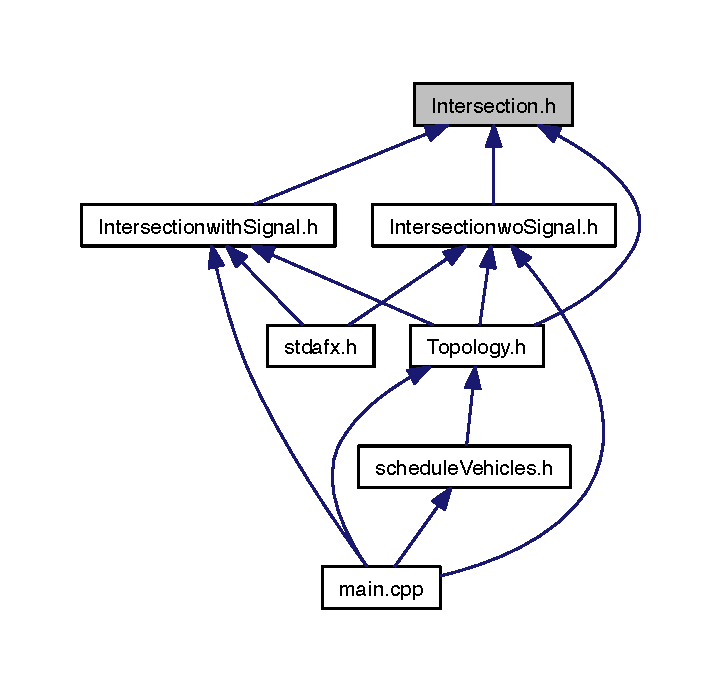
\includegraphics[width=347pt]{_intersection_8h__dep__incl}
\end{center}
\end{figure}
\subsection*{Classes}
\begin{DoxyCompactItemize}
\item 
class \hyperlink{class_intersection}{Intersection}
\end{DoxyCompactItemize}


\subsection{Detailed Description}
Contains base class intersection from which both intersectionwithsignal and intersectionwosignal inherit \begin{DoxySeeAlso}{See Also}
\hyperlink{_intersectionwith_signal_8h}{Intersectionwith\-Signal.\-h} 

\hyperlink{_intersectionwo_signal_8h}{Intersectionwo\-Signal.\-h} 
\end{DoxySeeAlso}

\hypertarget{_intersectionwith_signal_8h}{\section{Intersectionwith\-Signal.\-h File Reference}
\label{_intersectionwith_signal_8h}\index{Intersectionwith\-Signal.\-h@{Intersectionwith\-Signal.\-h}}
}
{\ttfamily \#include $<$queue$>$}\\*
{\ttfamily \#include \char`\"{}Common\-Defs.\-h\char`\"{}}\\*
{\ttfamily \#include \char`\"{}Traffic\-Light.\-h\char`\"{}}\\*
{\ttfamily \#include \char`\"{}Intersection.\-h\char`\"{}}\\*
Include dependency graph for Intersectionwith\-Signal.\-h\-:\nopagebreak
\begin{figure}[H]
\begin{center}
\leavevmode
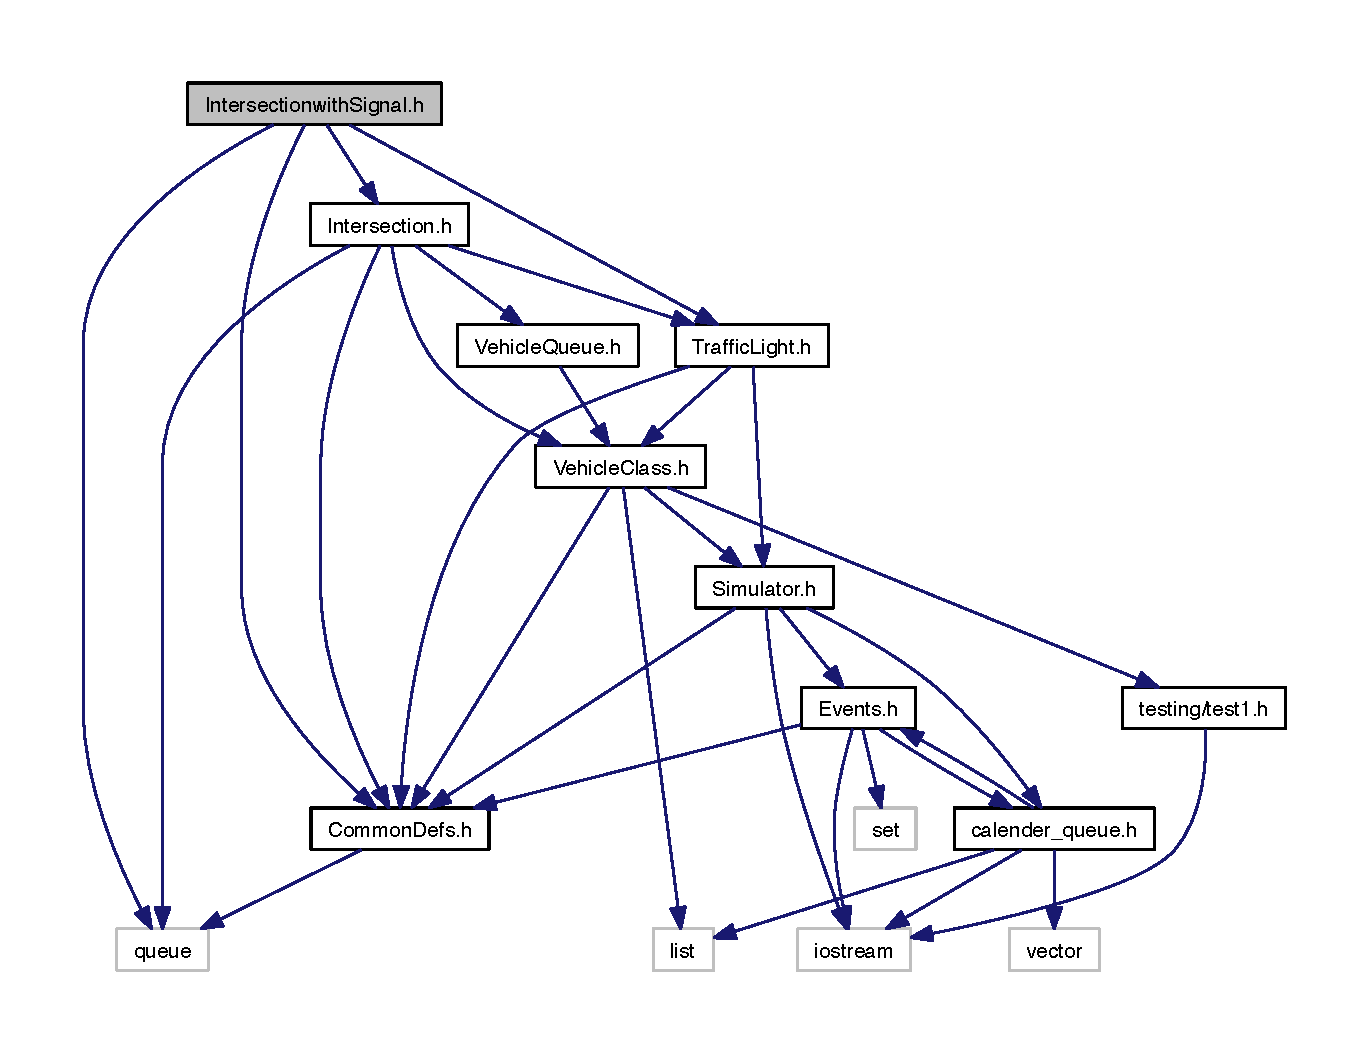
\includegraphics[width=350pt]{_intersectionwith_signal_8h__incl}
\end{center}
\end{figure}
This graph shows which files directly or indirectly include this file\-:\nopagebreak
\begin{figure}[H]
\begin{center}
\leavevmode
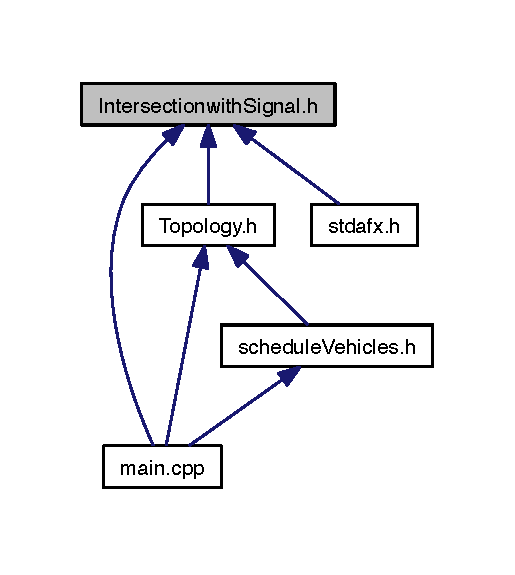
\includegraphics[width=247pt]{_intersectionwith_signal_8h__dep__incl}
\end{center}
\end{figure}
\subsection*{Classes}
\begin{DoxyCompactItemize}
\item 
class \hyperlink{class_intersectionwith_signal}{Intersectionwith\-Signal}
\end{DoxyCompactItemize}


\subsection{Detailed Description}
Description of \hyperlink{class_intersection}{Intersection} with traffic signals class \begin{DoxySeeAlso}{See Also}
\hyperlink{_intersection_8h}{Intersection.\-h} 
\end{DoxySeeAlso}

\hypertarget{_intersectionwo_signal_8h}{\section{Intersectionwo\-Signal.\-h File Reference}
\label{_intersectionwo_signal_8h}\index{Intersectionwo\-Signal.\-h@{Intersectionwo\-Signal.\-h}}
}
{\ttfamily \#include $<$queue$>$}\\*
{\ttfamily \#include \char`\"{}Common\-Defs.\-h\char`\"{}}\\*
{\ttfamily \#include \char`\"{}Intersection.\-h\char`\"{}}\\*
Include dependency graph for Intersectionwo\-Signal.\-h\-:\nopagebreak
\begin{figure}[H]
\begin{center}
\leavevmode
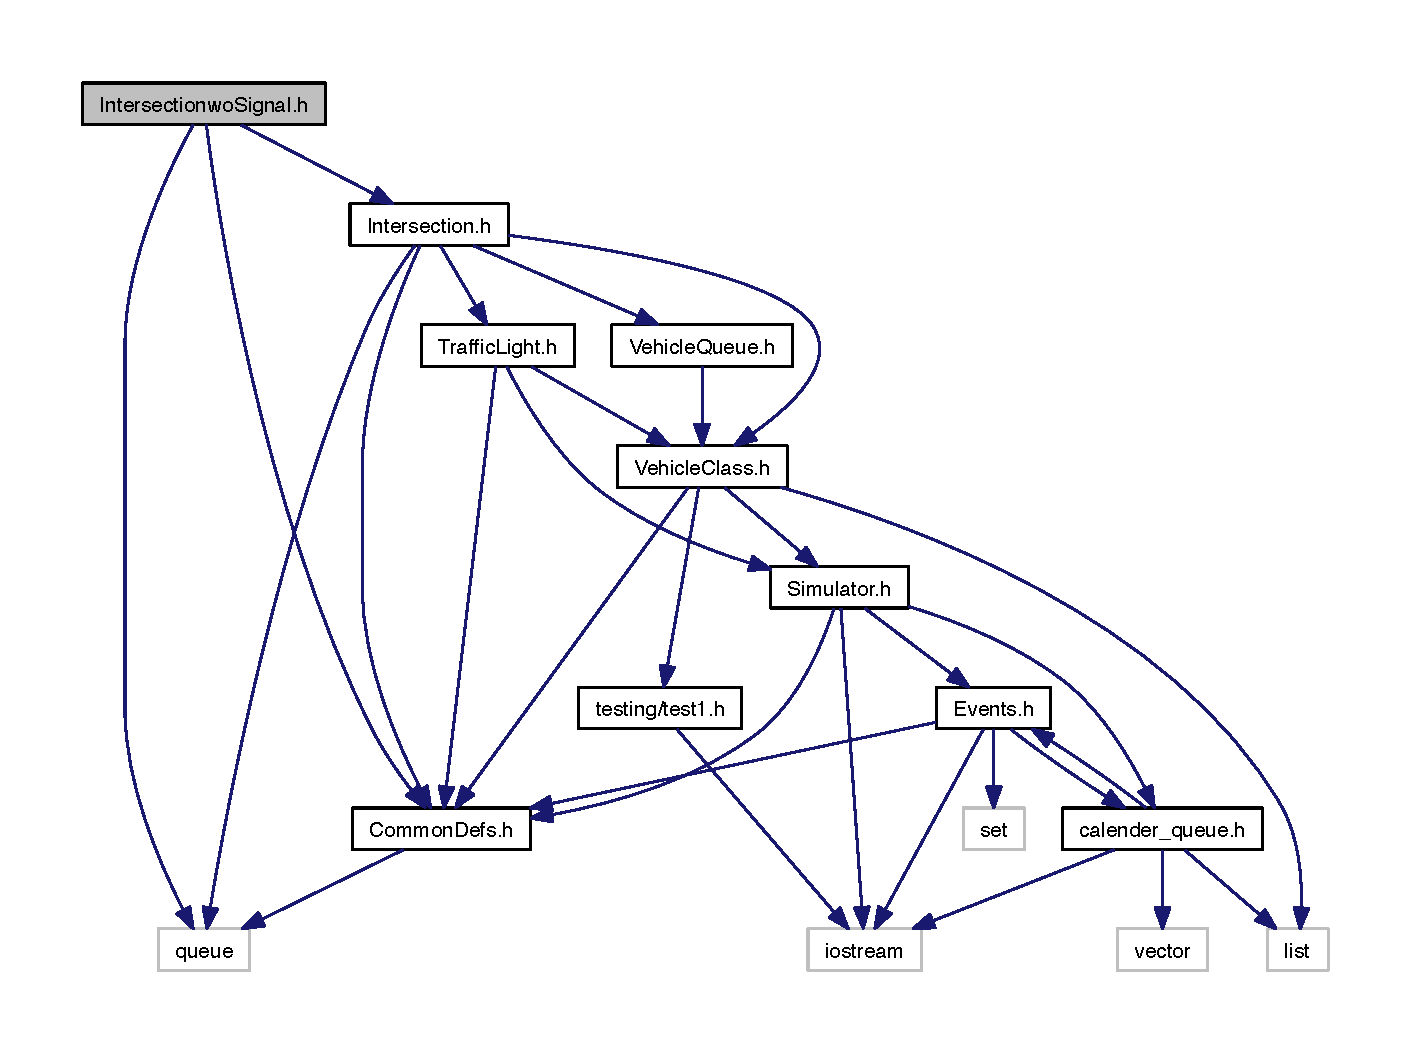
\includegraphics[width=350pt]{_intersectionwo_signal_8h__incl}
\end{center}
\end{figure}
This graph shows which files directly or indirectly include this file\-:\nopagebreak
\begin{figure}[H]
\begin{center}
\leavevmode
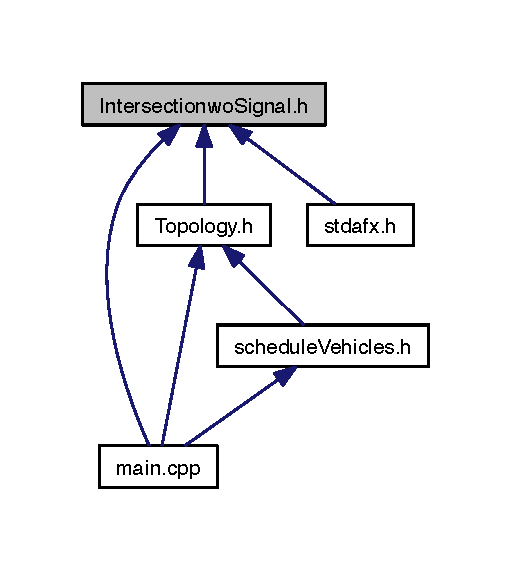
\includegraphics[width=245pt]{_intersectionwo_signal_8h__dep__incl}
\end{center}
\end{figure}
\subsection*{Classes}
\begin{DoxyCompactItemize}
\item 
class \hyperlink{class_intersectionwithout_signal}{Intersectionwithout\-Signal}
\end{DoxyCompactItemize}


\subsection{Detailed Description}
Description of \hyperlink{class_intersection}{Intersection} with out traffic signals class \begin{DoxySeeAlso}{See Also}
\hyperlink{_intersection_8h}{Intersection.\-h} 
\end{DoxySeeAlso}

\hypertarget{main_8cpp}{\section{main.\-cpp File Reference}
\label{main_8cpp}\index{main.\-cpp@{main.\-cpp}}
}
{\ttfamily \#include $<$iostream$>$}\\*
{\ttfamily \#include $<$fstream$>$}\\*
{\ttfamily \#include \char`\"{}Simulator.\-h\char`\"{}}\\*
{\ttfamily \#include \char`\"{}Intersectionwith\-Signal.\-h\char`\"{}}\\*
{\ttfamily \#include \char`\"{}Intersectionwo\-Signal.\-h\char`\"{}}\\*
{\ttfamily \#include \char`\"{}Topology.\-h\char`\"{}}\\*
{\ttfamily \#include \char`\"{}schedule\-Vehicles.\-h\char`\"{}}\\*
{\ttfamily \#include \char`\"{}Post\-Processing.\-h\char`\"{}}\\*
{\ttfamily \#include \char`\"{}testing/test1.\-h\char`\"{}}\\*
{\ttfamily \#include $<$queue$>$}\\*
Include dependency graph for main.\-cpp\-:\nopagebreak
\begin{figure}[H]
\begin{center}
\leavevmode
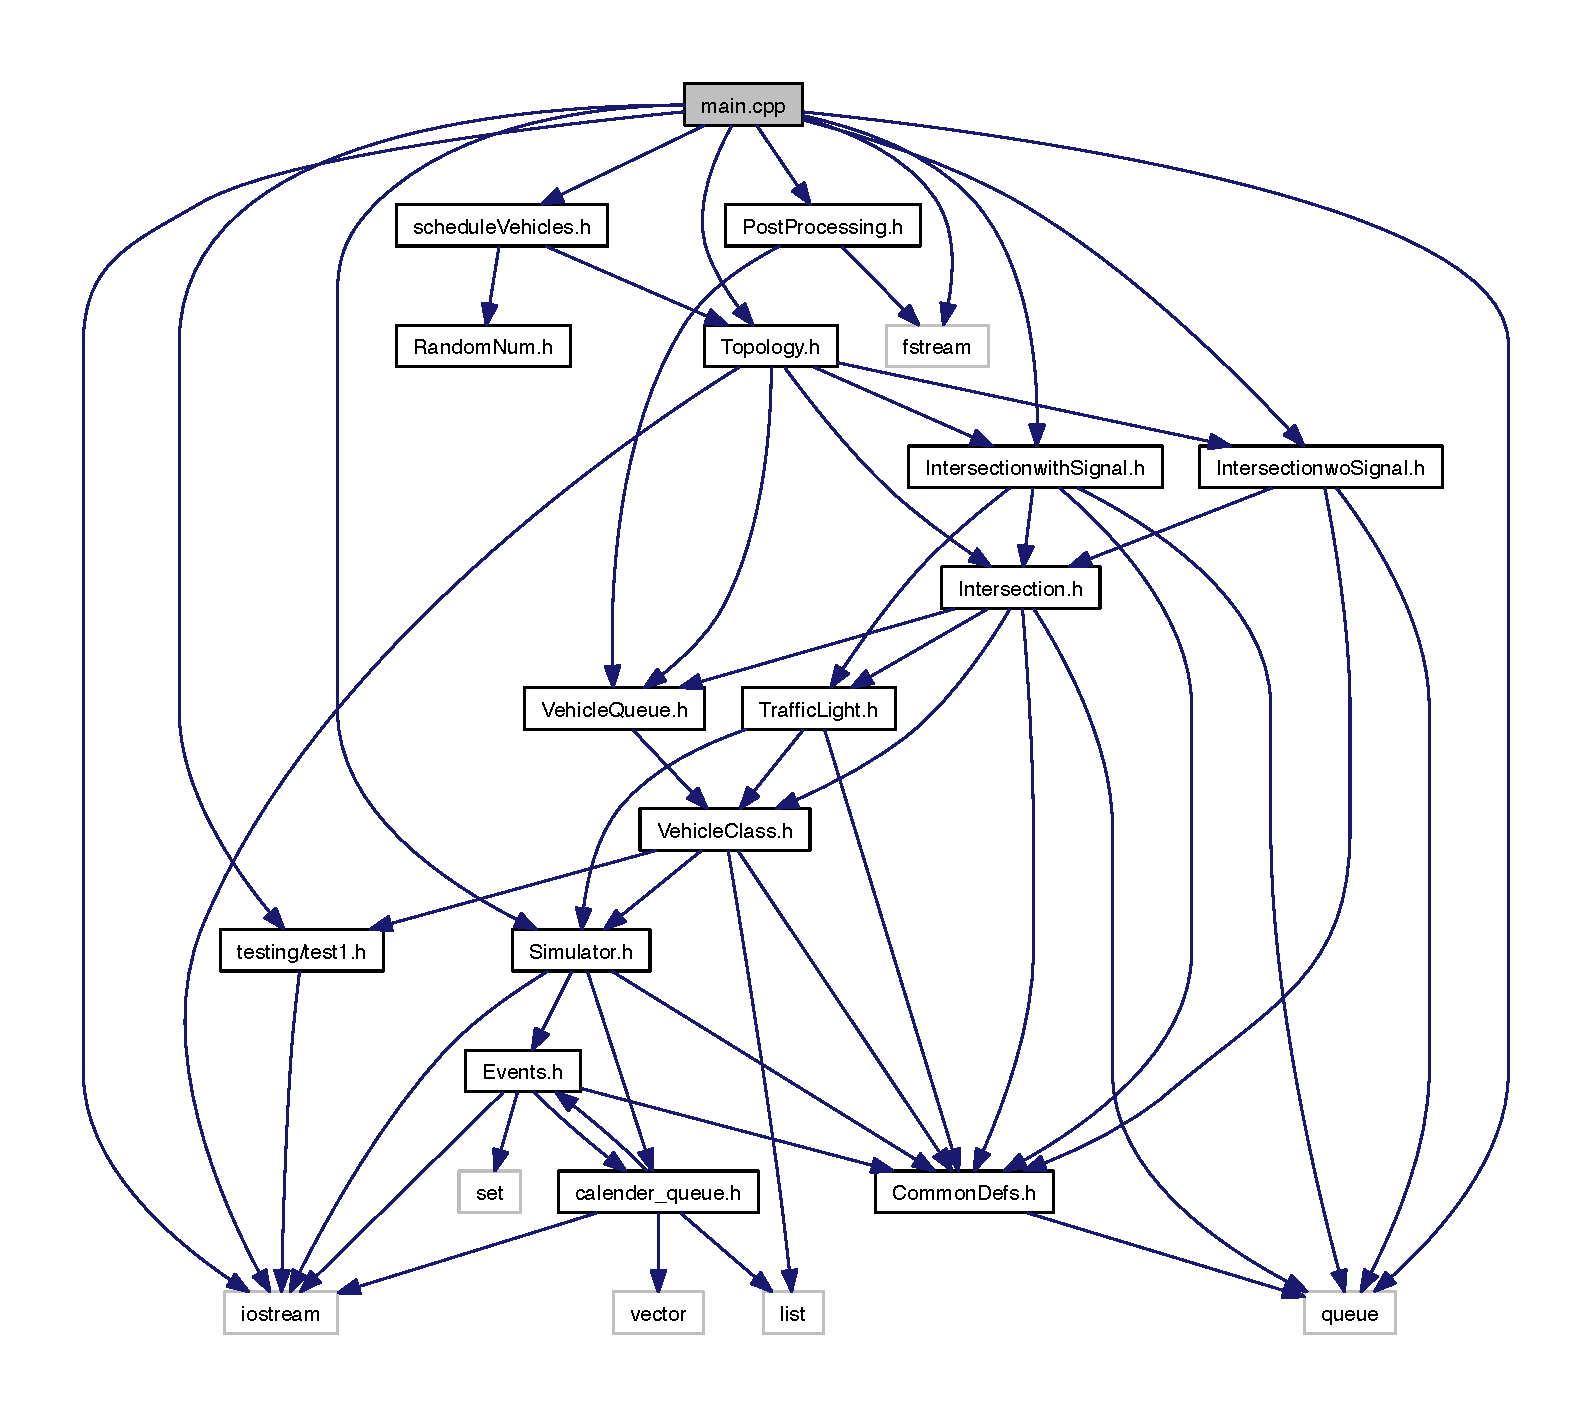
\includegraphics[width=350pt]{main_8cpp__incl}
\end{center}
\end{figure}
\subsection*{Functions}
\begin{DoxyCompactItemize}
\item 
\hypertarget{main_8cpp_ae66f6b31b5ad750f1fe042a706a4e3d4}{int {\bfseries main} ()}\label{main_8cpp_ae66f6b31b5ad750f1fe042a706a4e3d4}

\end{DoxyCompactItemize}
\subsection*{Variables}
\begin{DoxyCompactItemize}
\item 
\hypertarget{main_8cpp_a8ffc0a8a399f474857b353e5d8997e05}{\hyperlink{class_simulator}{Simulator} $\ast$ {\bfseries sim} = new \hyperlink{class_simulator}{Simulator}()}\label{main_8cpp_a8ffc0a8a399f474857b353e5d8997e05}

\end{DoxyCompactItemize}

\hypertarget{_post_processing_8h}{\section{Post\-Processing.\-h File Reference}
\label{_post_processing_8h}\index{Post\-Processing.\-h@{Post\-Processing.\-h}}
}
{\ttfamily \#include $<$fstream$>$}\\*
{\ttfamily \#include \char`\"{}Vehicle\-Queue.\-h\char`\"{}}\\*
Include dependency graph for Post\-Processing.\-h\-:\nopagebreak
\begin{figure}[H]
\begin{center}
\leavevmode
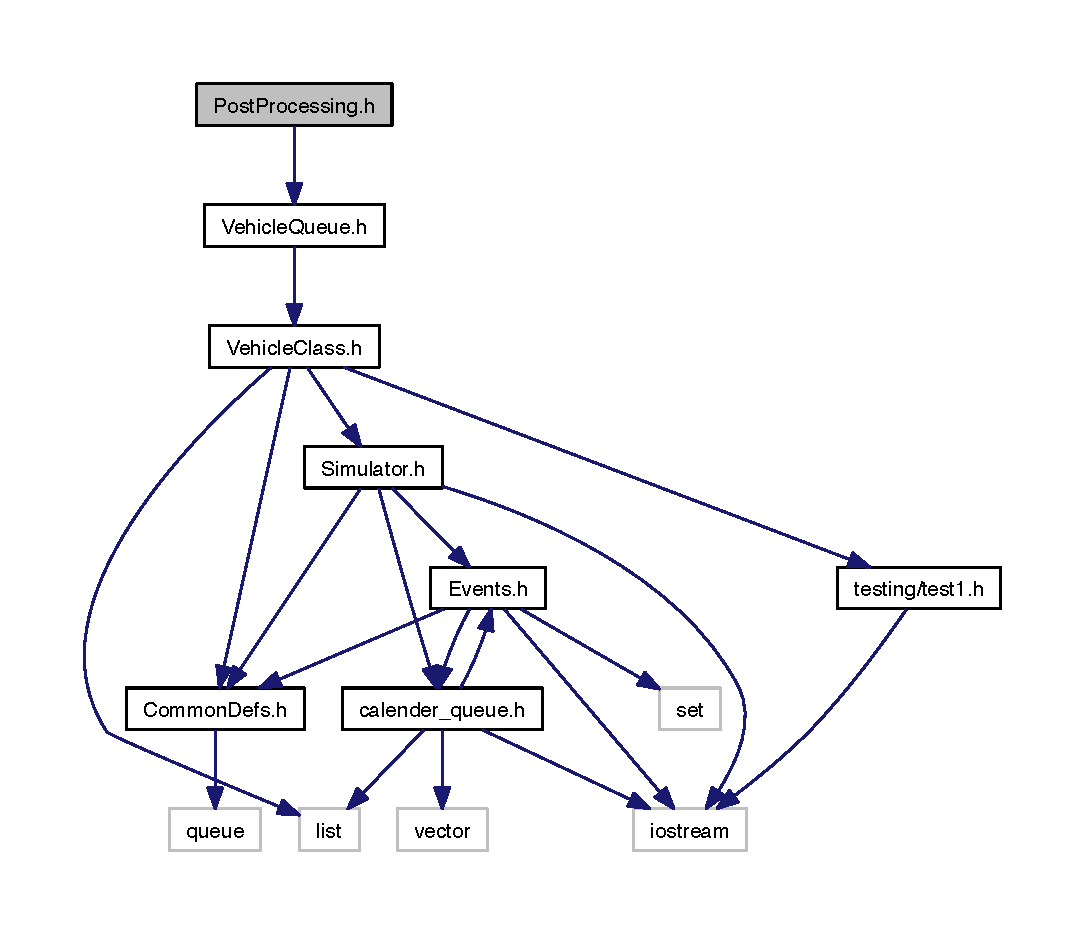
\includegraphics[width=350pt]{_post_processing_8h__incl}
\end{center}
\end{figure}
This graph shows which files directly or indirectly include this file\-:\nopagebreak
\begin{figure}[H]
\begin{center}
\leavevmode
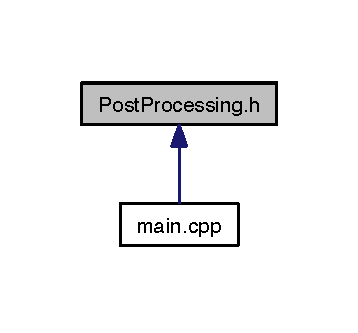
\includegraphics[width=172pt]{_post_processing_8h__dep__incl}
\end{center}
\end{figure}
\subsection*{Functions}
\begin{DoxyCompactItemize}
\item 
void \hyperlink{_post_processing_8h_a55d4f3188204db01a47e44eb6d99a70a}{Post\-Proc\-Stats} (\hyperlink{class_vehicle_queue}{Vehicle\-Queue} $\ast$Ex\-Q, double timeval, int buckets, int source, int dest, ofstream \&fh)
\end{DoxyCompactItemize}


\subsection{Detailed Description}
Takes Exit Queue As Argument and print Various following things
\begin{DoxyEnumerate}
\item Histogram of simulation time 
\end{DoxyEnumerate}

\subsection{Function Documentation}
\hypertarget{_post_processing_8h_a55d4f3188204db01a47e44eb6d99a70a}{\index{Post\-Processing.\-h@{Post\-Processing.\-h}!Post\-Proc\-Stats@{Post\-Proc\-Stats}}
\index{Post\-Proc\-Stats@{Post\-Proc\-Stats}!PostProcessing.h@{Post\-Processing.\-h}}
\subsubsection[{Post\-Proc\-Stats}]{\setlength{\rightskip}{0pt plus 5cm}void Post\-Proc\-Stats (
\begin{DoxyParamCaption}
\item[{{\bf Vehicle\-Queue} $\ast$}]{Ex\-Q, }
\item[{double}]{timeval, }
\item[{int}]{buckets, }
\item[{int}]{source, }
\item[{int}]{dest, }
\item[{ofstream \&}]{fh}
\end{DoxyParamCaption}
)}}\label{_post_processing_8h_a55d4f3188204db01a47e44eb6d99a70a}
Takes exit queue and prints histogram of time takes to cover between source and destination Also prints stats like, average time , standard deviation etc. 
\begin{DoxyParams}{Parameters}
{\em E\-Q} & is exit Q \\
\hline
{\em buckets} & is number of buckets for histogram \\
\hline
{\em timeval} & is the period of time which is divided into buckets \\
\hline
{\em source} & is starting point of the journey \\
\hline
{\em dest} & is input for describing \\
\hline
\end{DoxyParams}


Here is the call graph for this function\-:\nopagebreak
\begin{figure}[H]
\begin{center}
\leavevmode
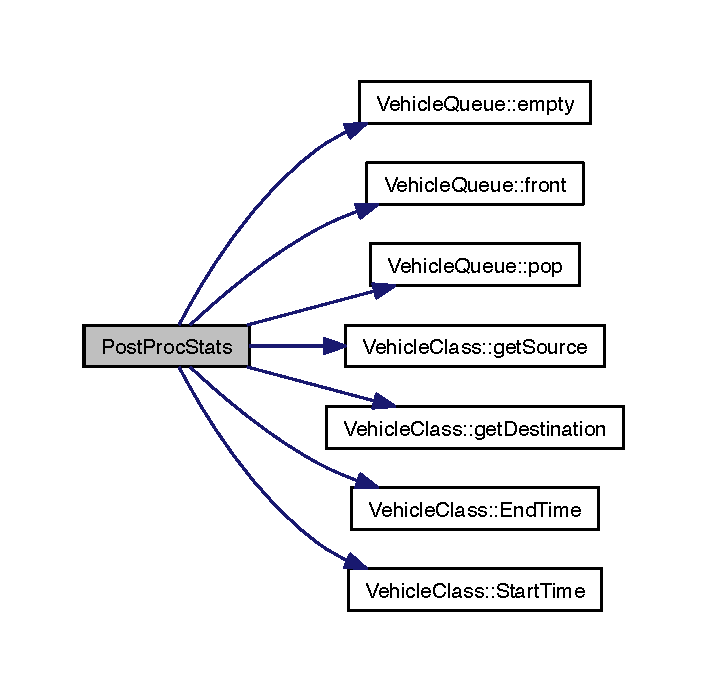
\includegraphics[width=340pt]{_post_processing_8h_a55d4f3188204db01a47e44eb6d99a70a_cgraph}
\end{center}
\end{figure}



\hypertarget{_random_num_8h}{\section{Random\-Num.\-h File Reference}
\label{_random_num_8h}\index{Random\-Num.\-h@{Random\-Num.\-h}}
}
This graph shows which files directly or indirectly include this file\-:
\nopagebreak
\begin{figure}[H]
\begin{center}
\leavevmode
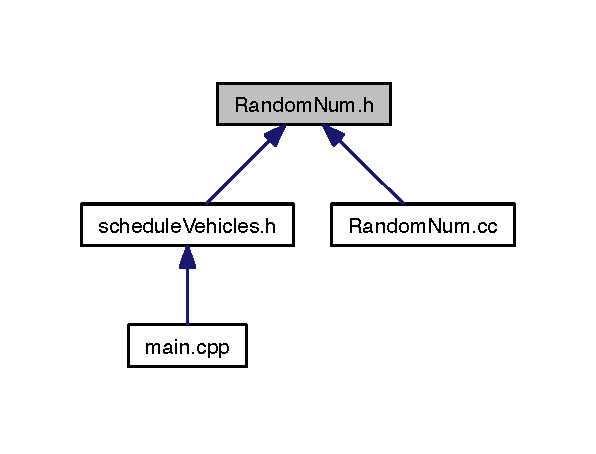
\includegraphics[width=286pt]{_random_num_8h__dep__incl}
\end{center}
\end{figure}
\subsection*{Classes}
\begin{DoxyCompactItemize}
\item 
class \hyperlink{class_random_num_gen}{Random\-Num\-Gen}
\end{DoxyCompactItemize}
\subsection*{Macros}
\begin{DoxyCompactItemize}
\item 
\#define \hyperlink{_random_num_8h_a10c053ba5cc085484425f965c90c8468}{M\-I\-N\-S\-T\-D\-X}~1
\item 
\#define \hyperlink{_random_num_8h_a06e731a88cba6df46e425e4424d692e2}{M\-I\-N\-S\-T\-D\-M}~2147483647
\item 
\#define \hyperlink{_random_num_8h_a11d6041d9eb53dc6a26b8c41dbaaba2d}{M\-I\-N\-S\-T\-D\-G}~16807
\end{DoxyCompactItemize}
\subsection*{Functions}
\begin{DoxyCompactItemize}
\item 
unsigned long \hyperlink{_random_num_8h_ad5a693f25861204ddea76b1ac59710bd}{gettime} ()
\end{DoxyCompactItemize}


\subsection{Detailed Description}
A Random number generator class. This class describes the implementation number genrator 

\subsection{Macro Definition Documentation}
\hypertarget{_random_num_8h_a11d6041d9eb53dc6a26b8c41dbaaba2d}{\index{Random\-Num.\-h@{Random\-Num.\-h}!M\-I\-N\-S\-T\-D\-G@{M\-I\-N\-S\-T\-D\-G}}
\index{M\-I\-N\-S\-T\-D\-G@{M\-I\-N\-S\-T\-D\-G}!RandomNum.h@{Random\-Num.\-h}}
\subsubsection[{M\-I\-N\-S\-T\-D\-G}]{\setlength{\rightskip}{0pt plus 5cm}\#define M\-I\-N\-S\-T\-D\-G~16807}}\label{_random_num_8h_a11d6041d9eb53dc6a26b8c41dbaaba2d}
Multiplier for random number genrator \hypertarget{_random_num_8h_a06e731a88cba6df46e425e4424d692e2}{\index{Random\-Num.\-h@{Random\-Num.\-h}!M\-I\-N\-S\-T\-D\-M@{M\-I\-N\-S\-T\-D\-M}}
\index{M\-I\-N\-S\-T\-D\-M@{M\-I\-N\-S\-T\-D\-M}!RandomNum.h@{Random\-Num.\-h}}
\subsubsection[{M\-I\-N\-S\-T\-D\-M}]{\setlength{\rightskip}{0pt plus 5cm}\#define M\-I\-N\-S\-T\-D\-M~2147483647}}\label{_random_num_8h_a06e731a88cba6df46e425e4424d692e2}
Modulus for random number genrator \hypertarget{_random_num_8h_a10c053ba5cc085484425f965c90c8468}{\index{Random\-Num.\-h@{Random\-Num.\-h}!M\-I\-N\-S\-T\-D\-X@{M\-I\-N\-S\-T\-D\-X}}
\index{M\-I\-N\-S\-T\-D\-X@{M\-I\-N\-S\-T\-D\-X}!RandomNum.h@{Random\-Num.\-h}}
\subsubsection[{M\-I\-N\-S\-T\-D\-X}]{\setlength{\rightskip}{0pt plus 5cm}\#define M\-I\-N\-S\-T\-D\-X~1}}\label{_random_num_8h_a10c053ba5cc085484425f965c90c8468}
Default starting state 

\subsection{Function Documentation}
\hypertarget{_random_num_8h_ad5a693f25861204ddea76b1ac59710bd}{\index{Random\-Num.\-h@{Random\-Num.\-h}!gettime@{gettime}}
\index{gettime@{gettime}!RandomNum.h@{Random\-Num.\-h}}
\subsubsection[{gettime}]{\setlength{\rightskip}{0pt plus 5cm}unsigned long gettime (
\begin{DoxyParamCaption}
\item[{void}]{}
\end{DoxyParamCaption}
)}}\label{_random_num_8h_ad5a693f25861204ddea76b1ac59710bd}
Time function to measure time 
\hypertarget{_road_segment_8h}{\section{Road\-Segment.\-h File Reference}
\label{_road_segment_8h}\index{Road\-Segment.\-h@{Road\-Segment.\-h}}
}
\subsection*{Classes}
\begin{DoxyCompactItemize}
\item 
class \hyperlink{class_road_segment}{Road\-Segment}
\end{DoxyCompactItemize}


\subsection{Detailed Description}
Define a segment of the Road 
\hypertarget{schedule_vehicles_8h}{\section{schedule\-Vehicles.\-h File Reference}
\label{schedule_vehicles_8h}\index{schedule\-Vehicles.\-h@{schedule\-Vehicles.\-h}}
}
{\ttfamily \#include \char`\"{}Topology.\-h\char`\"{}}\\*
{\ttfamily \#include \char`\"{}Random\-Num.\-h\char`\"{}}\\*
Include dependency graph for schedule\-Vehicles.\-h\-:\nopagebreak
\begin{figure}[H]
\begin{center}
\leavevmode
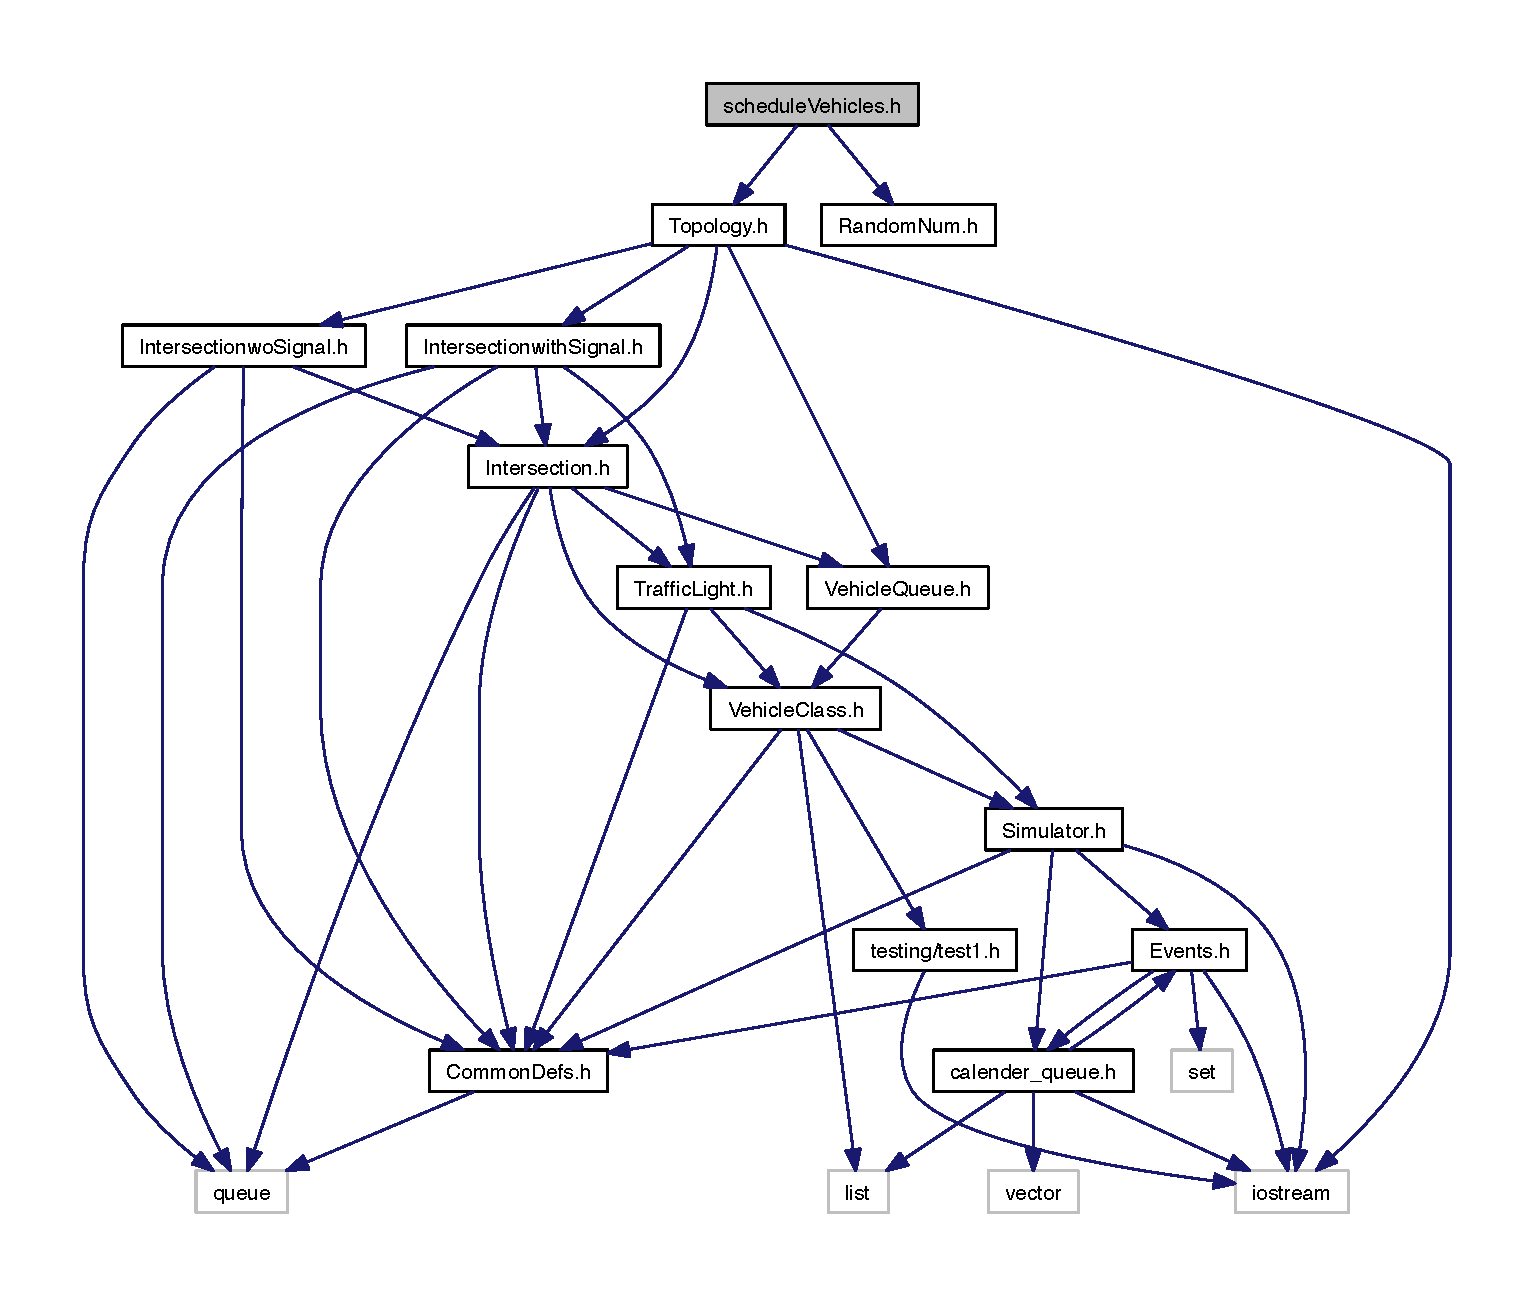
\includegraphics[width=350pt]{schedule_vehicles_8h__incl}
\end{center}
\end{figure}
This graph shows which files directly or indirectly include this file\-:\nopagebreak
\begin{figure}[H]
\begin{center}
\leavevmode
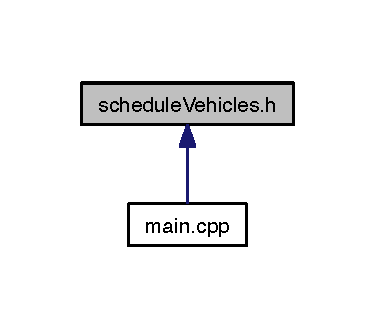
\includegraphics[width=180pt]{schedule_vehicles_8h__dep__incl}
\end{center}
\end{figure}
\subsection*{Functions}
\begin{DoxyCompactItemize}
\item 
void \hyperlink{schedule_vehicles_8h_a6fddfc87662e222a887bd35b5ba69518}{schedule\-Vehicles} (\hyperlink{class___topology}{\-\_\-\-Topology} $\ast$Topology, double max\-Time)
\end{DoxyCompactItemize}


\subsection{Detailed Description}
It initializes the scheduling of vehicle during the simulation 

\subsection{Function Documentation}
\hypertarget{schedule_vehicles_8h_a6fddfc87662e222a887bd35b5ba69518}{\index{schedule\-Vehicles.\-h@{schedule\-Vehicles.\-h}!schedule\-Vehicles@{schedule\-Vehicles}}
\index{schedule\-Vehicles@{schedule\-Vehicles}!scheduleVehicles.h@{schedule\-Vehicles.\-h}}
\subsubsection[{schedule\-Vehicles}]{\setlength{\rightskip}{0pt plus 5cm}void schedule\-Vehicles (
\begin{DoxyParamCaption}
\item[{{\bf \-\_\-\-Topology} $\ast$}]{Topology, }
\item[{double}]{max\-Time}
\end{DoxyParamCaption}
)}}\label{schedule_vehicles_8h_a6fddfc87662e222a887bd35b5ba69518}
It initializes the scheduling of vehicle during the simulation 
\begin{DoxyParams}{Parameters}
{\em Topology} & of the westpeachtree street \\
\hline
{\em max\-Time,maximum} & time of till which we have to schedule vehicles \\
\hline
\end{DoxyParams}


Here is the call graph for this function\-:
\nopagebreak
\begin{figure}[H]
\begin{center}
\leavevmode
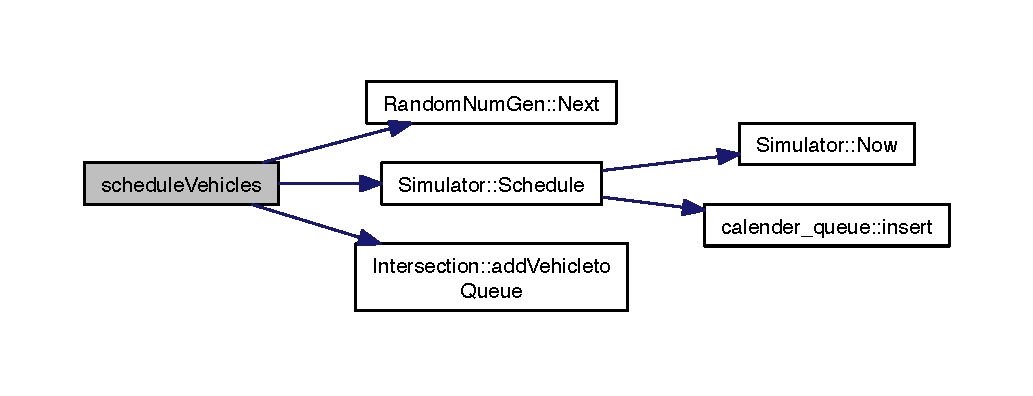
\includegraphics[width=350pt]{schedule_vehicles_8h_a6fddfc87662e222a887bd35b5ba69518_cgraph}
\end{center}
\end{figure}



\hypertarget{_simulator_8h}{\section{Simulator.\-h File Reference}
\label{_simulator_8h}\index{Simulator.\-h@{Simulator.\-h}}
}
{\ttfamily \#include $<$iostream$>$}\\*
{\ttfamily \#include \char`\"{}Common\-Defs.\-h\char`\"{}}\\*
{\ttfamily \#include \char`\"{}Events.\-h\char`\"{}}\\*
{\ttfamily \#include \char`\"{}calender\-\_\-queue.\-h\char`\"{}}\\*
Include dependency graph for Simulator.\-h\-:\nopagebreak
\begin{figure}[H]
\begin{center}
\leavevmode
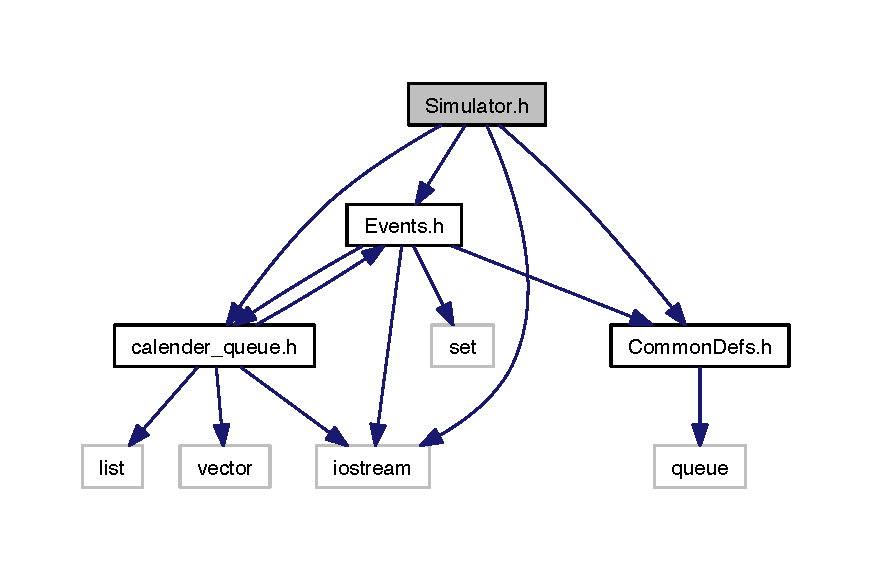
\includegraphics[width=350pt]{_simulator_8h__incl}
\end{center}
\end{figure}
This graph shows which files directly or indirectly include this file\-:\nopagebreak
\begin{figure}[H]
\begin{center}
\leavevmode
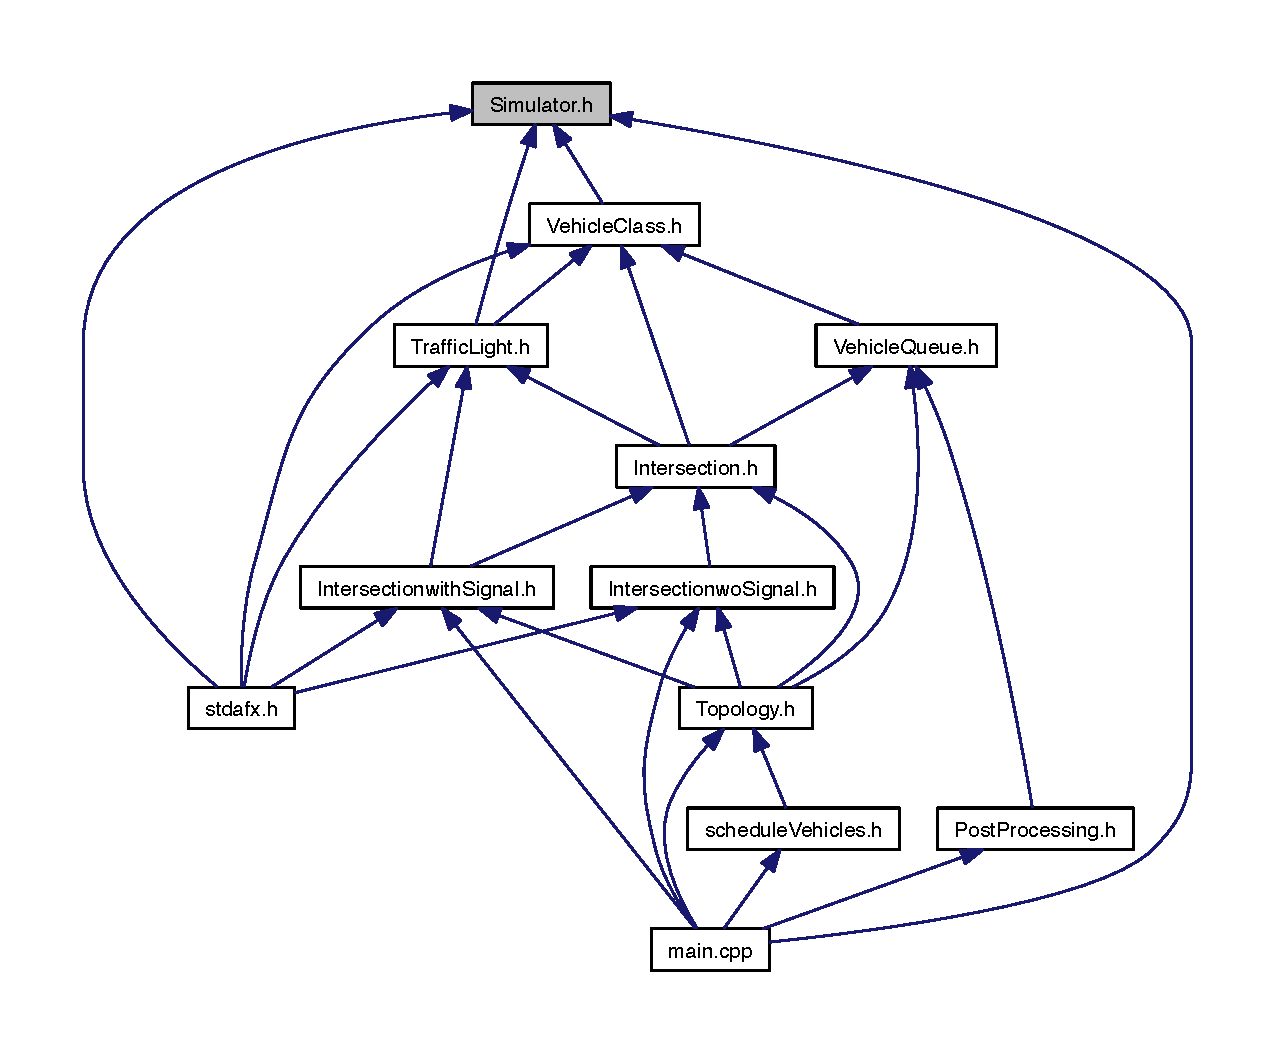
\includegraphics[width=350pt]{_simulator_8h__dep__incl}
\end{center}
\end{figure}
\subsection*{Classes}
\begin{DoxyCompactItemize}
\item 
class \hyperlink{class_simulator}{Simulator}
\end{DoxyCompactItemize}
\subsection*{Typedefs}
\begin{DoxyCompactItemize}
\item 
\hypertarget{_simulator_8h_aa4d92b40731251a08ce48f4ead9a2b77}{typedef \hyperlink{classcalender__queue}{calender\-\_\-queue} {\bfseries Event\-Set\-\_\-t}}\label{_simulator_8h_aa4d92b40731251a08ce48f4ead9a2b77}

\end{DoxyCompactItemize}


\subsection{Detailed Description}
Contains description of \hyperlink{class_simulator}{Simulator} class and various functions of simulator class 
\hypertarget{_topology_8h}{\section{Topology.\-h File Reference}
\label{_topology_8h}\index{Topology.\-h@{Topology.\-h}}
}
{\ttfamily \#include $<$iostream$>$}\\*
{\ttfamily \#include \char`\"{}Intersection.\-h\char`\"{}}\\*
{\ttfamily \#include \char`\"{}Intersectionwith\-Signal.\-h\char`\"{}}\\*
{\ttfamily \#include \char`\"{}Intersectionwo\-Signal.\-h\char`\"{}}\\*
{\ttfamily \#include \char`\"{}Vehicle\-Queue.\-h\char`\"{}}\\*
Include dependency graph for Topology.\-h\-:\nopagebreak
\begin{figure}[H]
\begin{center}
\leavevmode
\includegraphics[width=350pt]{_topology_8h__incl}
\end{center}
\end{figure}
This graph shows which files directly or indirectly include this file\-:\nopagebreak
\begin{figure}[H]
\begin{center}
\leavevmode
\includegraphics[width=201pt]{_topology_8h__dep__incl}
\end{center}
\end{figure}
\subsection*{Classes}
\begin{DoxyCompactItemize}
\item 
class \hyperlink{class___topology}{\-\_\-\-Topology}
\end{DoxyCompactItemize}


\subsection{Detailed Description}
To describe the topology of the street to be simulated i.\-e. peachtree street for this project 
\hypertarget{_traffic_light_8h}{\section{Traffic\-Light.\-h File Reference}
\label{_traffic_light_8h}\index{Traffic\-Light.\-h@{Traffic\-Light.\-h}}
}


description of functionality of traffic light  


{\ttfamily \#include \char`\"{}Common\-Defs.\-h\char`\"{}}\\*
{\ttfamily \#include \char`\"{}Vehicle\-Class.\-h\char`\"{}}\\*
{\ttfamily \#include \char`\"{}Simulator.\-h\char`\"{}}\\*
Include dependency graph for Traffic\-Light.\-h\-:
\nopagebreak
\begin{figure}[H]
\begin{center}
\leavevmode
\includegraphics[width=350pt]{_traffic_light_8h__incl}
\end{center}
\end{figure}
This graph shows which files directly or indirectly include this file\-:
\nopagebreak
\begin{figure}[H]
\begin{center}
\leavevmode
\includegraphics[width=350pt]{_traffic_light_8h__dep__incl}
\end{center}
\end{figure}
\subsection*{Classes}
\begin{DoxyCompactItemize}
\item 
class \hyperlink{class_traffic_light}{Traffic\-Light}
\end{DoxyCompactItemize}
\subsection*{Variables}
\begin{DoxyCompactItemize}
\item 
\hypertarget{_traffic_light_8h_a8ffc0a8a399f474857b353e5d8997e05}{\hyperlink{class_simulator}{Simulator} $\ast$ {\bfseries sim}}\label{_traffic_light_8h_a8ffc0a8a399f474857b353e5d8997e05}

\end{DoxyCompactItemize}


\subsection{Detailed Description}
description of functionality of traffic light 
\hypertarget{_vehicle_class_8h}{\section{Vehicle\-Class.\-h File Reference}
\label{_vehicle_class_8h}\index{Vehicle\-Class.\-h@{Vehicle\-Class.\-h}}
}
{\ttfamily \#include \char`\"{}Common\-Defs.\-h\char`\"{}}\\*
{\ttfamily \#include \char`\"{}testing/test1.\-h\char`\"{}}\\*
{\ttfamily \#include $<$list$>$}\\*
{\ttfamily \#include \char`\"{}Simulator.\-h\char`\"{}}\\*
Include dependency graph for Vehicle\-Class.\-h\-:\nopagebreak
\begin{figure}[H]
\begin{center}
\leavevmode
\includegraphics[width=350pt]{_vehicle_class_8h__incl}
\end{center}
\end{figure}
This graph shows which files directly or indirectly include this file\-:\nopagebreak
\begin{figure}[H]
\begin{center}
\leavevmode
\includegraphics[width=350pt]{_vehicle_class_8h__dep__incl}
\end{center}
\end{figure}
\subsection*{Classes}
\begin{DoxyCompactItemize}
\item 
class \hyperlink{class_vehicle_class}{Vehicle\-Class}
\end{DoxyCompactItemize}
\subsection*{Variables}
\begin{DoxyCompactItemize}
\item 
\hypertarget{_vehicle_class_8h_a8ffc0a8a399f474857b353e5d8997e05}{\hyperlink{class_simulator}{Simulator} $\ast$ {\bfseries sim}}\label{_vehicle_class_8h_a8ffc0a8a399f474857b353e5d8997e05}

\end{DoxyCompactItemize}


\subsection{Detailed Description}
Contains description of vehicle class 
\addcontentsline{toc}{part}{Index}
\printindex
\end{document}
